\chapter{多光子荧光寿命显微镜系统搭建}\label{Chap:4}

相较于第三章中以模块化光路组织和寿命成像流程预研为重点的共聚焦平台，本章进一步面向论文题目所强调的“多光子荧光寿命成像系统”核心目标，集中解决深层组织成像条件下的硬件平台构建与激发链路优化问题。多光子荧光寿命成像要同时实现深层激发、快速扫描和稳定寿命测量，不仅依赖扫描模式之间的空间共轭与模式切换能力，也高度依赖飞秒脉冲在显微系统中的有效传输与压缩补偿。因此，本章的内容在全文中承担了承上启下的核心作用：前半部分完成多光子显微平台的系统实现，后半部分围绕超快脉冲压缩、物镜后脉宽表征及补偿效果验证建立激发链路闭环。通过本章，多光子 FLIM 所需的光机平台与脉冲条件得以真正落地，为下一章开展时间相关单光子计数采集与寿命拟合提供了硬件前提。

\section{多光子显微成像的基本原理与系统需求}\label{4.1}

多光子吸收是一类典型的高阶非线性光学过程，其发生概率与激发光场的瞬时强度密切相关。对于双光子和三光子激发过程，荧光信号分别近似与光强的二次方和三次方成正比，因此只有在焦点附近具有足够高峰值功率密度的条件下，才能获得可观测的非线性激发信号。基于这一特点，多光子显微镜通常采用高数值孔径物镜对激光进行紧密聚焦，并结合超短脉冲激光源以压缩脉冲持续时间，从而在保证平均功率可控的条件下显著提高焦点处的瞬时峰值功率。

对于锁模飞秒激光器，其脉冲输出形式使得激光能量集中在极短时间窗口内释放，因此在相同平均功率条件下，飞秒脉冲激光能够提供远高于连续波激光的峰值功率。这种由低占空比带来的峰值增强，是多光子显微成像得以实现的基础。对于重复频率为 $f$、脉冲宽度为 $\tau$ 的超短脉冲激光，其占空比可近似表示为 $f\tau$；当 $f\tau \ll 1$ 时，激光在时间上表现出明显的能量压缩特性，从而显著提高多光子激发效率。

为了定性描述不同脉冲形状对非线性激发效率的影响，常将时间相干增强写为与脉冲包络相关的无量纲因子。对于双光子和三光子激发，常可写为
\begin{align}
  g^{(2)} &= \frac{g_P^{(2)}}{f\tau}\\
  g^{(3)} &= \frac{g_P^{(3)}}{(f\tau)^2}
\end{align}

其中 $g_P^{(2)}$ 和 $g_P^{(3)}$ 为与脉冲时间包络有关的形状因子，$f$ 为重复频率，$\tau$ 为脉冲宽度。该式表明，在平均功率一定时，较低占空比对应更高的瞬时峰值强度，因此更有利于驱动双光子和三光子等非线性过程。需要指出的是，$g^{(2)}$ 和 $g^{(3)}$ 反映的是脉冲时间压缩对非线性激发效率的增强趋势，而最终获得的多光子荧光信号还与平均功率、聚焦条件、样品吸收截面以及探测效率等因素共同相关，因此不宜将其简单理解为相对于连续波光源的最终信号增强倍数。

不同脉冲形状对应的时间相干因子如表~\ref{Table2.2} 所示。尽管具体数值会因脉冲定义方式而有所差异，但总体趋势是一致的，即脉冲越短、占空比越小，多光子激发越容易发生。

\begin{table}[htbp]
\bicaption{不同脉冲形状对应的时间相干因子}{Temporal coherence factors for different pulse shapes}
\label{Table2.2}
\centering
\renewcommand{\arraystretch}{1.2}
\begin{tabular}{cccc}
\hline
\textbf{脉冲形状} & \textbf{时间包络表达式} & \textbf{$g_P^{(2)}$} & \textbf{$g_P^{(3)}$} \\ \hline
Gaussian
& $e^{-(t/\tau)^2}$
& $0.664$
& $0.509$ \\

$\mathrm{sech}^2$
& $\mathrm{sech}^2(t/\tau)$
& $0.588$
& $0.414$ \\

Lorentzian
& $\dfrac{1}{1+(t/\tau)^2}$
& $0.637$
& $0.304$ \\

Rectangular
& 常数包络
& $1$
& $1$ \\

Super-Gaussian
& $e^{-(t/\tau)^n}$
& 与 $n$ 有关
& 与 $n$ 有关 \\ \hline
\end{tabular}
\end{table}

以典型飞秒激光平台为例，当脉冲宽度约为 $100\,\mathrm{fs}$、重复频率约为 $10\,\mathrm{MHz}$ 时，占空比 $f\tau$ 可达 $10^{-6}$ 量级，这意味着激光能量仅在极小的时间窗口内释放。正是由于这一特性，飞秒锁模激光器成为多光子显微镜中最常用的激发光源。对于双光子显微成像，通常采用近红外飞秒激光器实现常规深层荧光成像；对于三光子显微成像，则进一步要求更长波长、更高单脉冲能量以及更严格的色散管理和光路稳定性。

在多光子显微系统中，激发效率不仅取决于光源本身的脉冲参数，还与激发波长、样品标记方式、扫描模式、色散补偿、机械稳定性以及探测链路设计密切相关。因此，为满足不同实验需求，本文并未采用单一结构的多光子系统，而是分别搭建了两套具有不同目标定位的多光子显微镜平台：第一套系统侧重于固定式双光子/三光子联合激发验证与成像能力建立；第二套系统则面向活体生物成像需求，在机械结构、扫描模式切换、光路切换和空间定位方面进行了更深入的系统设计与工程优化。

\section{第一套固定式多光子显微镜系统设计与搭建}\label{4.2}
\begin{figure}[htbp]
    \centering
    \includegraphics[width=0.8\textwidth]{Fig/Fig3P13.5.pdf}
    \bicaption{第一套固定式多光子显微镜系统}{The first fixed multiphoton microscope system}
    \label{fig13.5}
\end{figure}


为建立双光子与三光子显微成像能力，本文首先设计并搭建了一套固定式多光子显微镜系统，如图~\ref{fig13.5} 所示。该系统以固定式光路平台为基础，集成了双光子和三光子两类激发通道，主要用于完成多光子成像原理验证、系统调试以及不同激发源条件下的成像实验。

该系统在双光子激发通道中采用 930\,nm 飞秒激光器(维快光子)作为激发源，用于常规双光子荧光成像实验；在三光子激发通道中，则采用 Coherent Opera-F 与 Light Conversion Carbide 80\,W 1030\,nm 飞秒激光平台联合构建长波激发方案。其中，Carbide 作为高功率飞秒泵浦源，为 OPA 提供稳定泵浦；OPA 输出则为三光子激发提供所需的长波长可调谐激发光。相比于直接使用常规近红外飞秒激光器，OPA 输出波段更宽、可调范围更大，更适合开展长波三光子激发和深层组织成像相关实验。下图\ref{fig:OPA_layout}为经典的OPA设计光路图。

\begin{figure}[htbp]
    \centering
    % 你后续在这里替换为自己的 OPA 光路图
    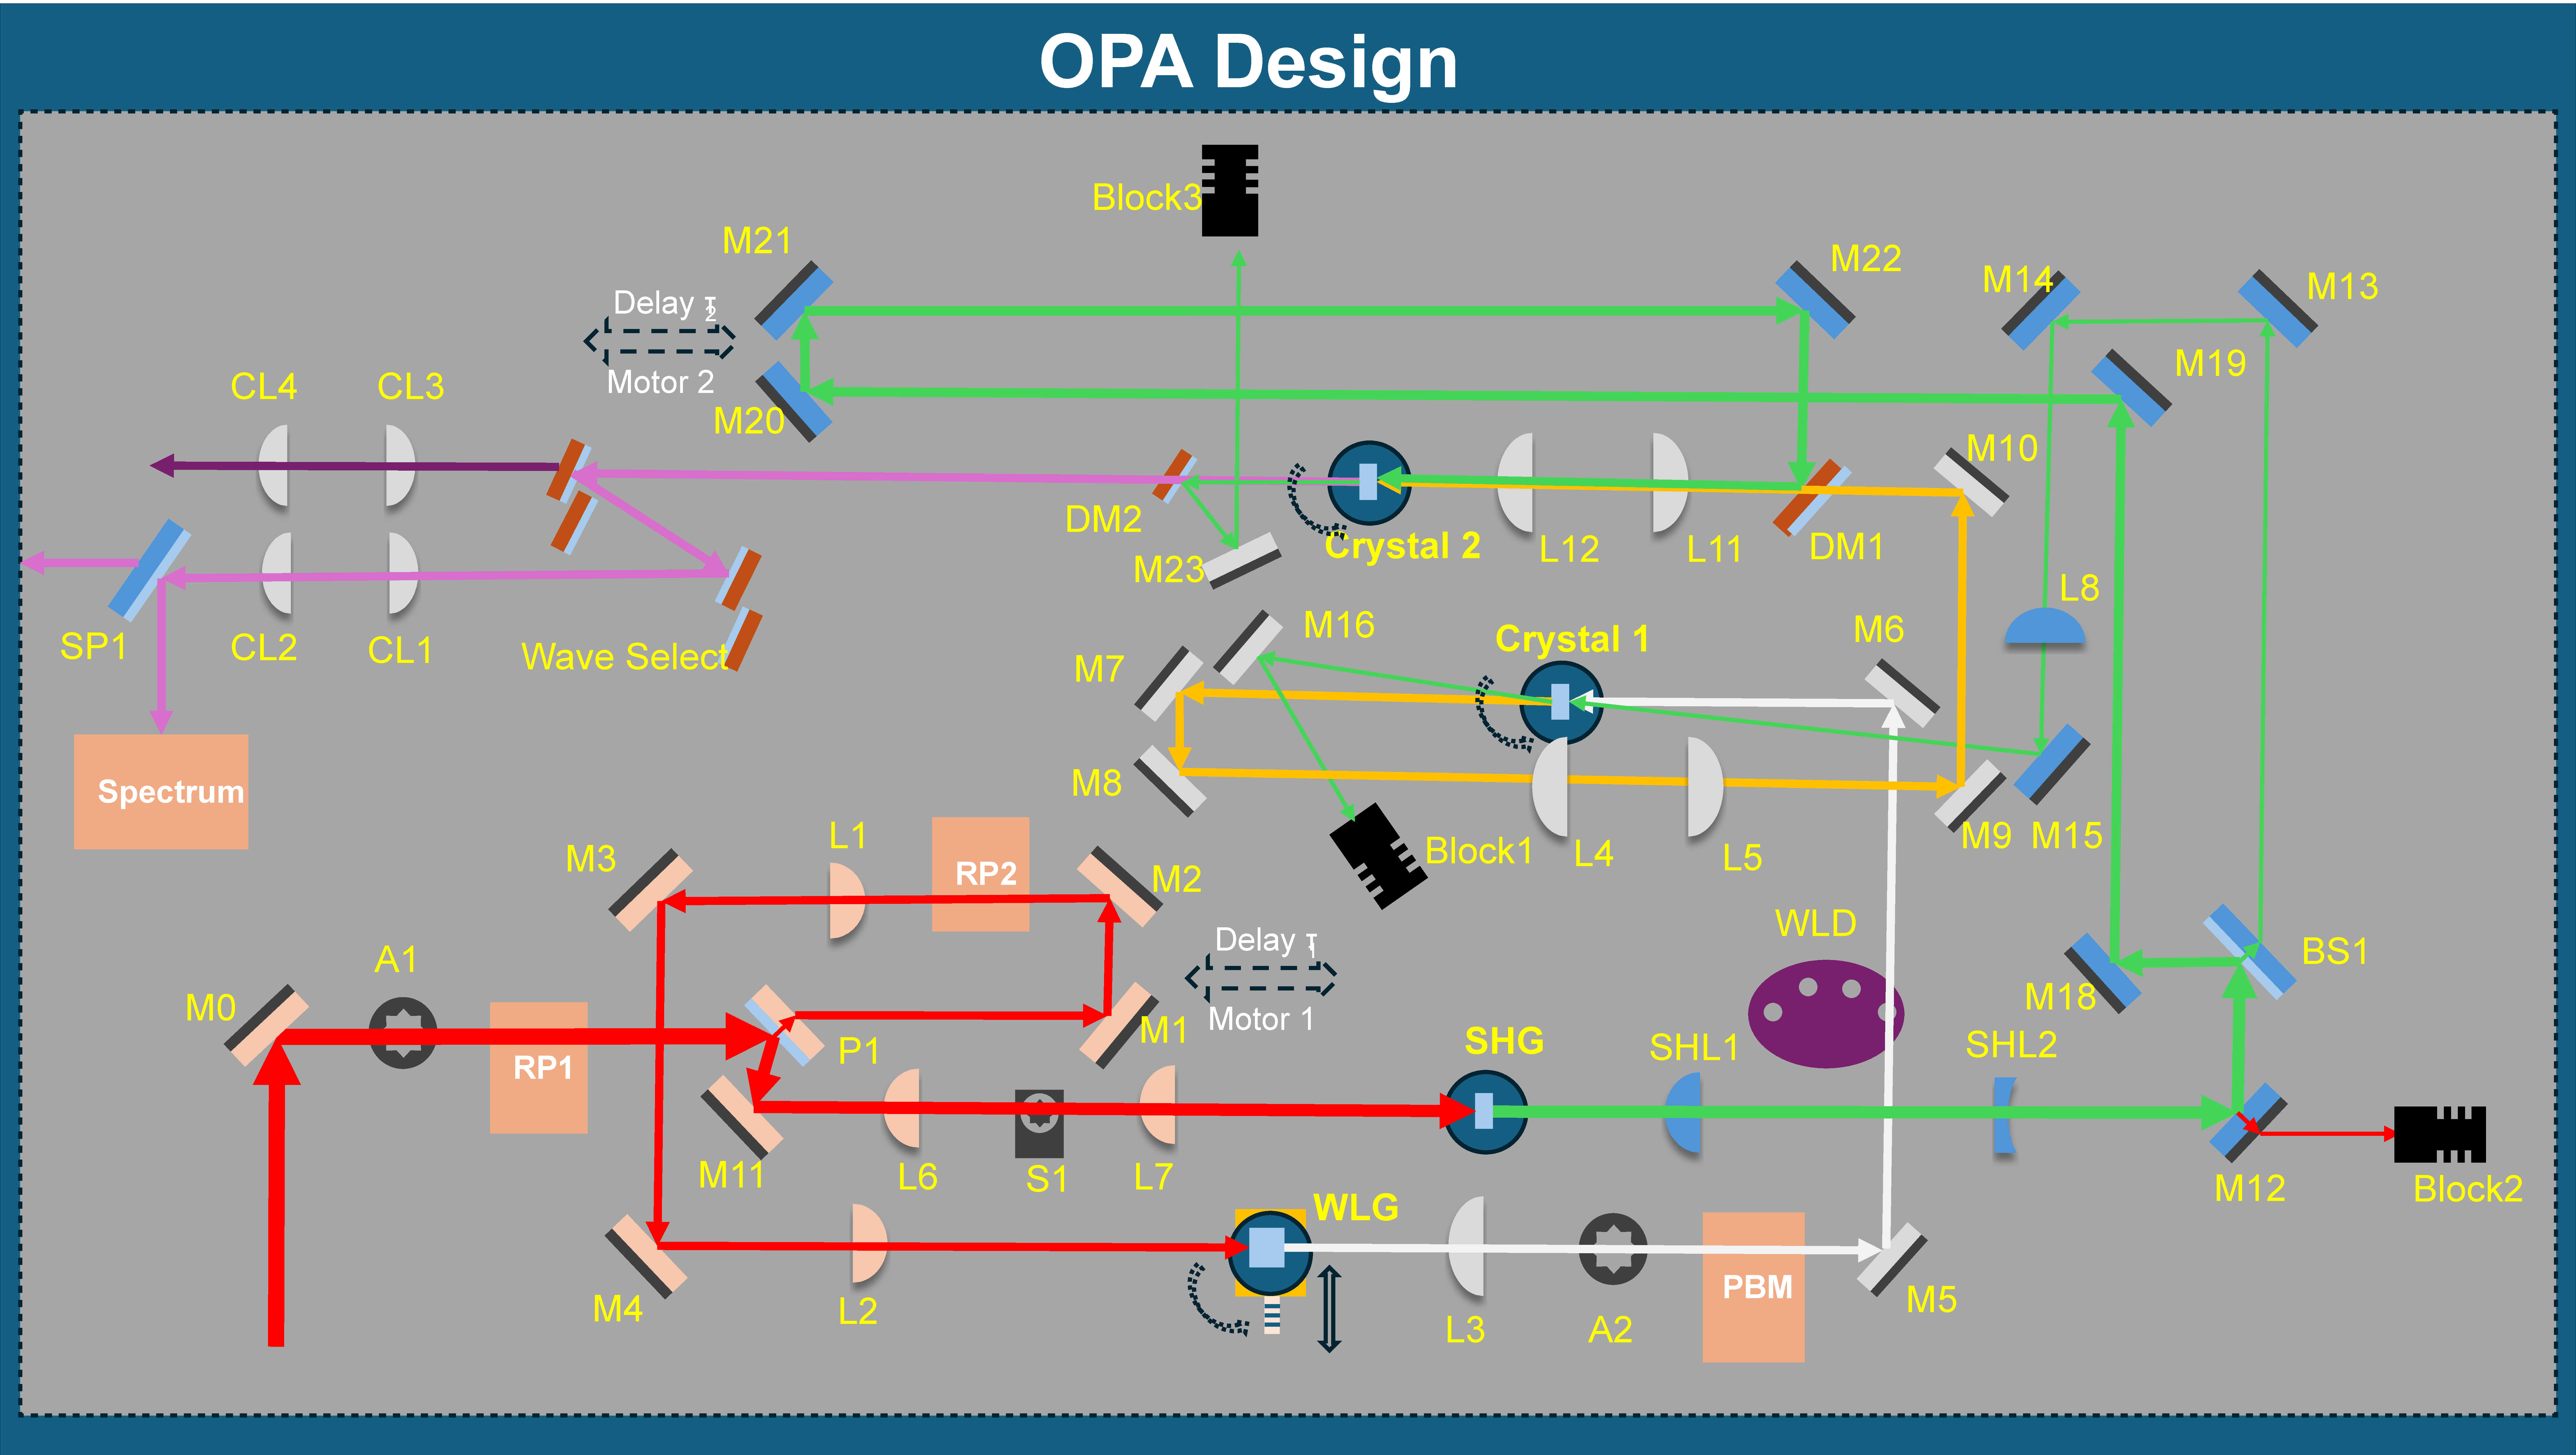
\includegraphics[width=0.7\textwidth]{Fig/FigOPA.pdf}
    \bicaption{OPA 设计光路示意图}{Schematic optical layout of the OPA design}
    \label{fig:OPA_layout}
\end{figure}


在扫描与探测方面，该系统采用 Cambridge 6210H 振镜进行二维扫描，并使用 Hamamatsu H7422P PMT 探测器进行荧光信号采集。系统整体采用固定式架构，具有光路清晰、调试便利和长期稳定性较好的优点；同时其延长臂采用可旋转并可伸长的机械设计，使系统既可用于常规样品台成像，也便于适配活体成像或组织样品成像等实验场景。相较于开放式临时搭建光路，该固定式方案更强调稳定性和可重复性，适合作为多光子成像能力建立与后续模块测试的平台。

通过该系统，本文完成了双光子与三光子联合激发条件下的初步成像实验，获得的代表性成像结果如图~\ref{FigSup01} 所示。实验结果表明，该固定式系统能够实现稳定的多光子成像。在经过棱镜对的脉冲压缩后，最低只需要不到300mW功率即可看清荧光微球样本，在800uW左右能够获得高对比度的结果，验证了激发链路、扫描链路与探测链路设计的可行性。

\begin{figure}[bhtp]
    \centering
    \includegraphics[width=0.85\textwidth]{Fig/FigSup01}
    \bicaption{第一套固定式多光子显微镜系统的代表性成像结果}{Representative imaging results of the first fixed multiphoton microscope system}
    \label{FigSup01}
\end{figure}

% 除基础成像能力验证外，第一套系统还为后续长波激发、多光子色散补偿以及寿命测量链路接入提供了实验基础。尤其是 OPA 通道的引入，使系统具备了从常规双光子成像进一步拓展到长波三光子激发的能力，这对于深层成像和多模态实验具有重要意义。



\section{第二套快速切换多光子显微镜系统设计与搭建}\label{4.3}

在第一套固定式多光子显微镜完成原理验证的基础上，本文进一步面向活体生物成像需求，设计并搭建了第二套快速切换式多光子显微镜系统。与第一套系统相比，该系统不仅支持双光子与三光子激发模式，而且在机械结构、扫描模式和光路切换方式上进行了更深入的工程创新，目标是在保证成像性能的前提下，提高系统的灵活性、可切换性和适配活体实验的能力。

在激发源配置方面，该系统支持双光子与三光子两类激发模式切换：双光子通道由 Spectra-Physics Mai Tai 激光器提供 690--1040\,nm 范围内的飞秒激发；三光子通道则采用 Spectra-Physics Spirit 激光平台提供 1300--1700\,nm 长波激发。通过将两类激发光源集成到同一显微系统中，系统能够根据不同成像深度、样品类型和荧光探针要求，在双光子和三光子工作模式之间进行切换，从而显著提升实验适用范围。

该系统的一个重要创新点在于，其整体机械平台并非采用传统固定式面包板结构，而是构建在定制的 XY 精密位移台之上。位移平台采用骏河精机(SURUGA SEIKI)结构，其中 X 轴行程为 200\,mm，Y 轴行程为 75\,mm，系统定位分辨率可达 2\,$\mu$m。通过将整套显微系统搭载在高精度位移平台上，可在较大范围内对成像区域进行快速定位与切换，尤其适合活体样品或大尺寸组织样品的多区域成像需求。这种``显微系统整体随平台运动''的设计思路不同于常规仅移动样品台的方式，为后续大范围扫描、活体定位与自动化拓展提供了良好基础。

在扫描模块设计方面，本文进一步实现了 galvo/galvo 与 galvo/resonant 两种成像模式的集成，并可根据实验需求在两种模式之间快速切换。其中，galvo/galvo 模式适合高灵活性的常规扫描与 ROI 扫描，而 galvo/resonant 模式则更适用于高速成像场景。为实现共振振镜与普通振镜在同一系统中的兼容，本文专门设计了中继透镜(爱特蒙特光学)结构，用于中继 resonant 振镜与 galvo 振镜之间的空间距离，使两种扫描器件在切换后仍能满足扫描共轭关系和后续中继光路要求。该设计有效解决了不同扫描模块在空间布局与光学共轭上的兼容问题，是本系统实现双扫描模式快速切换的关键。

\begin{figure}[htbp]
    \centering
    \begin{subfigure}{0.52\linewidth}
        \centering
        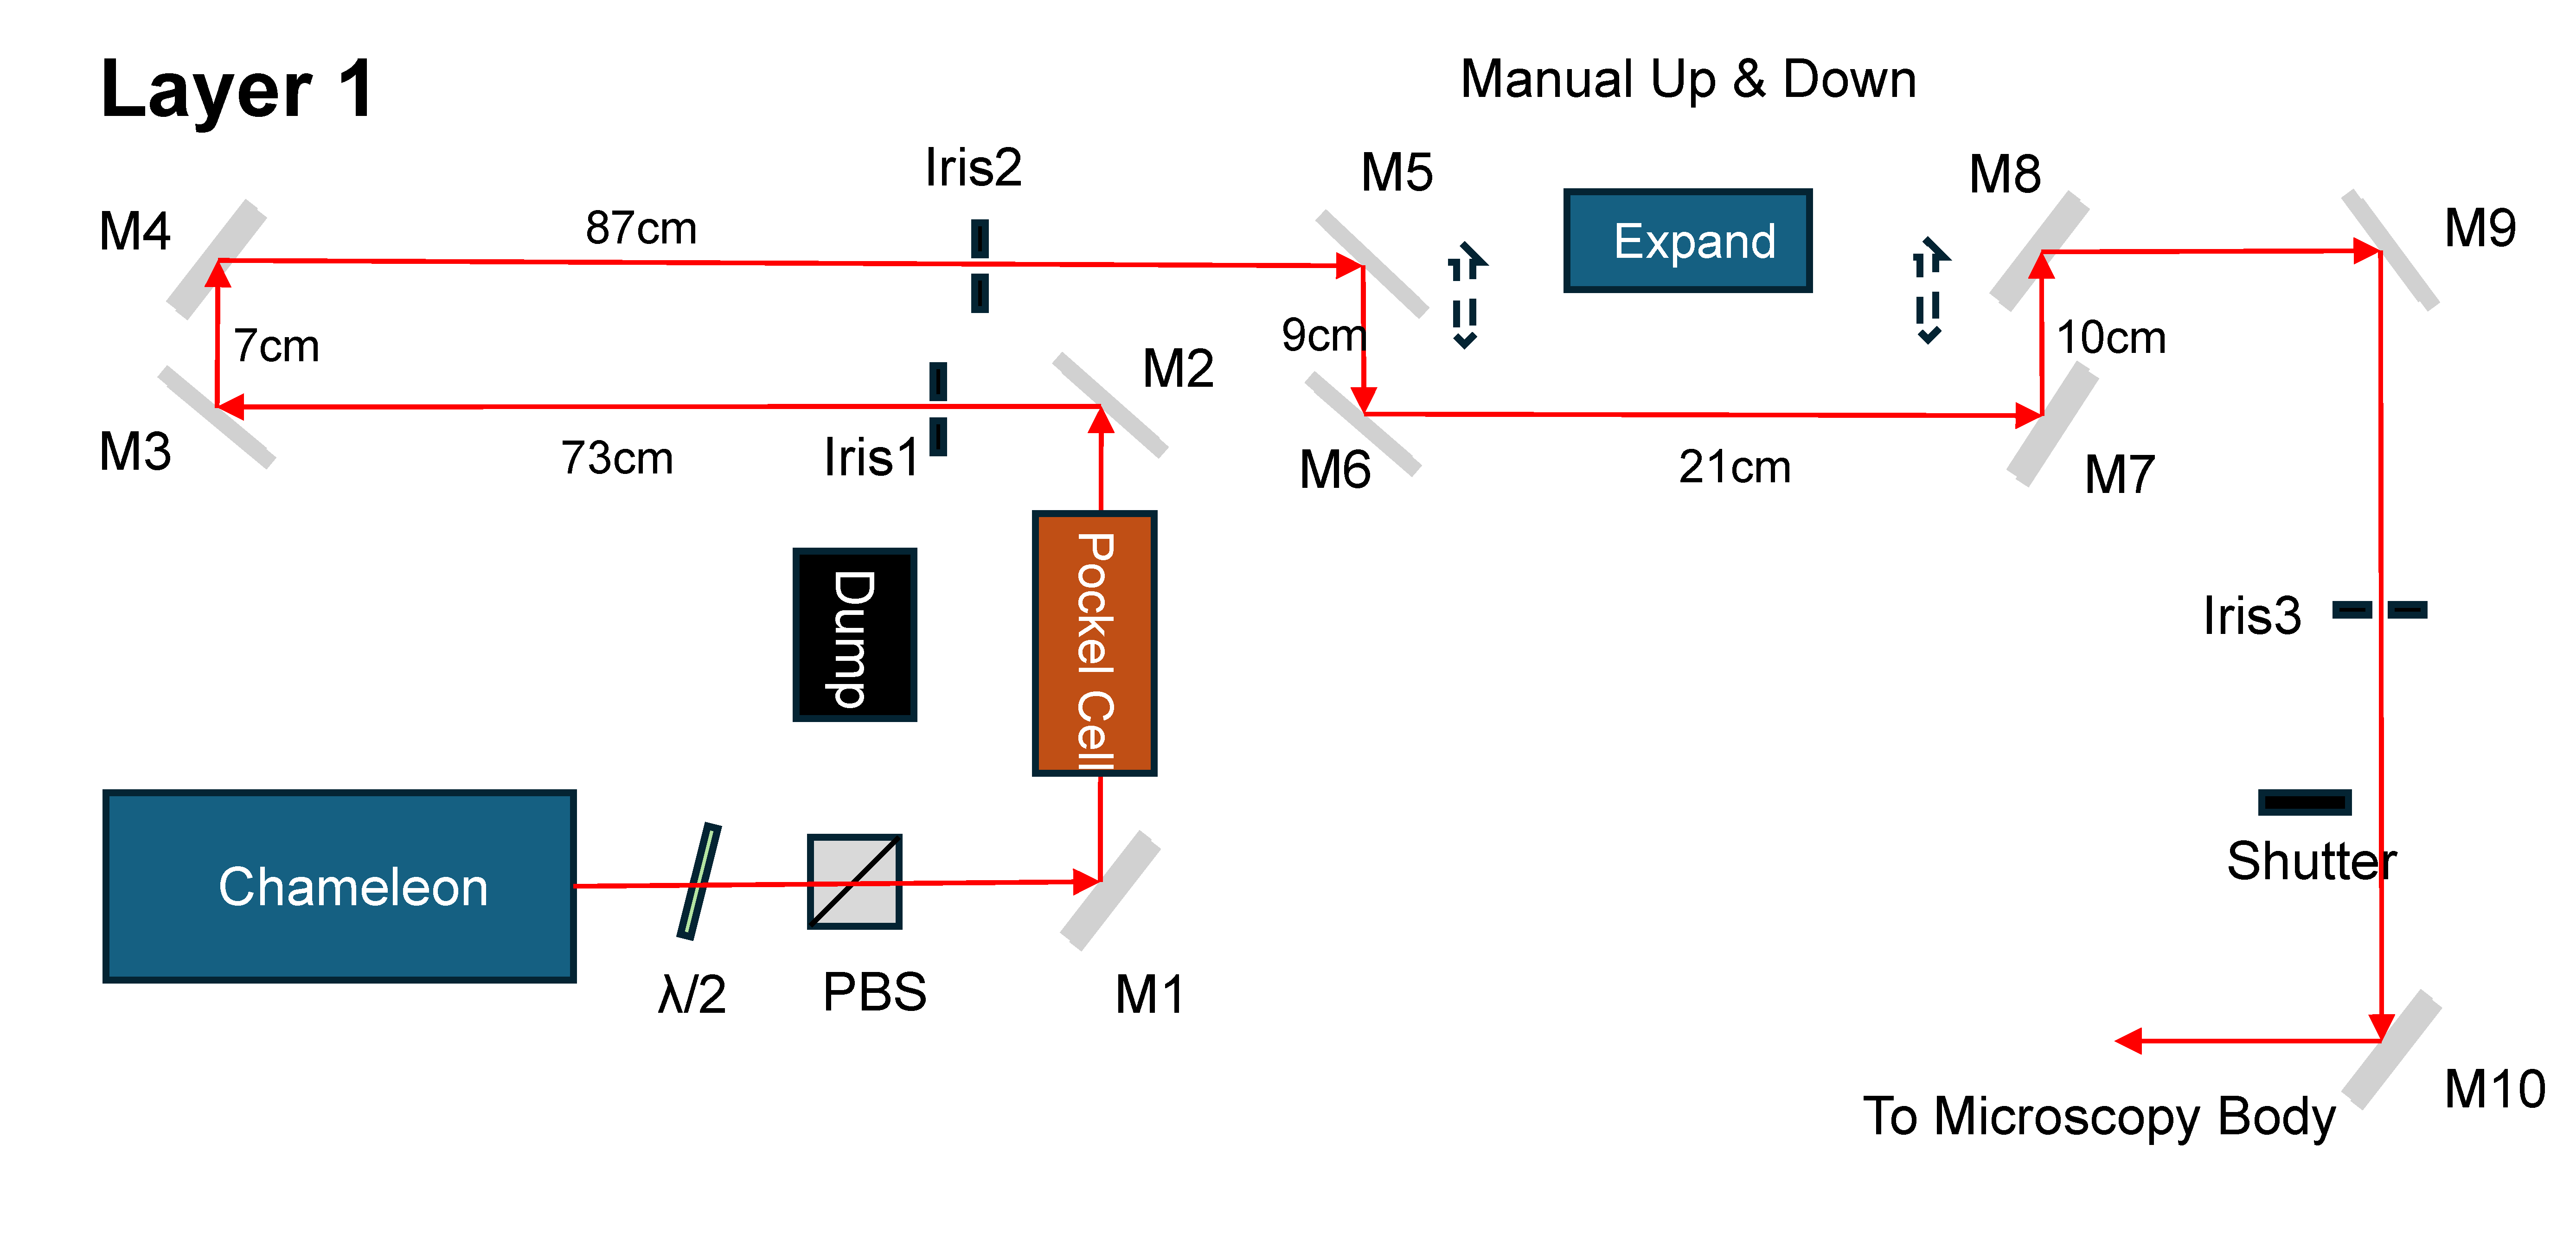
\includegraphics[width=\linewidth]{Fig/Fig3P05.pdf}
        \caption{}
        \label{Fig3P05}
    \end{subfigure}
    \hspace{0.03\linewidth}
    \begin{subfigure}{0.32\linewidth}
        \centering
        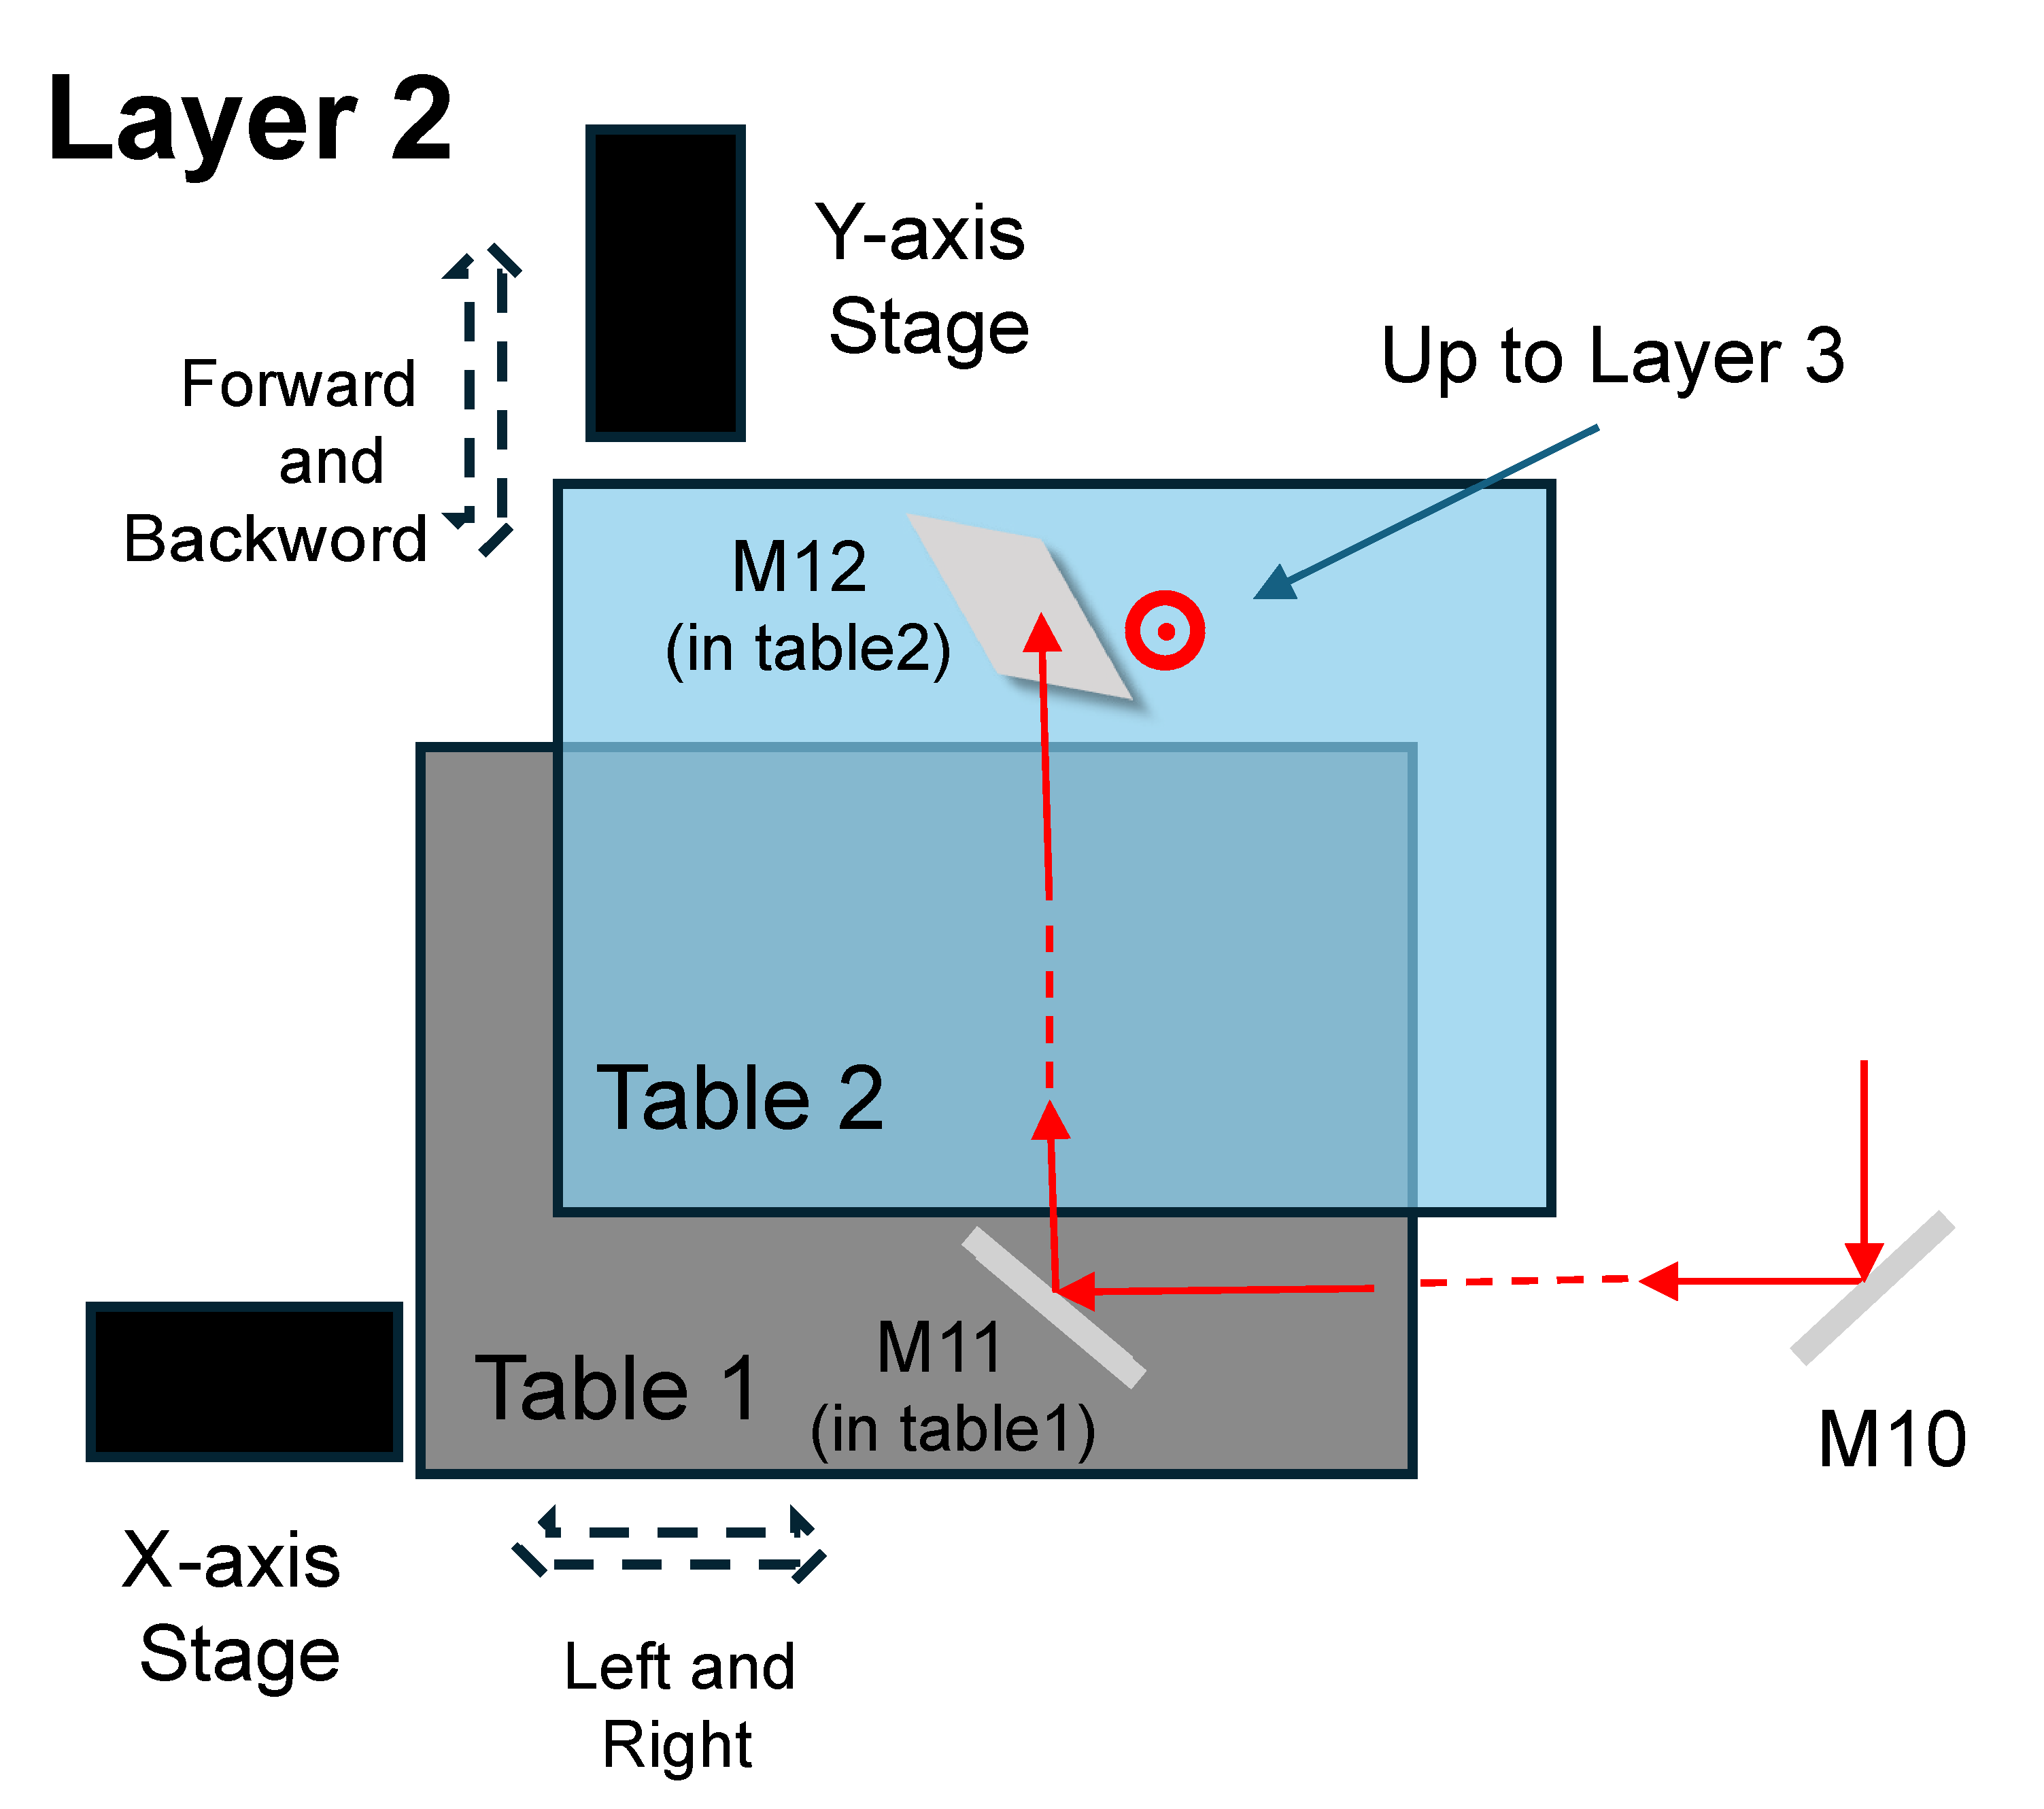
\includegraphics[width=\linewidth]{Fig/Fig3P06.pdf}
        \caption{}
        \label{Fig3P06}
    \end{subfigure}

    \vspace{1em}

    \begin{subfigure}{0.36\linewidth}
        \centering
        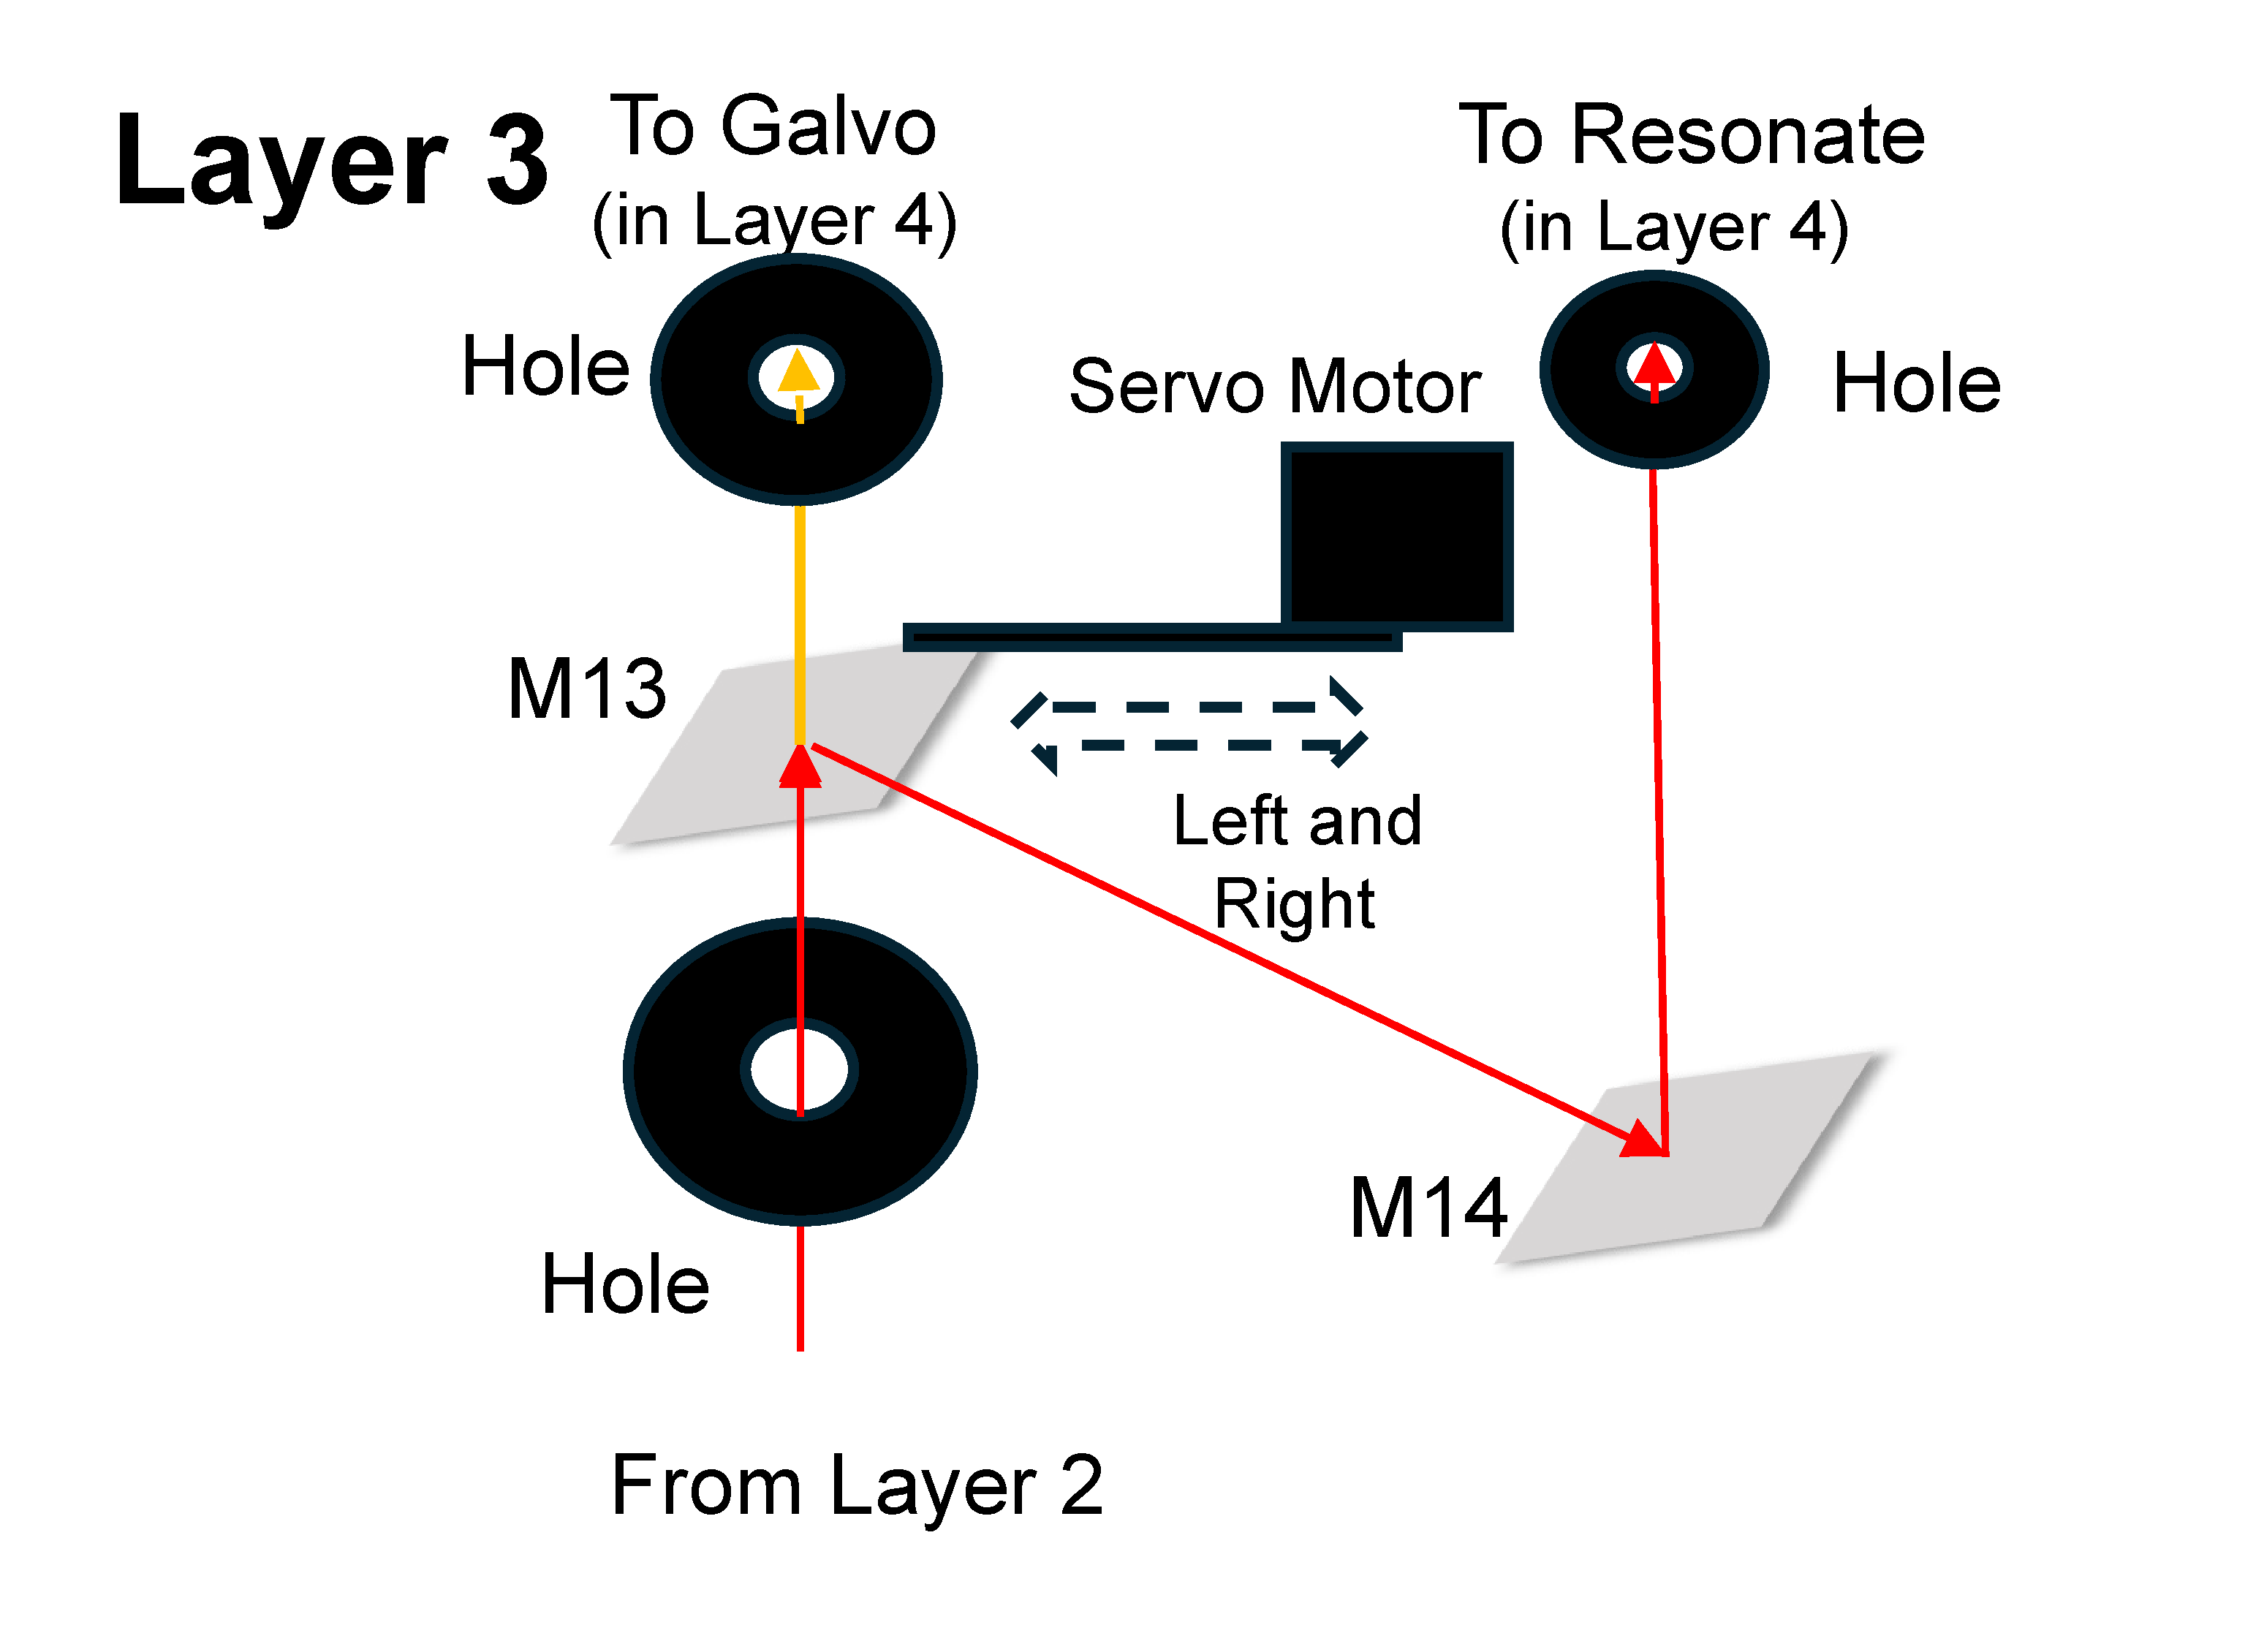
\includegraphics[width=\linewidth]{Fig/Fig3P07.pdf}
        \caption{}
        \label{Fig3P07}
    \end{subfigure}
    \hspace{0.03\linewidth}
    \begin{subfigure}{0.48\linewidth}
        \centering
        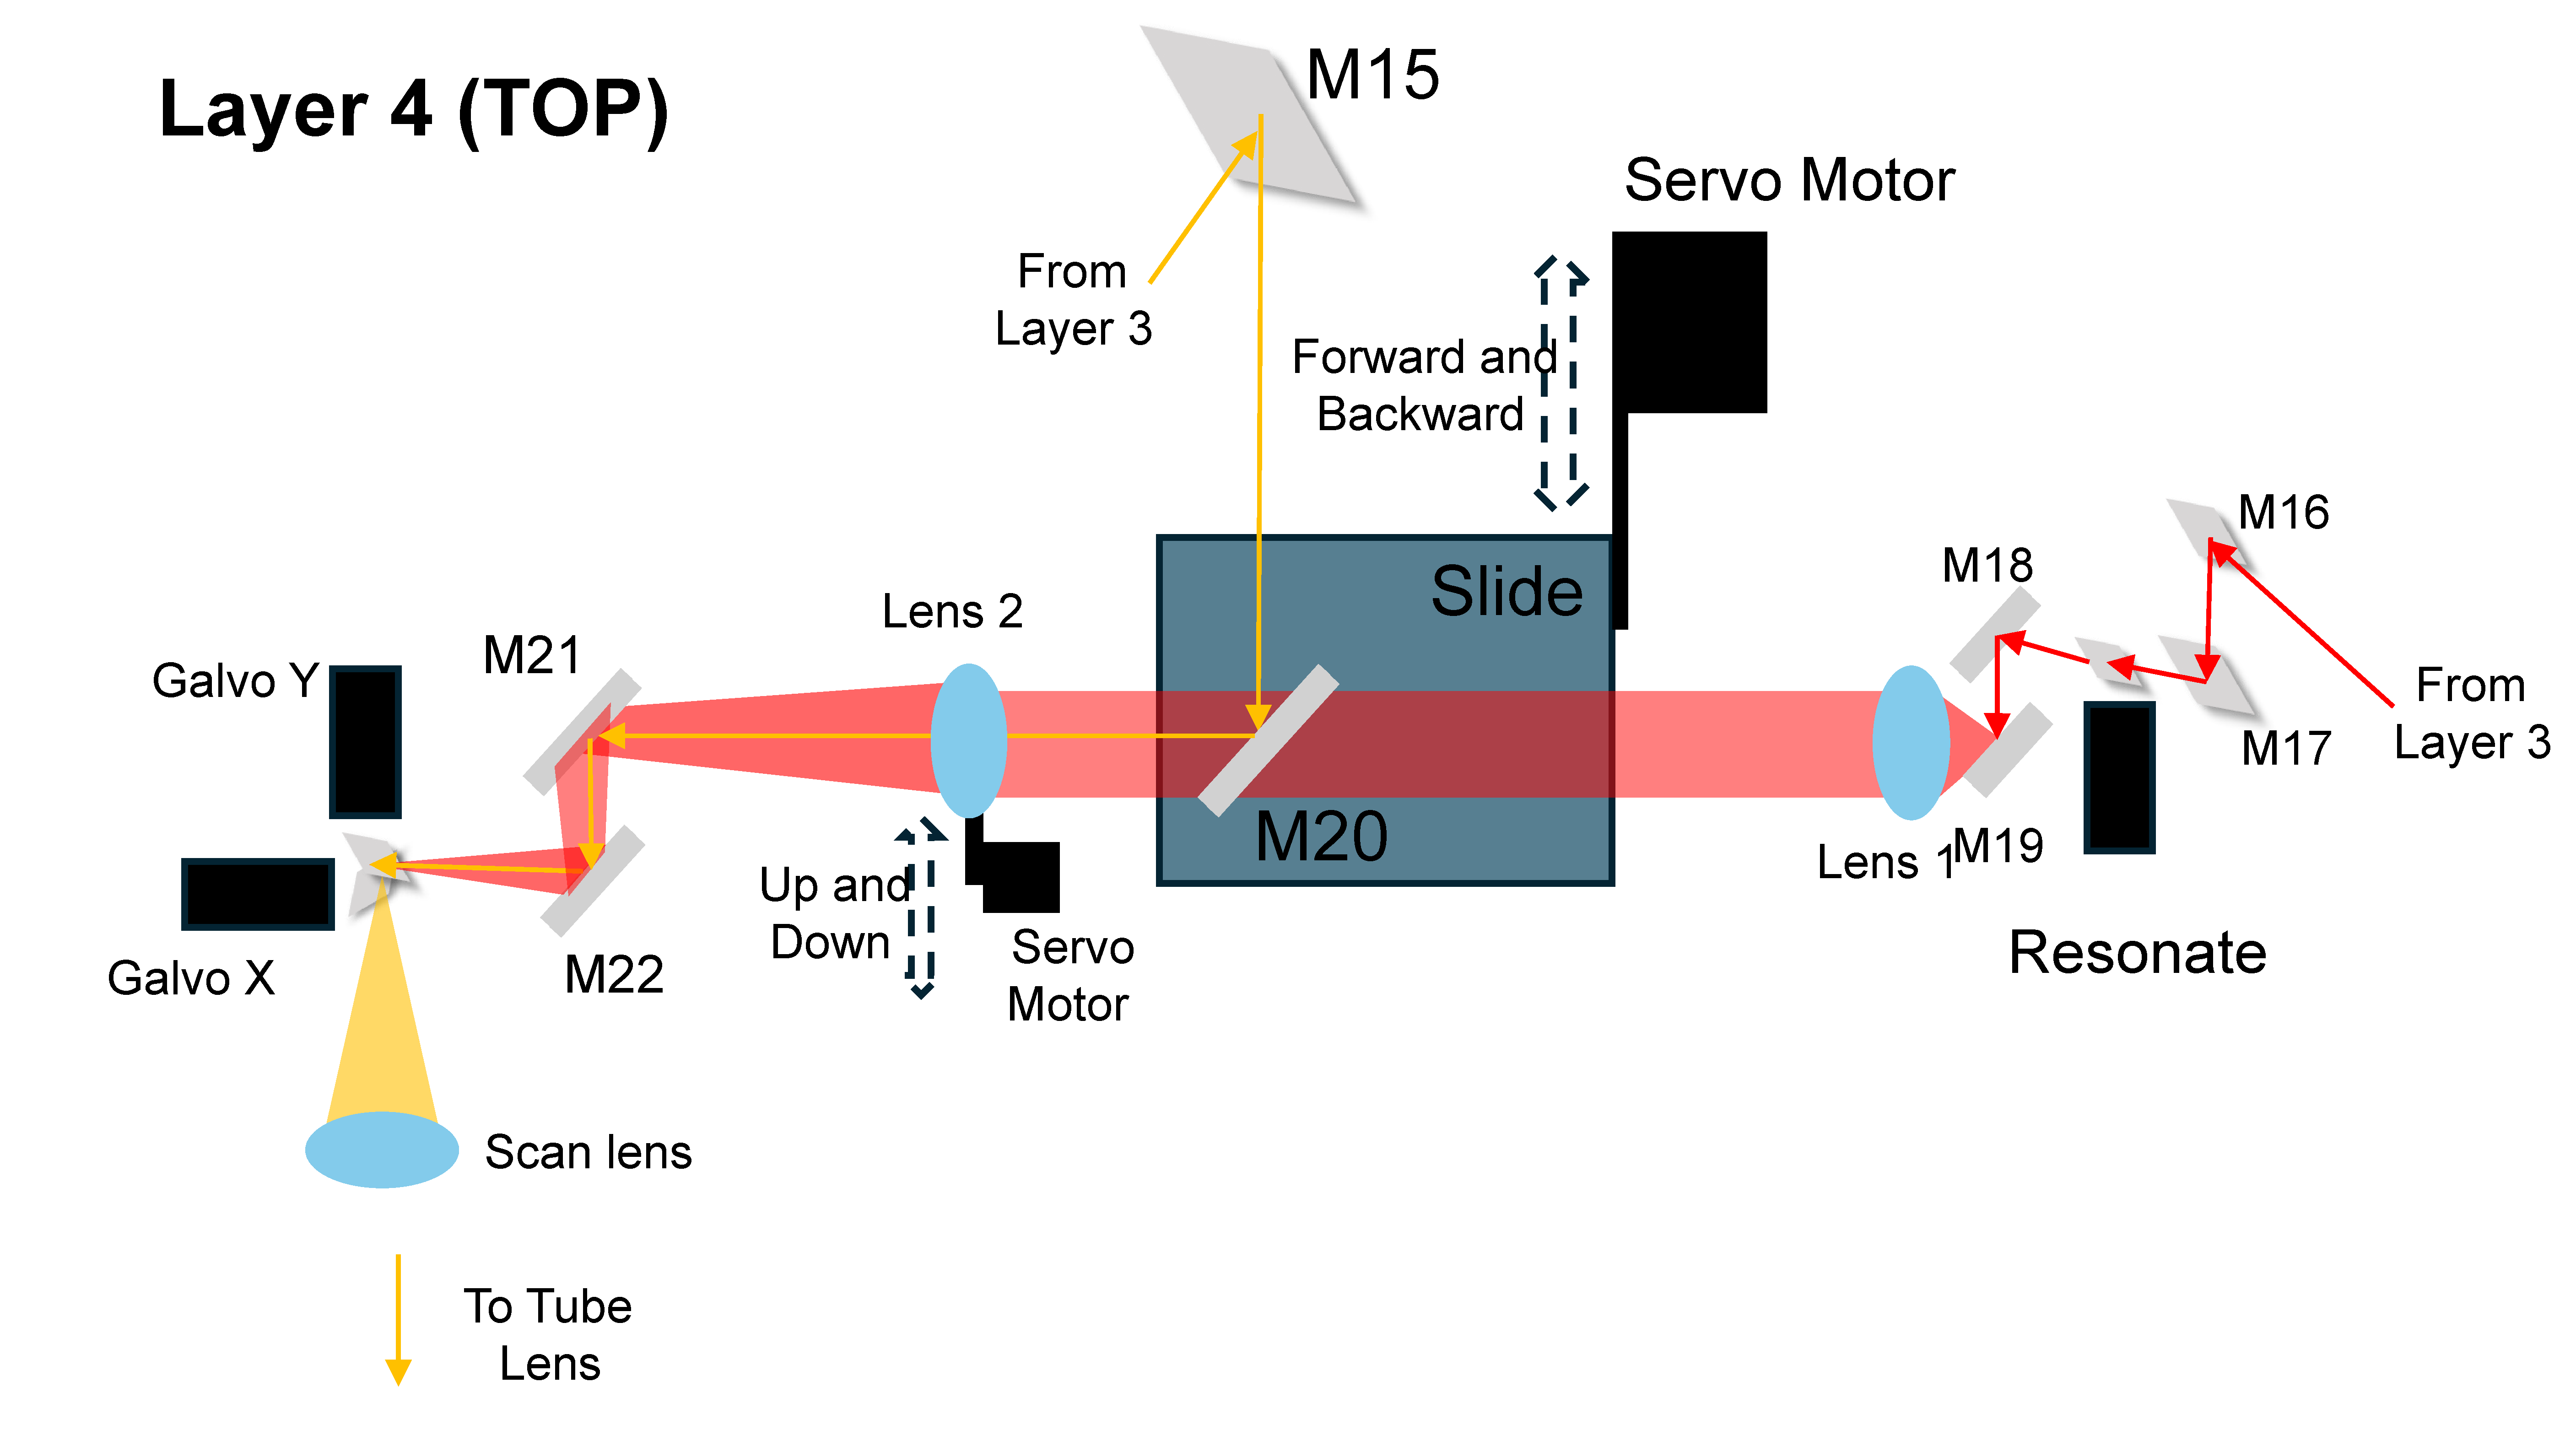
\includegraphics[width=\linewidth]{Fig/Fig3P08.pdf}
        \caption{}
        \label{Fig3P08}
    \end{subfigure}
    \bicaption{第二套快速切换多光子显微镜系统的分层光学布局。(a) 显微镜第二层结构；(b) 显微镜第三层结构；(c) 显微镜第二层实物布局；(d) 显微镜第三层实物布局}{Layered optical layout of the second fast-switching multiphoton microscope system. (a) Second-layer structure; (b) third-layer structure; (c) physical layout of the second layer; (d) physical layout of the third layer}
    \label{Fig3P5-8}
\end{figure}

此外，本文还采用舵机驱动方式实现不同光路之间的自动切换，从而避免了传统手动翻转镜或人工插拔元件带来的重复定位误差和切换效率低的问题。与此同时，系统还设计了可精密移动的 scan lens 对焦结构，通过对扫描透镜位置进行微调，以补偿不同激发模式、不同扫描路径和不同成像深度下的焦点偏移问题。该结构在系统调试和多模式切换过程中表现出较高的灵活性，有助于提高成像焦点位置的一致性和系统重现性。

% 综上，第二套多光子显微镜并非仅是对第一套系统的简单复制，而是在机械平台、扫描结构、光路切换和对焦方式等多个层面进行了系统性创新。其核心特点可概括为：一是双光子/三光子激发兼容；二是 galvo/galvo 与 galvo/resonant 双扫描模式兼容；三是整体搭载于高精度 XY 位移台之上；四是通过舵机切换与 scan lens 精密调焦提高系统切换效率与对准稳定性。这些设计共同构成了该系统面向活体多模态成像需求的重要工程基础。



\section{第二套系统的机械设计与光学优化}\label{4.4}

为验证该快速切换多光子显微镜的工程可行性，本文进一步对系统进行了详细的机械设计与光学布局优化，其结果如图~\ref{Fig3P2-4} 和表~\ref{tab:RelayParam} 所示。图~\ref{Fig3P2-4} 主要展示了系统分层机械布局、顶层扫描结构光学设计示意以及顶层光路的实际尺寸优化结果；表~\ref{tab:RelayParam} 则总结了 galvo/resonant 共用扫描链路中的关键中继元件与主要设计参数。通过图表分离的方式，可以更清晰地呈现系统在有限空间内实现多激发源接入、双扫描模式兼容及多模块切换的整体设计思路。

在机械设计层面，系统采用分层模块化布局，以适应双激发源输入、双扫描模式共存以及多探测模块接入的复杂要求。通过将关键光学元件分布到不同高度层面，系统能够在有限平台空间内保持相对清晰的光路组织，同时为后续增加寿命探测链路、脉冲压缩模块和附加成像模块预留空间。机械结构设计的重点不在于简单固定光学元件，而在于为多模式切换提供重复性高、可维护性强的稳定平台。

在光学设计层面，系统重点优化了不同激发源进入同一主光路时的耦合方式，以及不同扫描模式切换时的共轭关系维持问题。对于 galvo/resonant 模式，由于 resonant 共振镜与 galvo 振镜在空间布局和工作特性上存在差异，若直接拼接，往往会引入中继距离不匹配、瞳面传递失真以及后续扫描像差增大等问题。因此，本文在 resonant 振镜与 galvo 扫描单元之间引入由 75~mm 和 150~mm 胶合透镜组成的中继结构，并结合折叠反射镜对光路进行紧凑化重构，以在有限平台空间内尽可能保持扫描角映射关系和物镜后孔径填充条件的一致性。相关关键元件及设计参数见表~\ref{tab:RelayParam}。该设计是系统实现高速扫描与常规扫描兼容的关键。


\begin{figure}[htbp]
    \centering
    \begin{subfigure}[t]{0.52\linewidth}
        \centering
        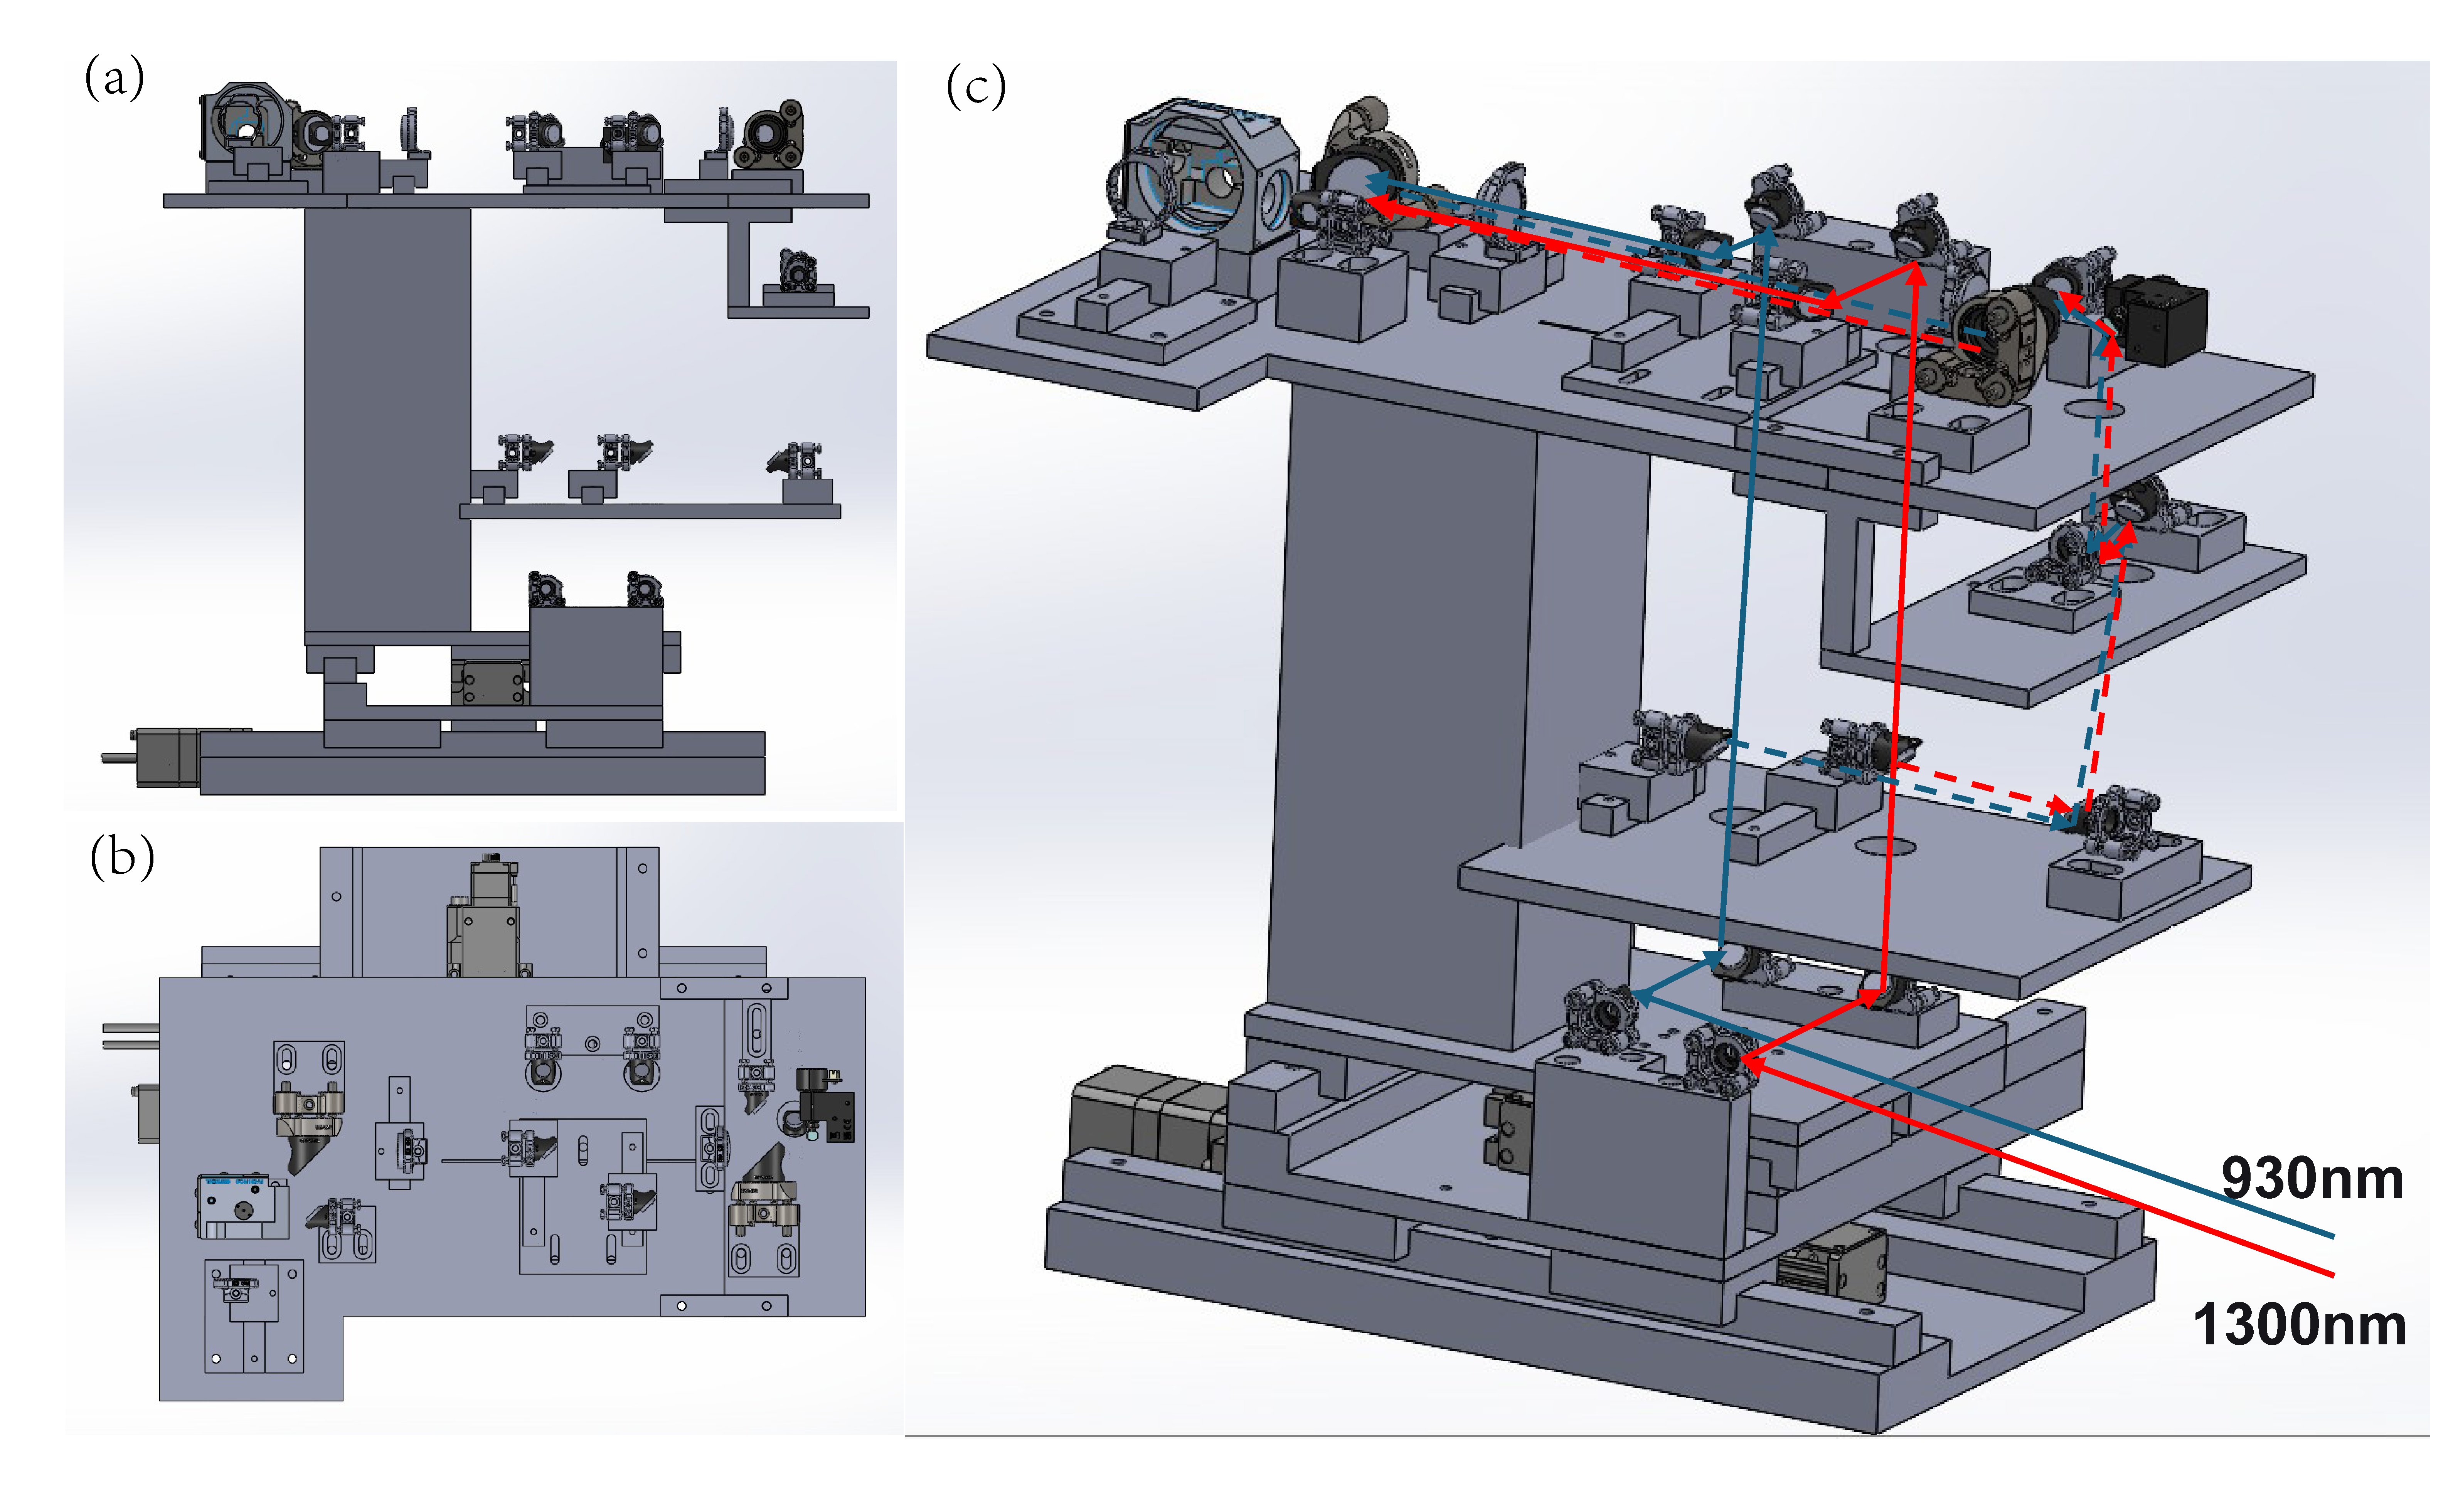
\includegraphics[width=\linewidth]{Fig/Fig3P12.pdf}
        \caption{}
        \label{Fig3P12}
    \end{subfigure}
    \hfill
    \begin{subfigure}[t]{0.39\linewidth}
        \centering
        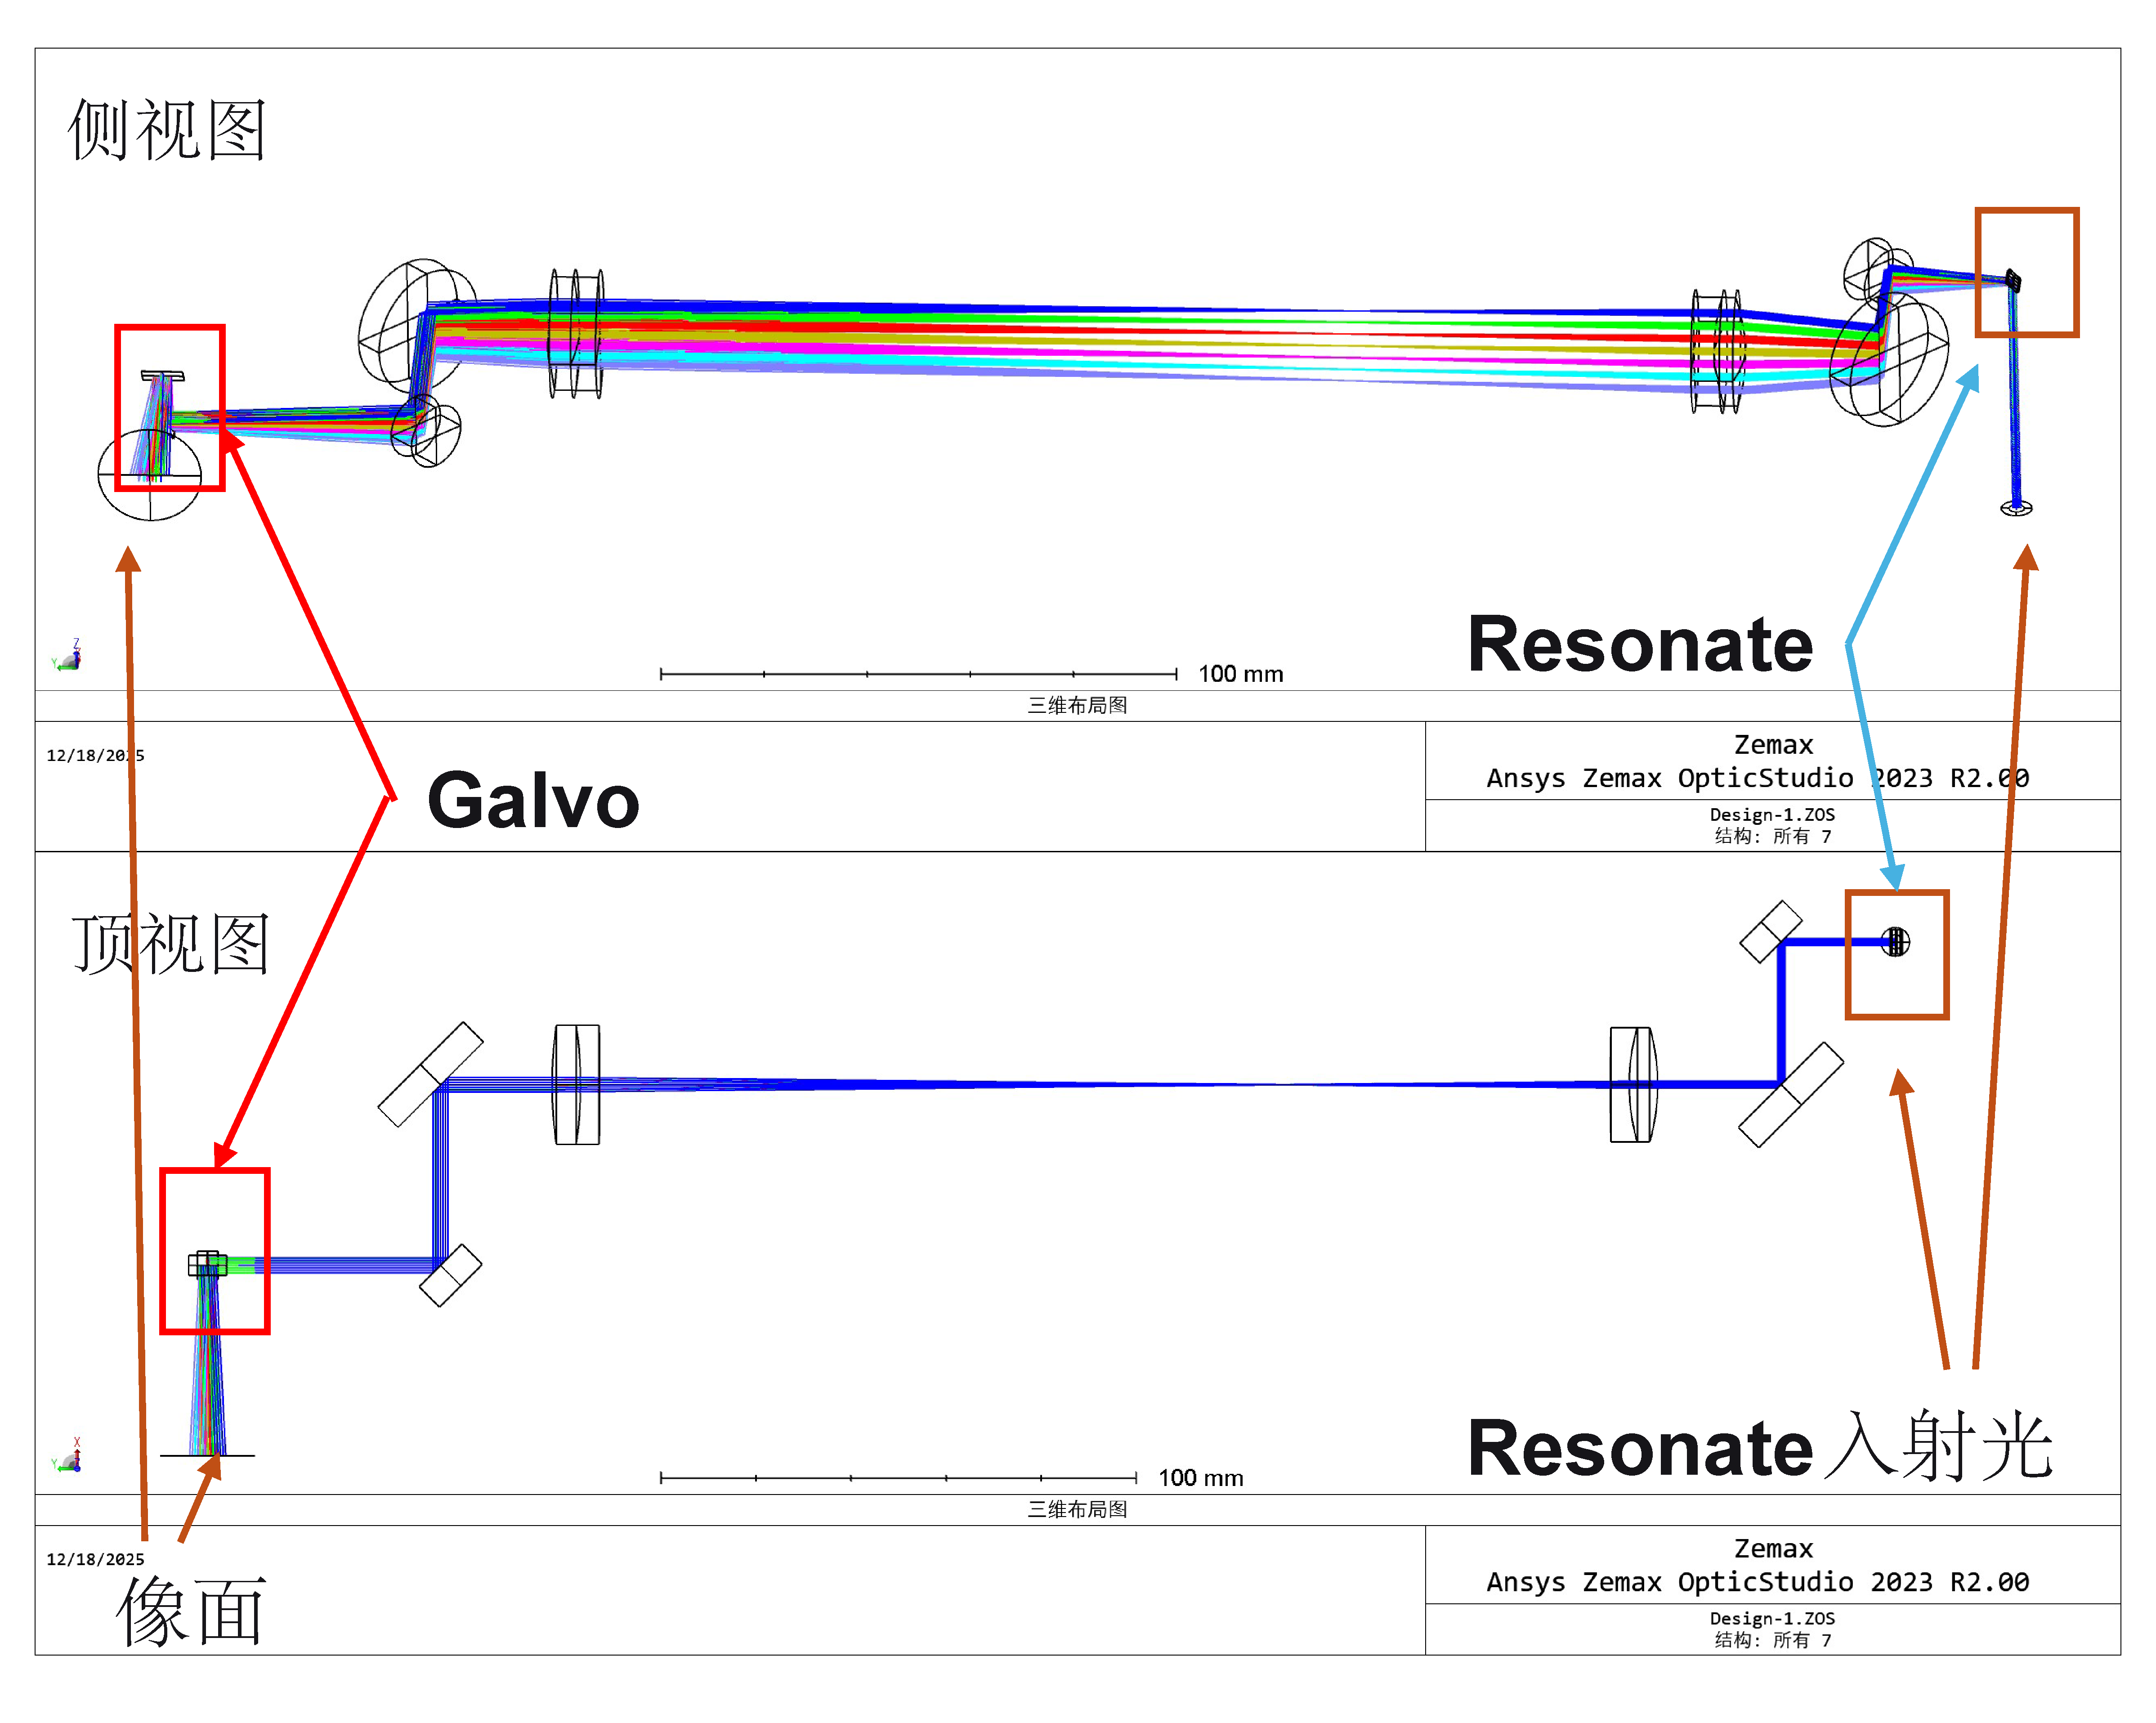
\includegraphics[width=\linewidth]{Fig/Fig3P10.pdf}
        \caption{}
        \label{Fig3P10}
    \end{subfigure}

    \vspace{0.8em}

    \begin{subfigure}[t]{0.78\linewidth}
        \centering
        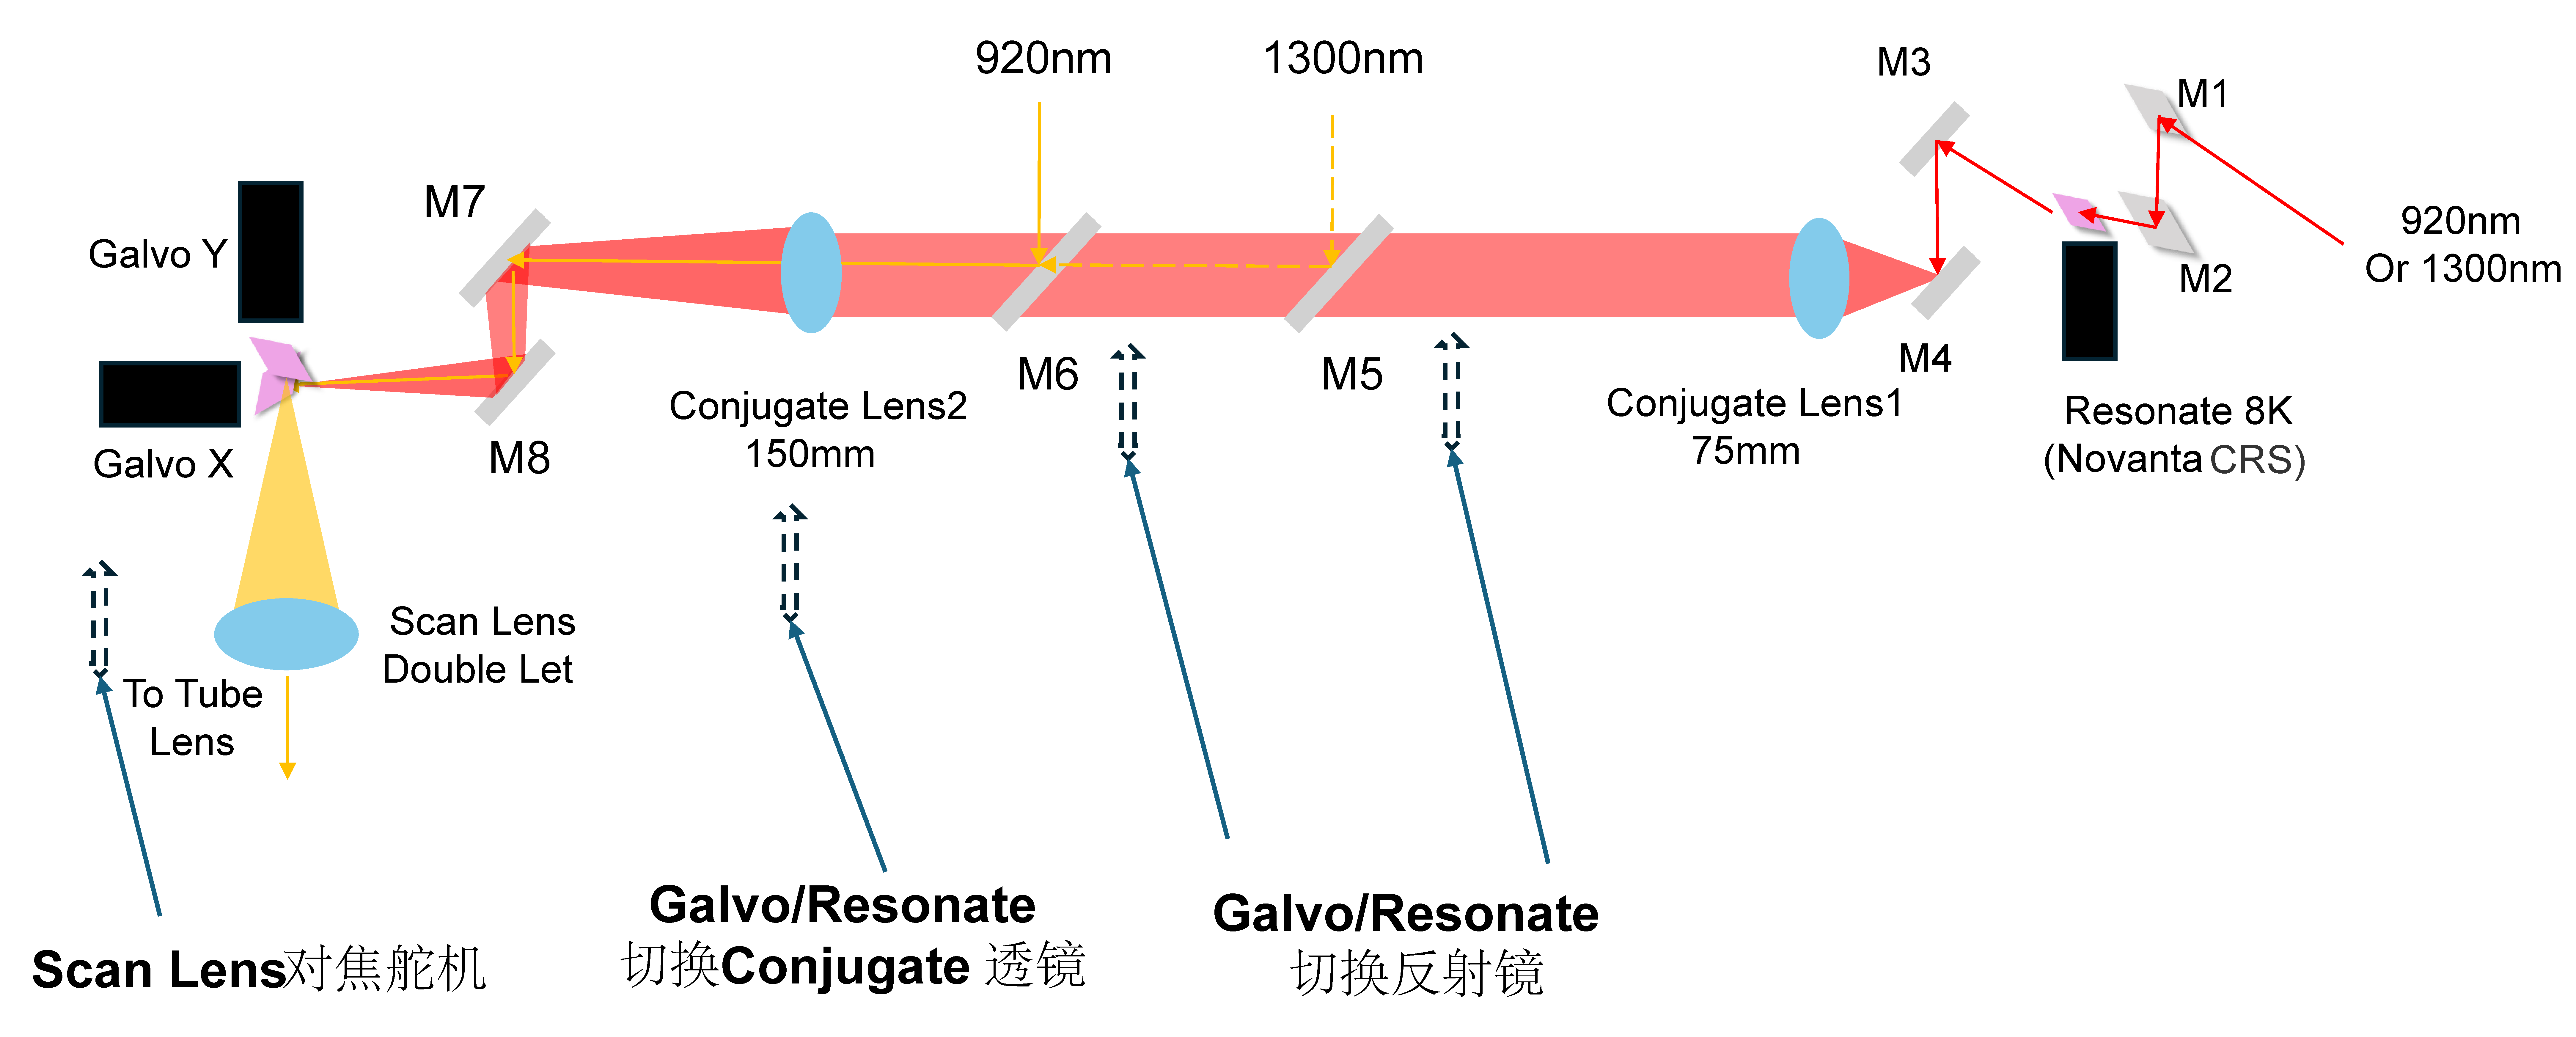
\includegraphics[width=\linewidth]{Fig/Fig3P09.pdf}
        \caption{}
        \label{Fig3P09}
    \end{subfigure}

    \bicaption{第二套快速切换多光子显微镜的机械设计与光学优化。(a) 光学系统机械布局；(b) 顶层扫描结构光学设计示意；(c) 顶层光路设计实际尺寸优化}
    {Mechanical design and optical optimization of the second fast-switching multiphoton microscope. (a) Mechanical layout; (b) optical design schematic of the top scanning structure; (c) optimized top-layer optical path design}
    \label{Fig3P2-4}
\end{figure}


\begin{table}[htbp]
    \centering
    \small
    \setlength{\tabcolsep}{4pt}
    \renewcommand{\arraystretch}{1.15}
    \bicaption{galvo/resonant 共用扫描链路的关键中继元件与设计参数}
    {Key relay components and design parameters of the shared galvo/resonant scanning path}
    \label{tab:RelayParam}
    \begin{tabularx}{\textwidth}{p{2.5cm} p{3.4cm} X p{1.8cm}}
        \hline
        元件/模块 & 关键参数 & 主要作用 & 备注 \\
        \hline
        Resonant 振镜 & 高速扫描输入；至后续中继段间隔约 24~mm & 提供 resonant 模式下的高速扫描入口 & 共振扫描模式 \\
        \hline
        第一、第二反射镜 & 两级折叠反射 & 改变传播方向并压缩横向占用空间 & 便于紧凑布局 \\
        \hline
        75~mm 胶合透镜组 & 焦距 75~mm；玻璃材料为 N-LAK22 / N-SF6 & 实现第一段瞳面中继与扫描角映射 & 中继前组 \\
        \hline
        150~mm 胶合透镜组 & 焦距 150~mm；玻璃材料为 N-SF6 / N-LAK22 & 与 75~mm 透镜组共同构成中继望远结构 & 中继后组 \\
        \hline
        第三、第四反射镜 & 折叠段距离38~mm和49~mm & 压缩光路并完成方向校正 & 适配平台空间 \\
        \hline
        X-Galvo / Y-Galvo & 双轴正交扫描；相关间隔10~mm和40~mm & 实现常规双轴扫描与后续主光路共轭 & galvo 模式核心 \\
        \hline
    \end{tabularx}
\end{table}


同时，SL精密移动对焦结构的引入，使系统在不同激发光路和不同扫描模式下均可通过微调方式修正焦面位置偏移。与传统通过样品台或物镜整体粗调对焦不同，该方案更适合用于多模式快速切换时的小范围精密补偿，在保证系统整体稳定性的同时提升了调试效率。

最终完成的第二套多光子显微镜系统实物如图~\ref{figReal2-3} 所示。实验结果表明，该系统能够在有限空间内实现多激发源接入、双扫描模式切换以及高精度样品定位，为后续活体成像和多光子荧光寿命成像实验提供了稳定的平台基础。

\begin{figure}[htbp]
    \centering
    \begin{subfigure}[b]{0.45\textwidth}
        \centering
        \includegraphics[width=\textwidth]{Fig/FigReal02.pdf}
        \caption{}
        \label{figReal02}
    \end{subfigure}
    \vspace{0.3cm}
    \begin{subfigure}[b]{0.45\textwidth}
        \centering
        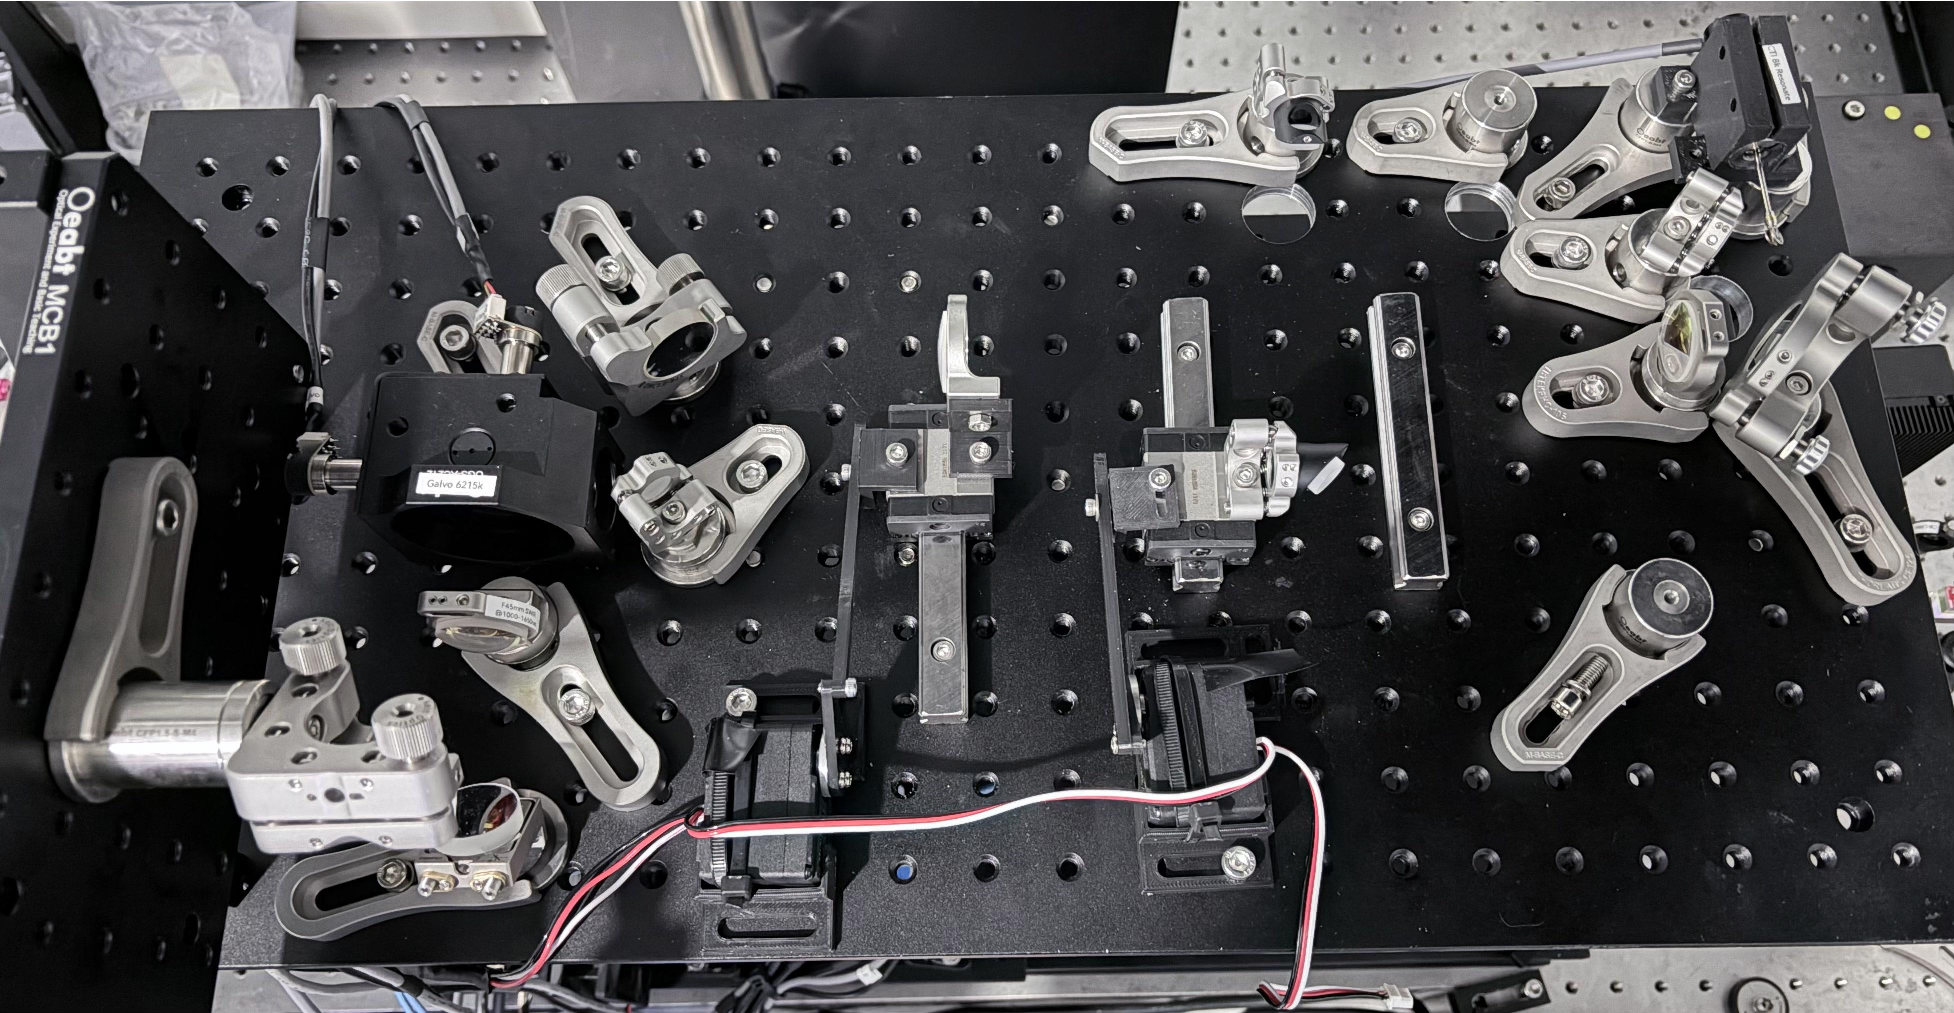
\includegraphics[width=\textwidth]{Fig/FigReal03.pdf}
        \caption{}
        \label{figReal03}
    \end{subfigure}
    \bicaption{第二套快速切换多光子显微镜系统的实物搭建结果。(a) 多光子系统整体；(b) 多光子系统顶层光路}{Photographs of the assembled second fast-switching multiphoton microscope system. (a) Multi photon system as a whole; (b) Top layer optical path of multiphoton system}
    \label{figReal2-3}
\end{figure}




% 除系统实物搭建外，本文还对该平台的成像能力进行了初步验证。相关实验结果表明，系统在双光子激发条件下能够稳定获得样品图像，并具备进一步扩展至三光子成像和荧光寿命成像的条件。与第一套固定式系统相比，第二套系统虽然结构更加复杂，但在切换效率、定位能力和活体成像适配性方面具有明显优势，因而更适合作为后续多模态活体成像实验的平台。

% 总体而言，本文完成了两套多光子显微镜系统的设计与搭建：第一套系统侧重于双光子/三光子联合激发能力建立与长波激发链路验证；第二套系统则在此基础上进一步实现了机械平台、扫描模式、光路切换和精密对焦等多方面创新。两套系统分别对应``能力建立''和``平台优化''两个目标，共同构成了本文多光子荧光寿命显微系统研究的实验基础。




\section{多光子系统中的脉冲压缩与脉宽表征}\label{4.5}

在多光子显微成像系统中，荧光信号的产生依赖于焦点处极高的瞬时峰值功率。对于双光子和三光子激发过程，荧光信号分别近似与光强的二次方和三次方成正比，因此在平均功率一定时，脉冲越短、峰值功率越高，多光子激发效率越高。对于重复频率为 $f$、脉冲宽度为 $\tau$ 的超短脉冲激光，其峰值功率近似与 $1/(f\tau)$ 成正比。因此，当飞秒脉冲在显微系统中传播并发生展宽时，焦点处峰值功率会明显下降，从而直接削弱多光子激发效率，导致成像亮度下降、信噪比降低，并限制系统的有效成像深度。

需要强调的是，这里随脉冲宽度和重复频率变化的是多光子激发效率和最终信号强度，而不是样品本身的荧光量子产率。荧光量子产率是由荧光分子的内禀性质决定的，而脉冲压缩的作用在于减小脉冲宽度、恢复样品处的高峰值功率，从而提升多光子激发概率，改善成像信号质量。因此，在多光子显微镜中进行脉冲压缩，本质上是为了在平均功率受限的条件下提高焦点处瞬时光强，增强多光子激发信号，并降低因盲目提高平均功率而带来的光漂白、光毒性和热损伤风险。

在实际多光子显微镜中，激光脉冲在传播过程中会依次经过扫描镜、扫描透镜、管透镜、分光镜、窗口片、物镜以及样品上方的其他光学介质。这些元件通常都会引入正的群延迟色散(Group Delay Dispersion, GDD)，使飞秒脉冲在到达样品前发生显著展宽。尤其是在高数值孔径物镜和较长光路条件下，系统总色散往往不可忽略。因此，为了使脉冲在样品焦点处尽可能恢复到接近傅里叶变换极限的脉宽，需要在激光进入显微系统之前预先引入负色散补偿装置，以抵消整个成像链路累积的正色散。



\subsection{脉冲压缩器设计与色散补偿方案分析}\label{4.5.1}

在超短脉冲色散管理中，除棱镜对和啁啾镜等方案外，基于衍射光栅的展宽/压缩结构也是最常用的技术路线之一。光栅结构通常能够提供较大的色散调节范围，因此在需要较强群延迟色散补偿的系统中具有重要应用价值。根据成像与折返光路设计方式的不同，典型的光栅展宽器可进一步分为 Treacy 型、Martinez 型和 Öffner 型等结构。

\begin{figure}[htbp]
    \centering
    \begin{subfigure}[b]{0.25\textwidth}
        \centering
        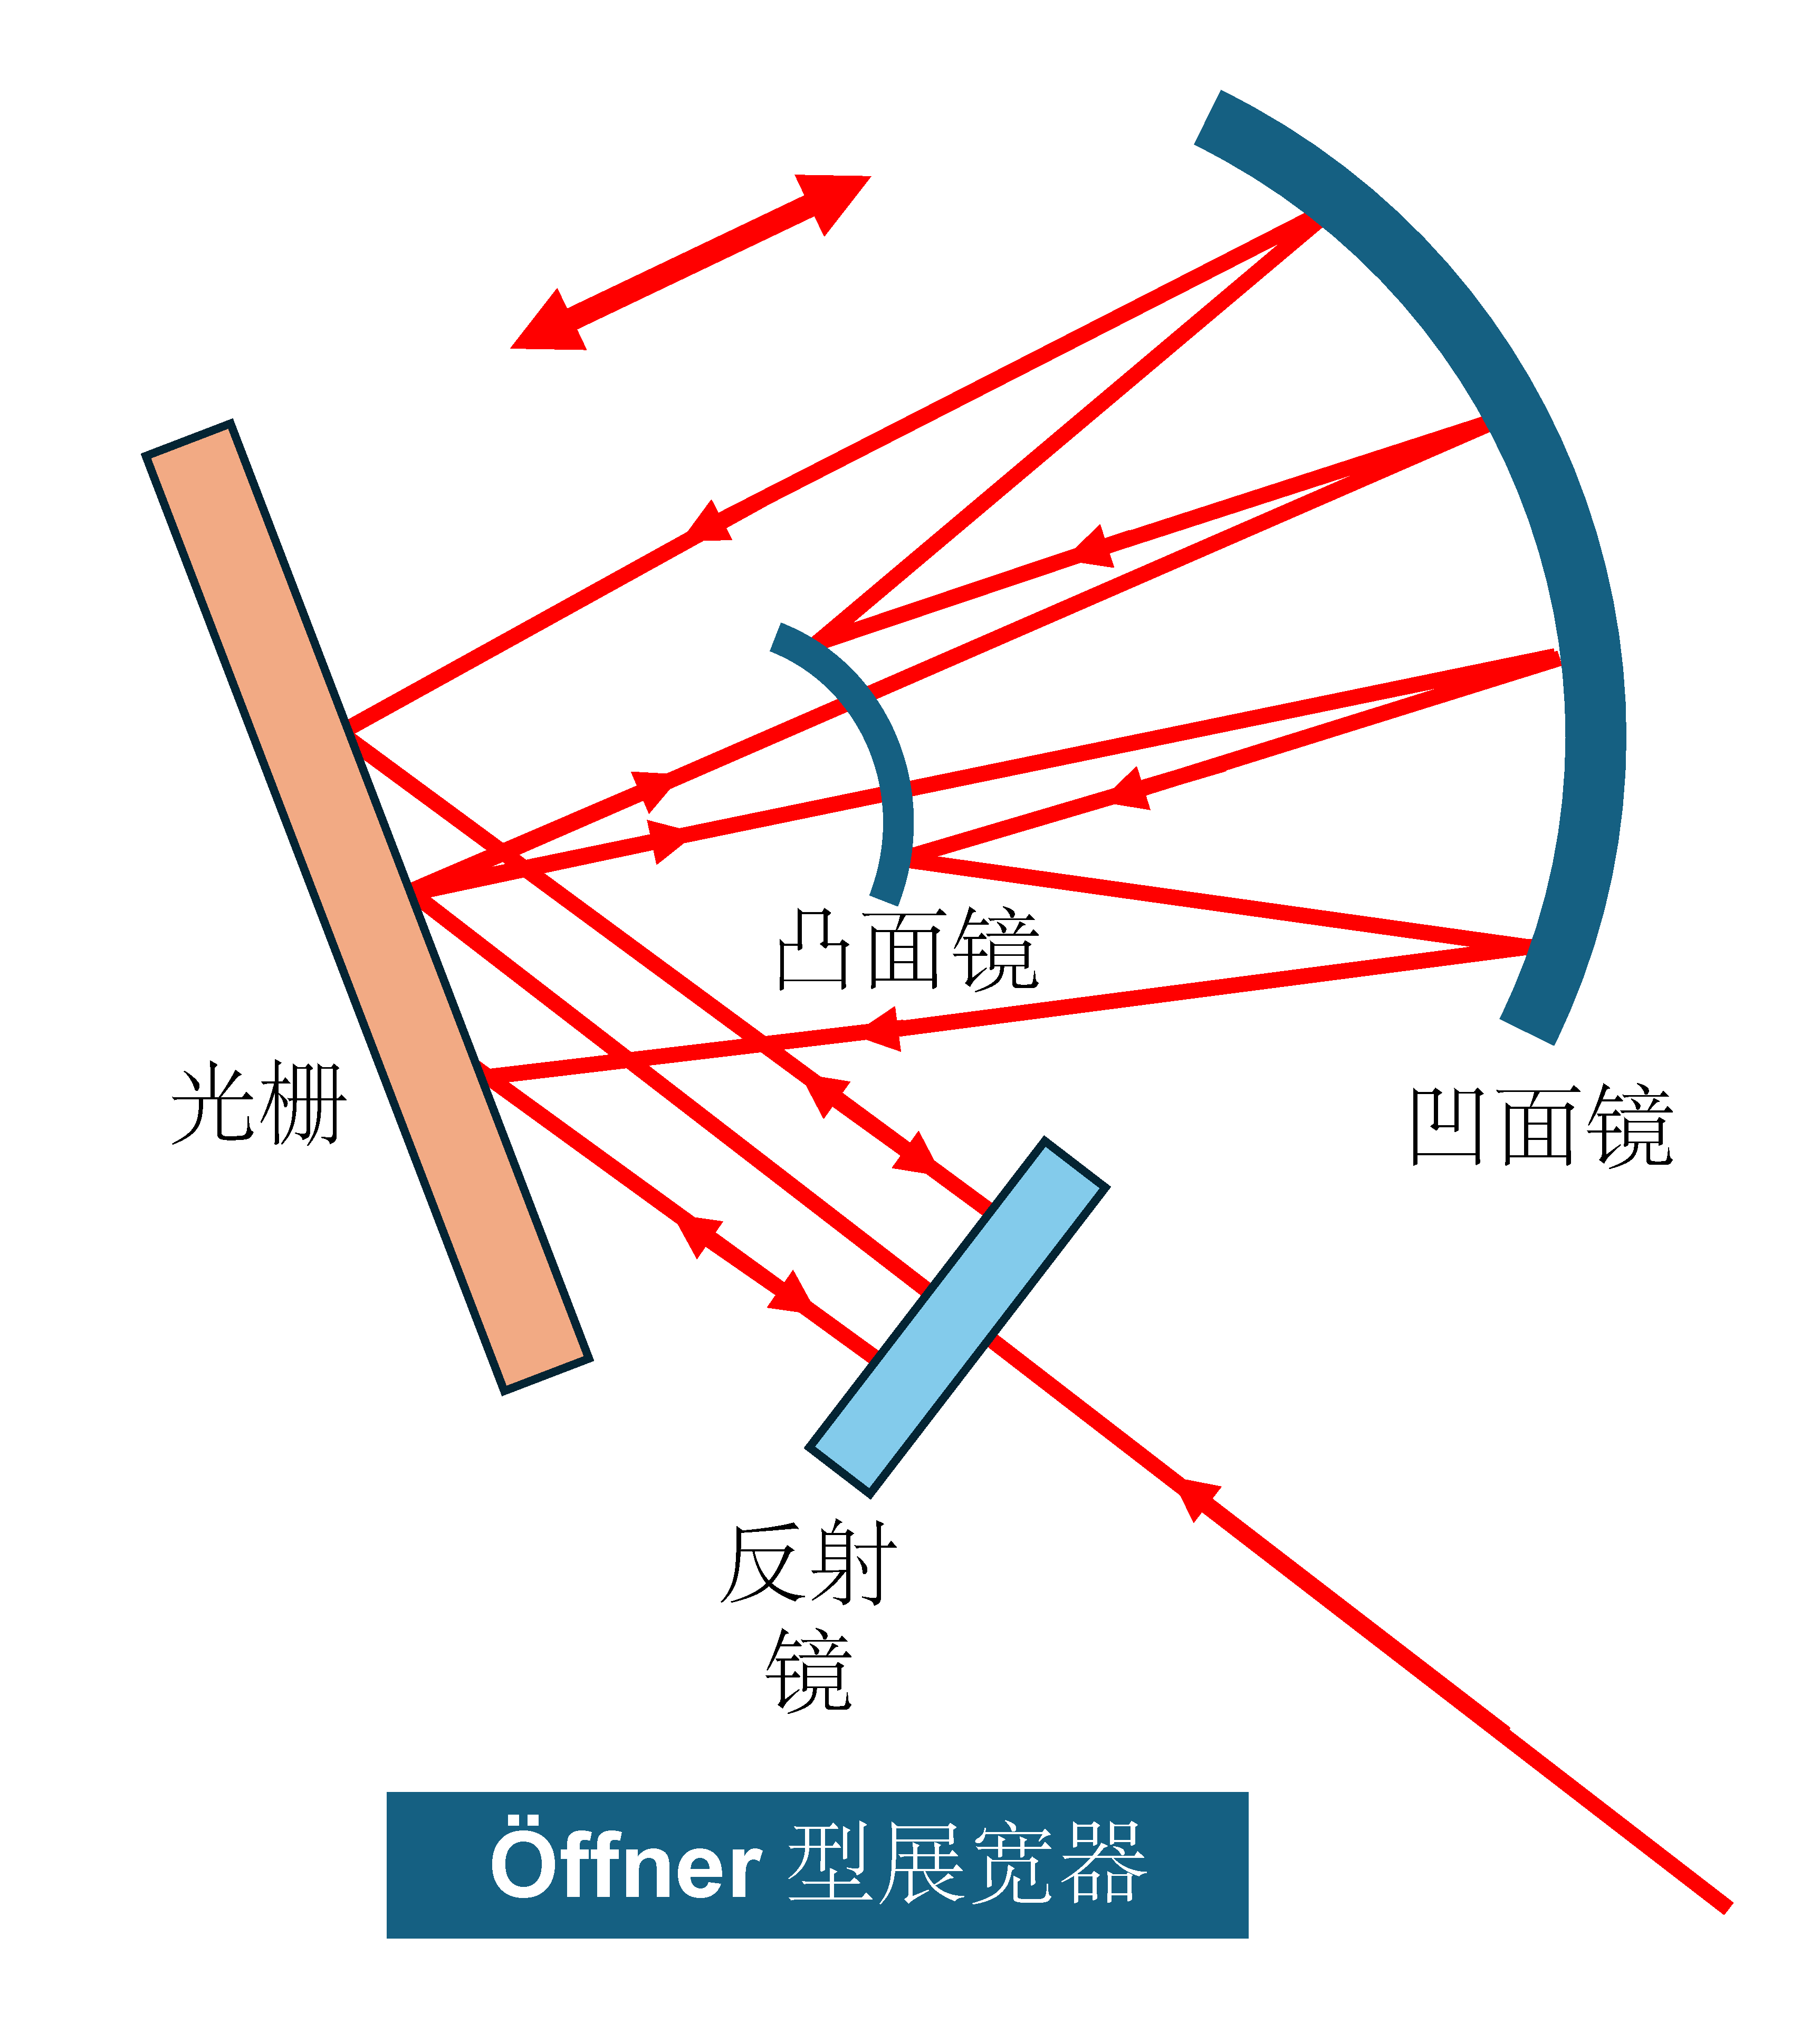
\includegraphics[width=\textwidth]{Fig/FigGrating-1.pdf}
        \caption{}
        \label{fig:grating_compare_a}
    \end{subfigure}
    \hfil
    \begin{subfigure}[b]{0.31\textwidth}
        \centering
        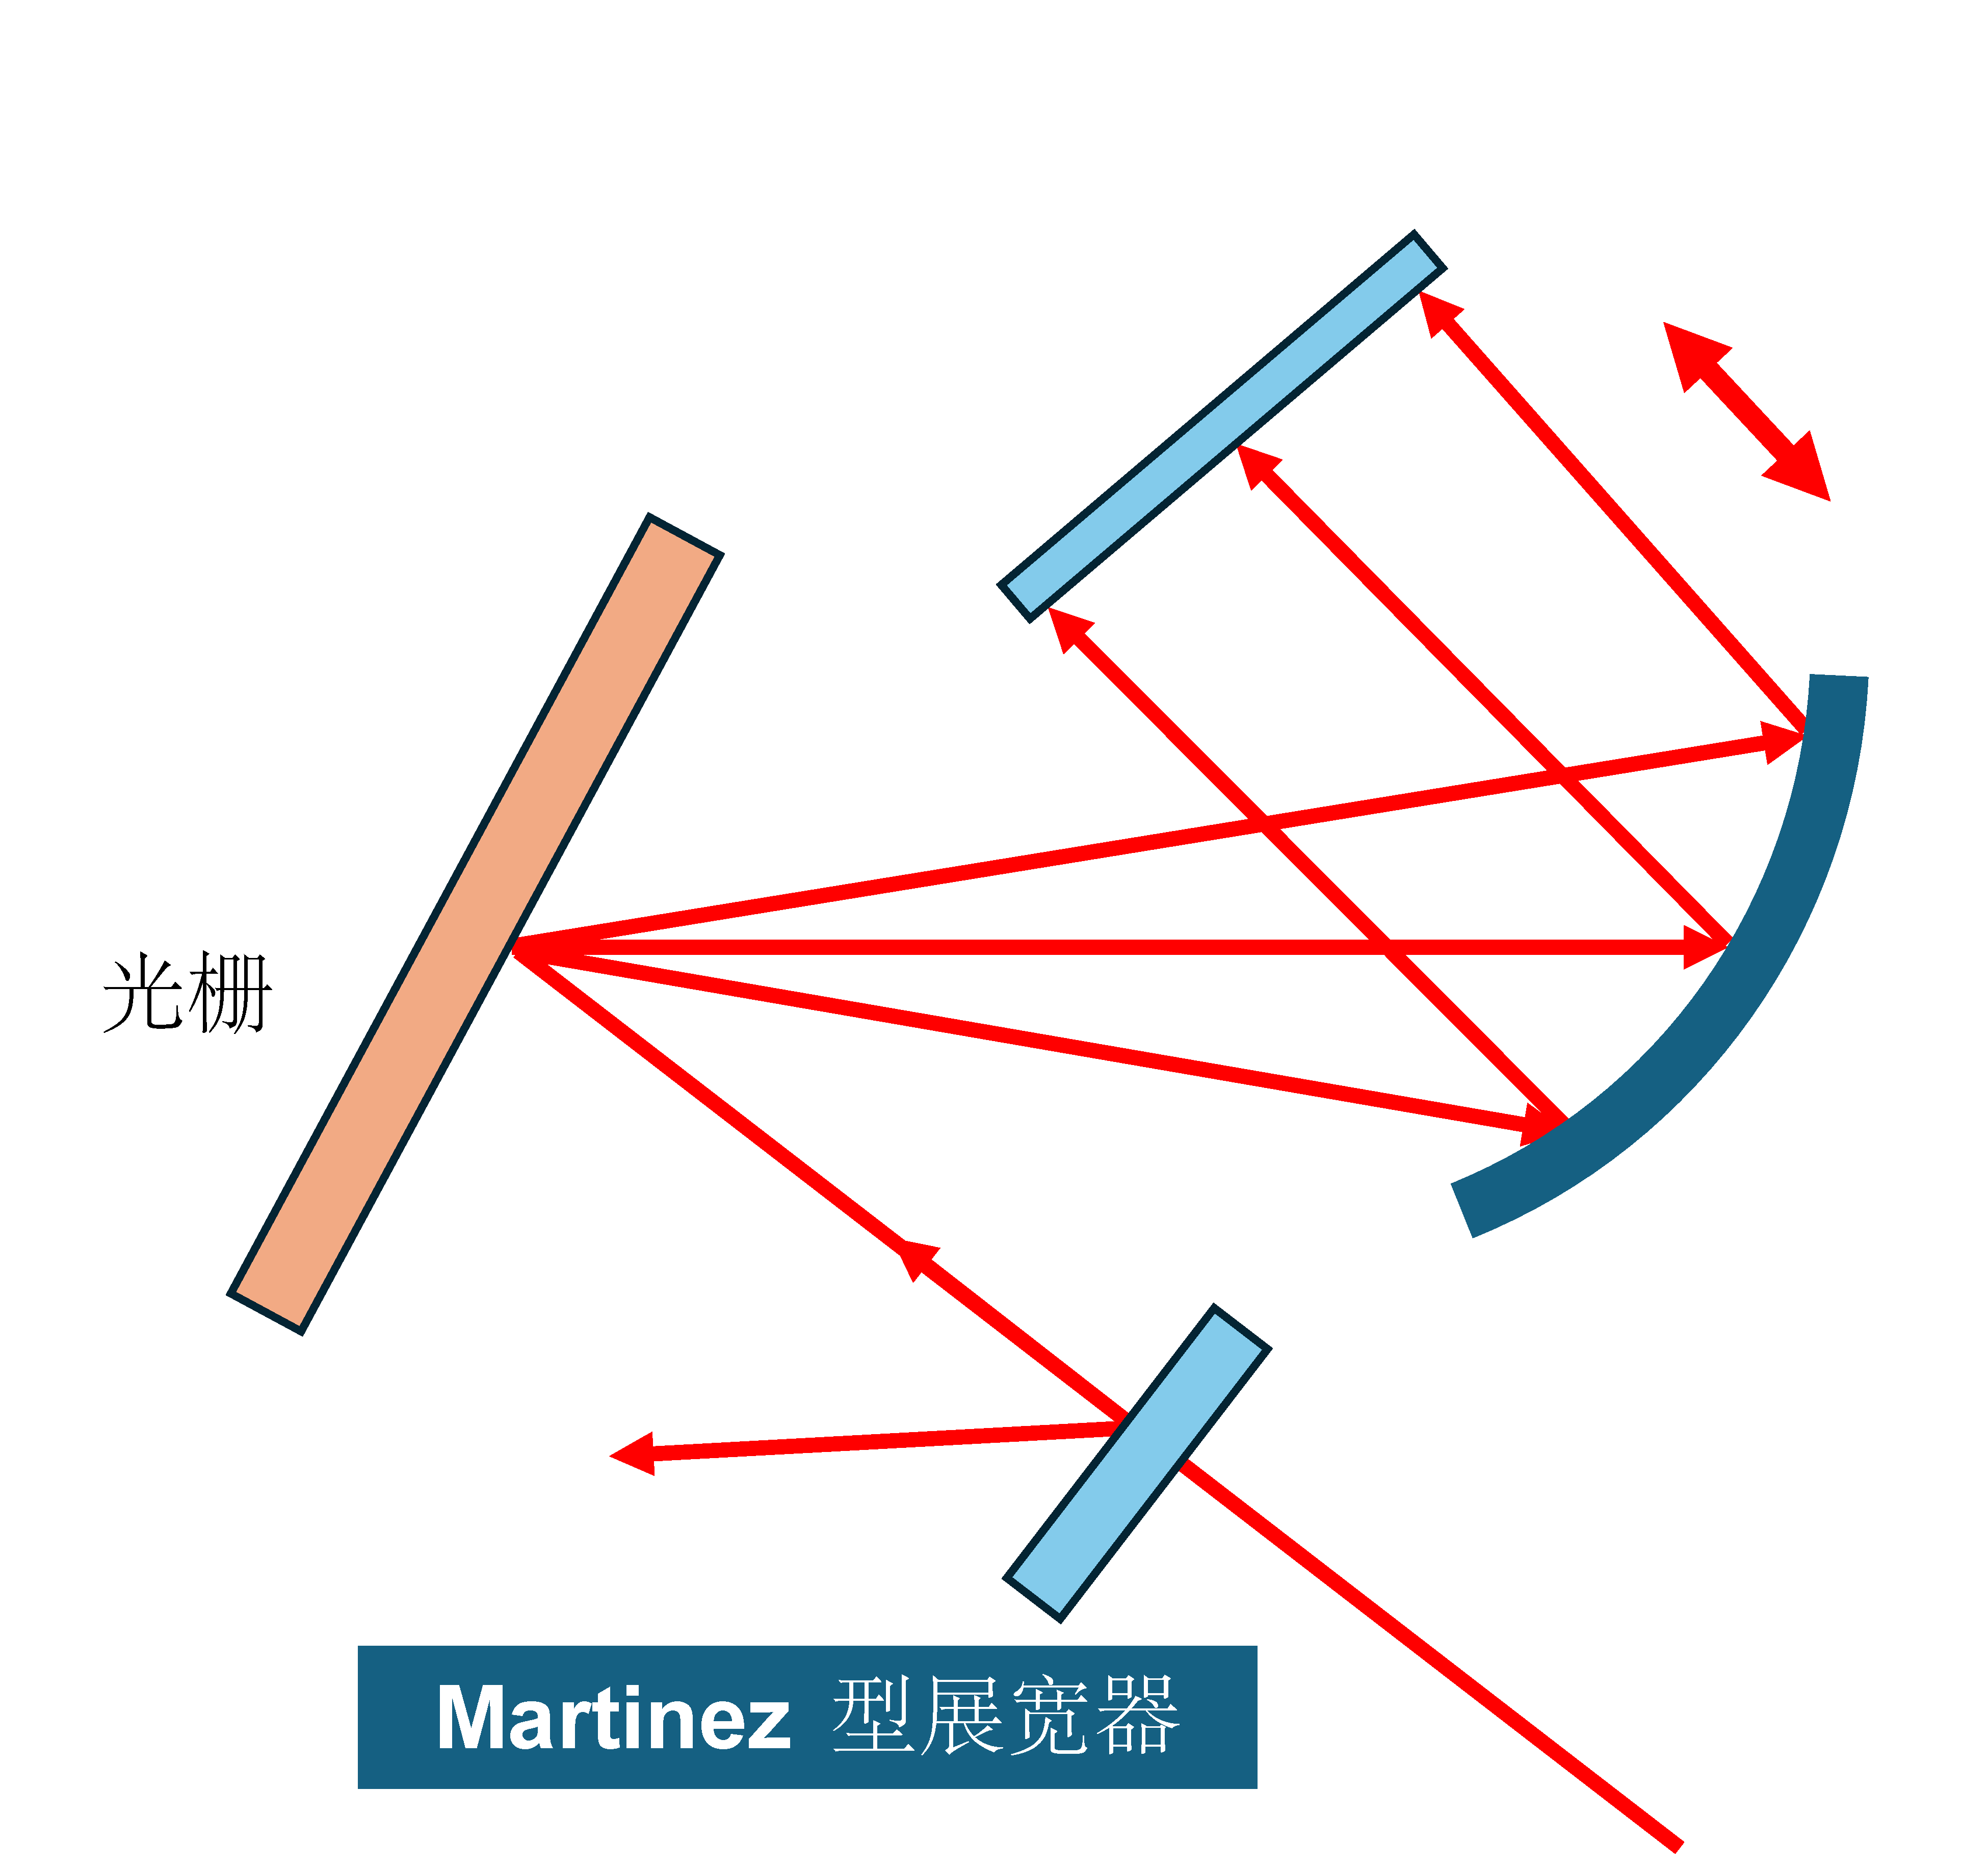
\includegraphics[width=\textwidth]{Fig/FigGrating-2.pdf}
        \caption{}
        \label{fig:grating_compare_b}
    \end{subfigure}
    \hfil
    \begin{subfigure}[b]{0.33\textwidth}
        \centering
        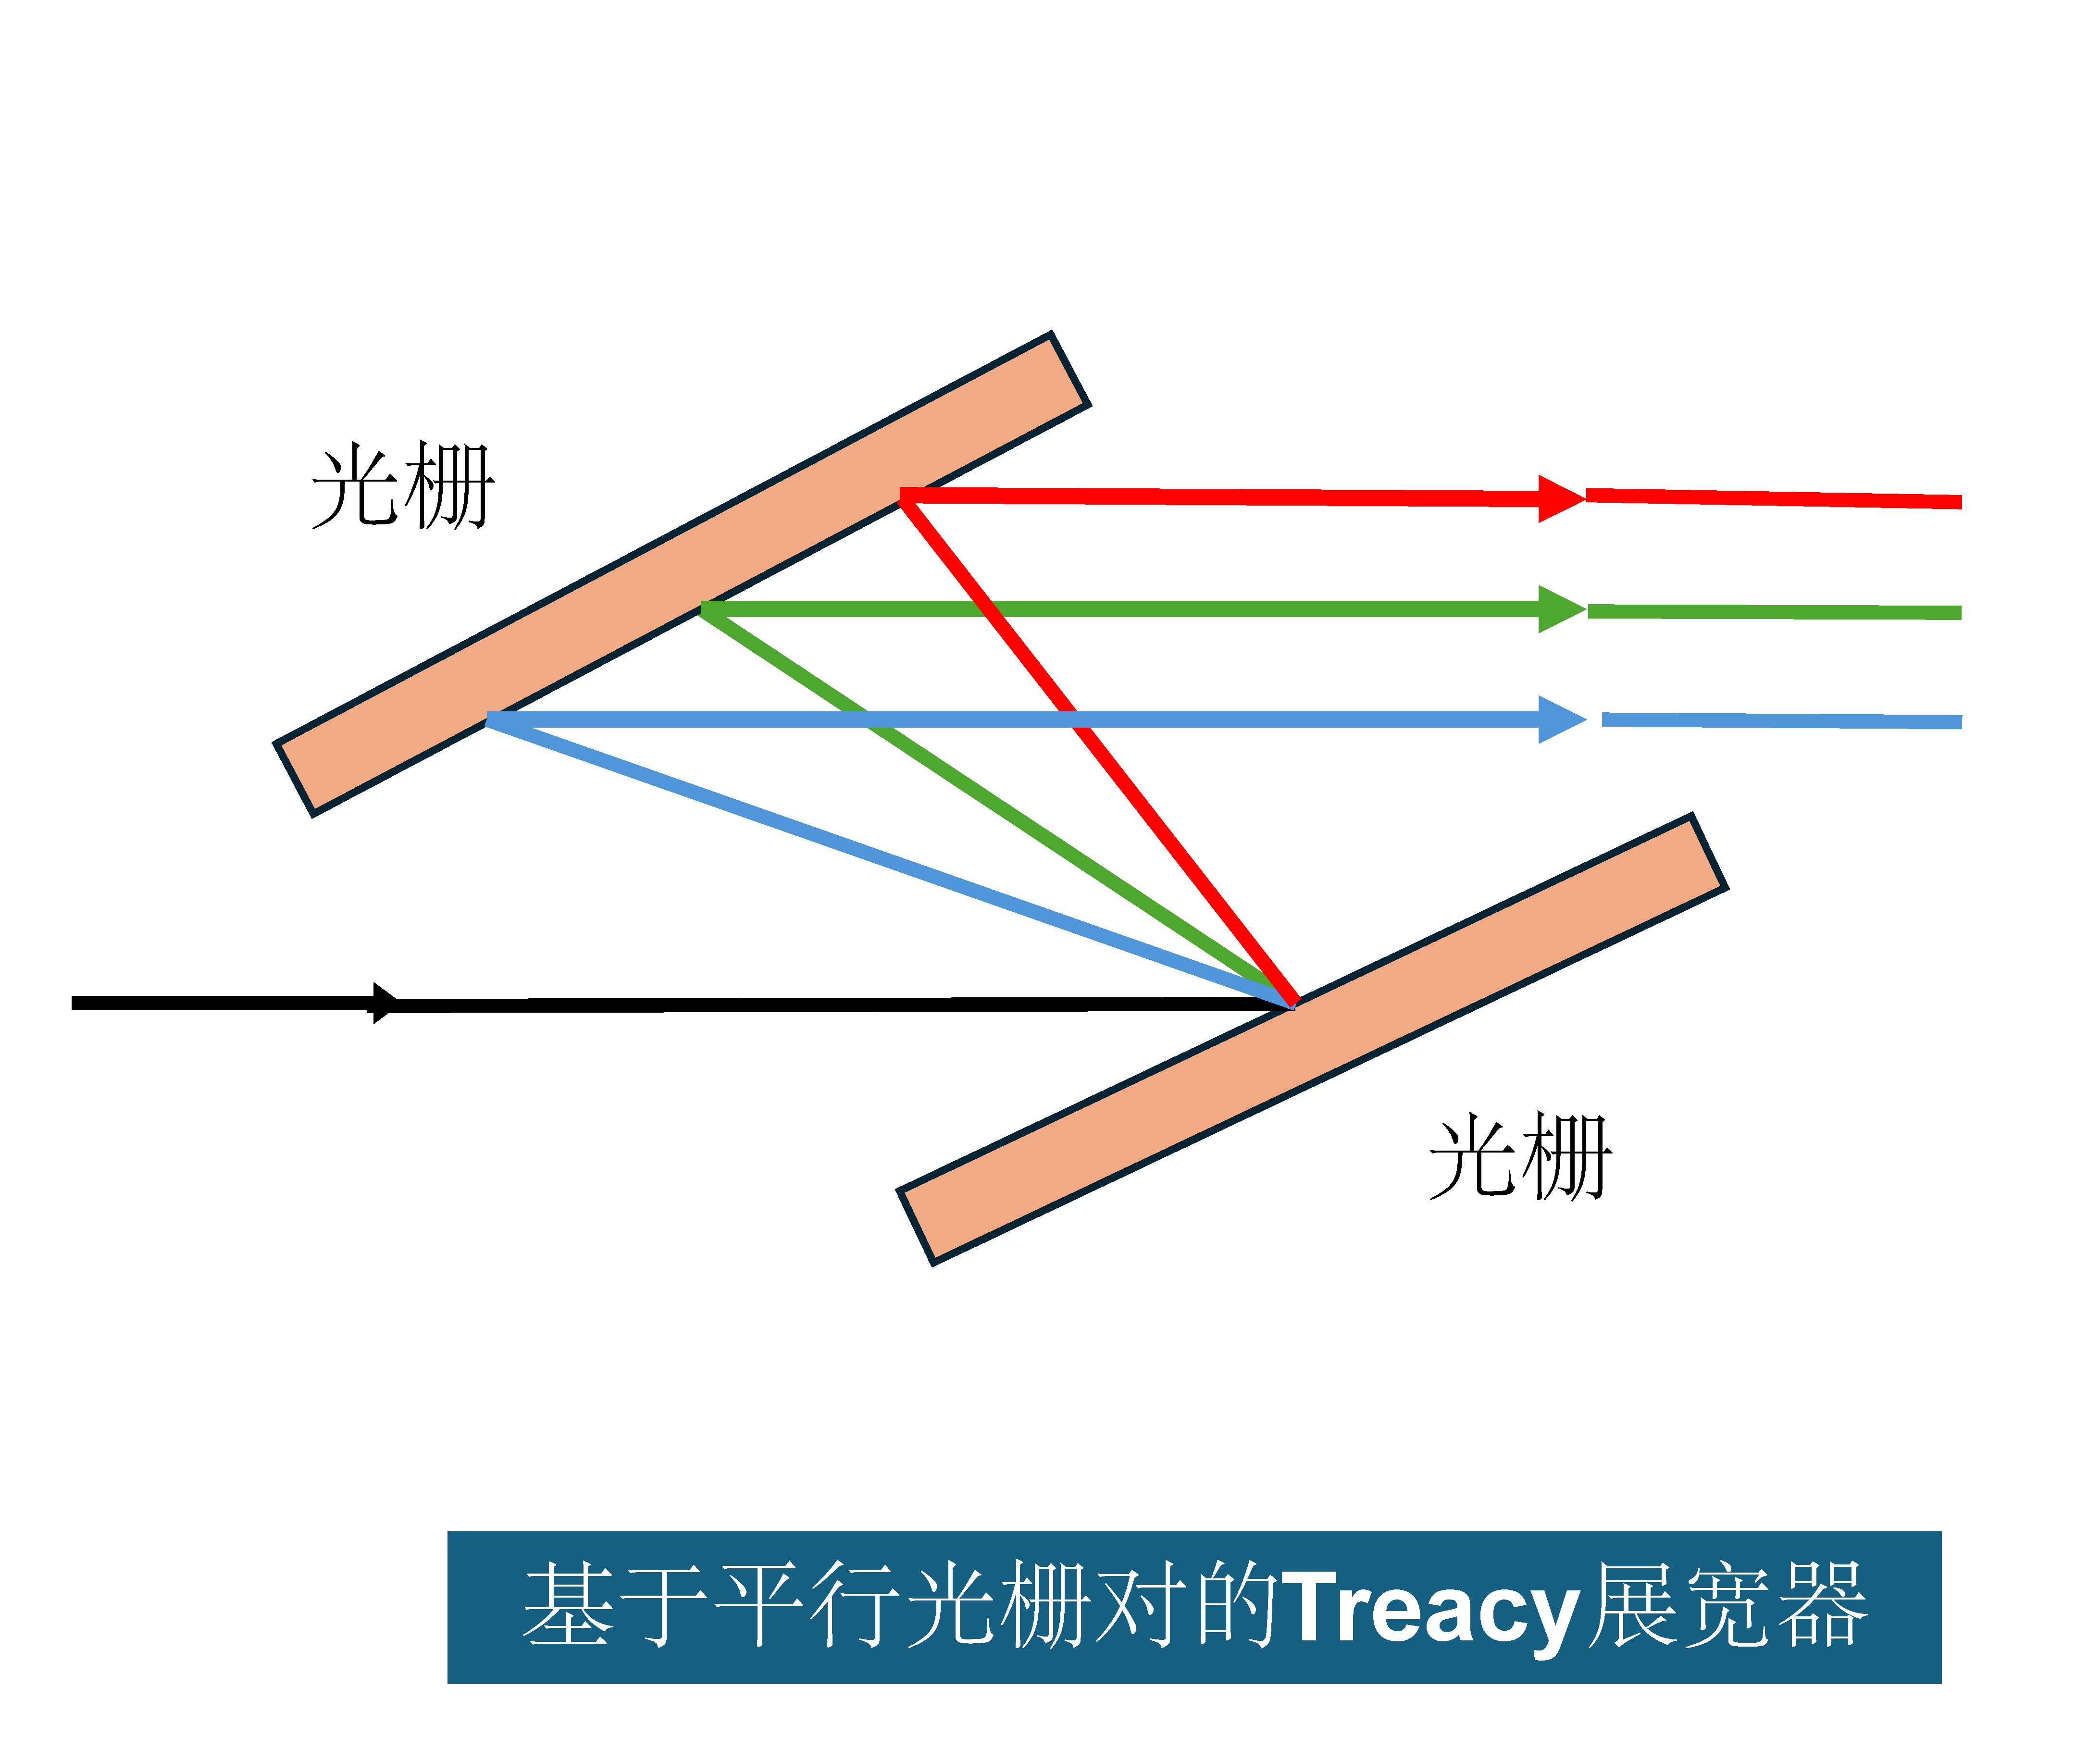
\includegraphics[width=\textwidth]{Fig/FigGrating-3.pdf}
        \caption{}
        \label{fig:grating_compare_c}
    \end{subfigure}
    \bicaption{三种典型光栅展宽器结构示意图。(a)Öffner 型展宽器；(b)Martinez 型展宽器；(c)基于平行光栅对的 Treacy 展宽器}
    {Schematic comparison of three typical grating-based stretchers. (a) Öffner stretcher; (b) Martinez stretcher; (c) Treacy stretcher based on a parallel grating pair}
    \label{fig:grating_compare}
\end{figure}

如图~\ref{fig:grating_compare}所示，图~\ref{fig:grating_compare}(\subref{fig:grating_compare_a}) 为 Öffner 型展宽器，其特点是在折返光路中引入凹面镜与凸面镜组合，从而在较紧凑的空间内实现色散管理；图~\ref{fig:grating_compare}(\subref{fig:grating_compare_b}) 为 Martinez 型展宽器，该结构通过光栅与成像镜组配合，可在较灵活的参数条件下实现脉冲展宽与压缩；图~\ref{fig:grating_compare}(\subref{fig:grating_compare_c}) 为基于平行光栅对的 Treacy 型展宽器，其结构相对直观，是最经典的光栅色散补偿方案之一。总体而言，光栅类方案通常具有较强的色散调节能力，但其系统体积、插入损耗以及对准复杂度相对较高。

对于本文所搭建的 920 nm 多光子显微系统而言，系统更关注预补偿结构的可调性、透过效率以及实验搭建的简洁性。因此，尽管光栅展宽器在大色散补偿场景中具有明显优势，但综合系统复杂度与实验实现难度后，本文并未采用光栅类方案作为主要预补偿结构，而是进一步选择棱镜对方案完成后续色散补偿设计与实验优化。



\subsection{基于棱镜对的 920\,nm 飞秒激光脉冲压缩}\label{4.5.2}

\begin{figure}[htbp]
    \centering
    \begin{subfigure}[b]{0.55\textwidth}
        \centering
        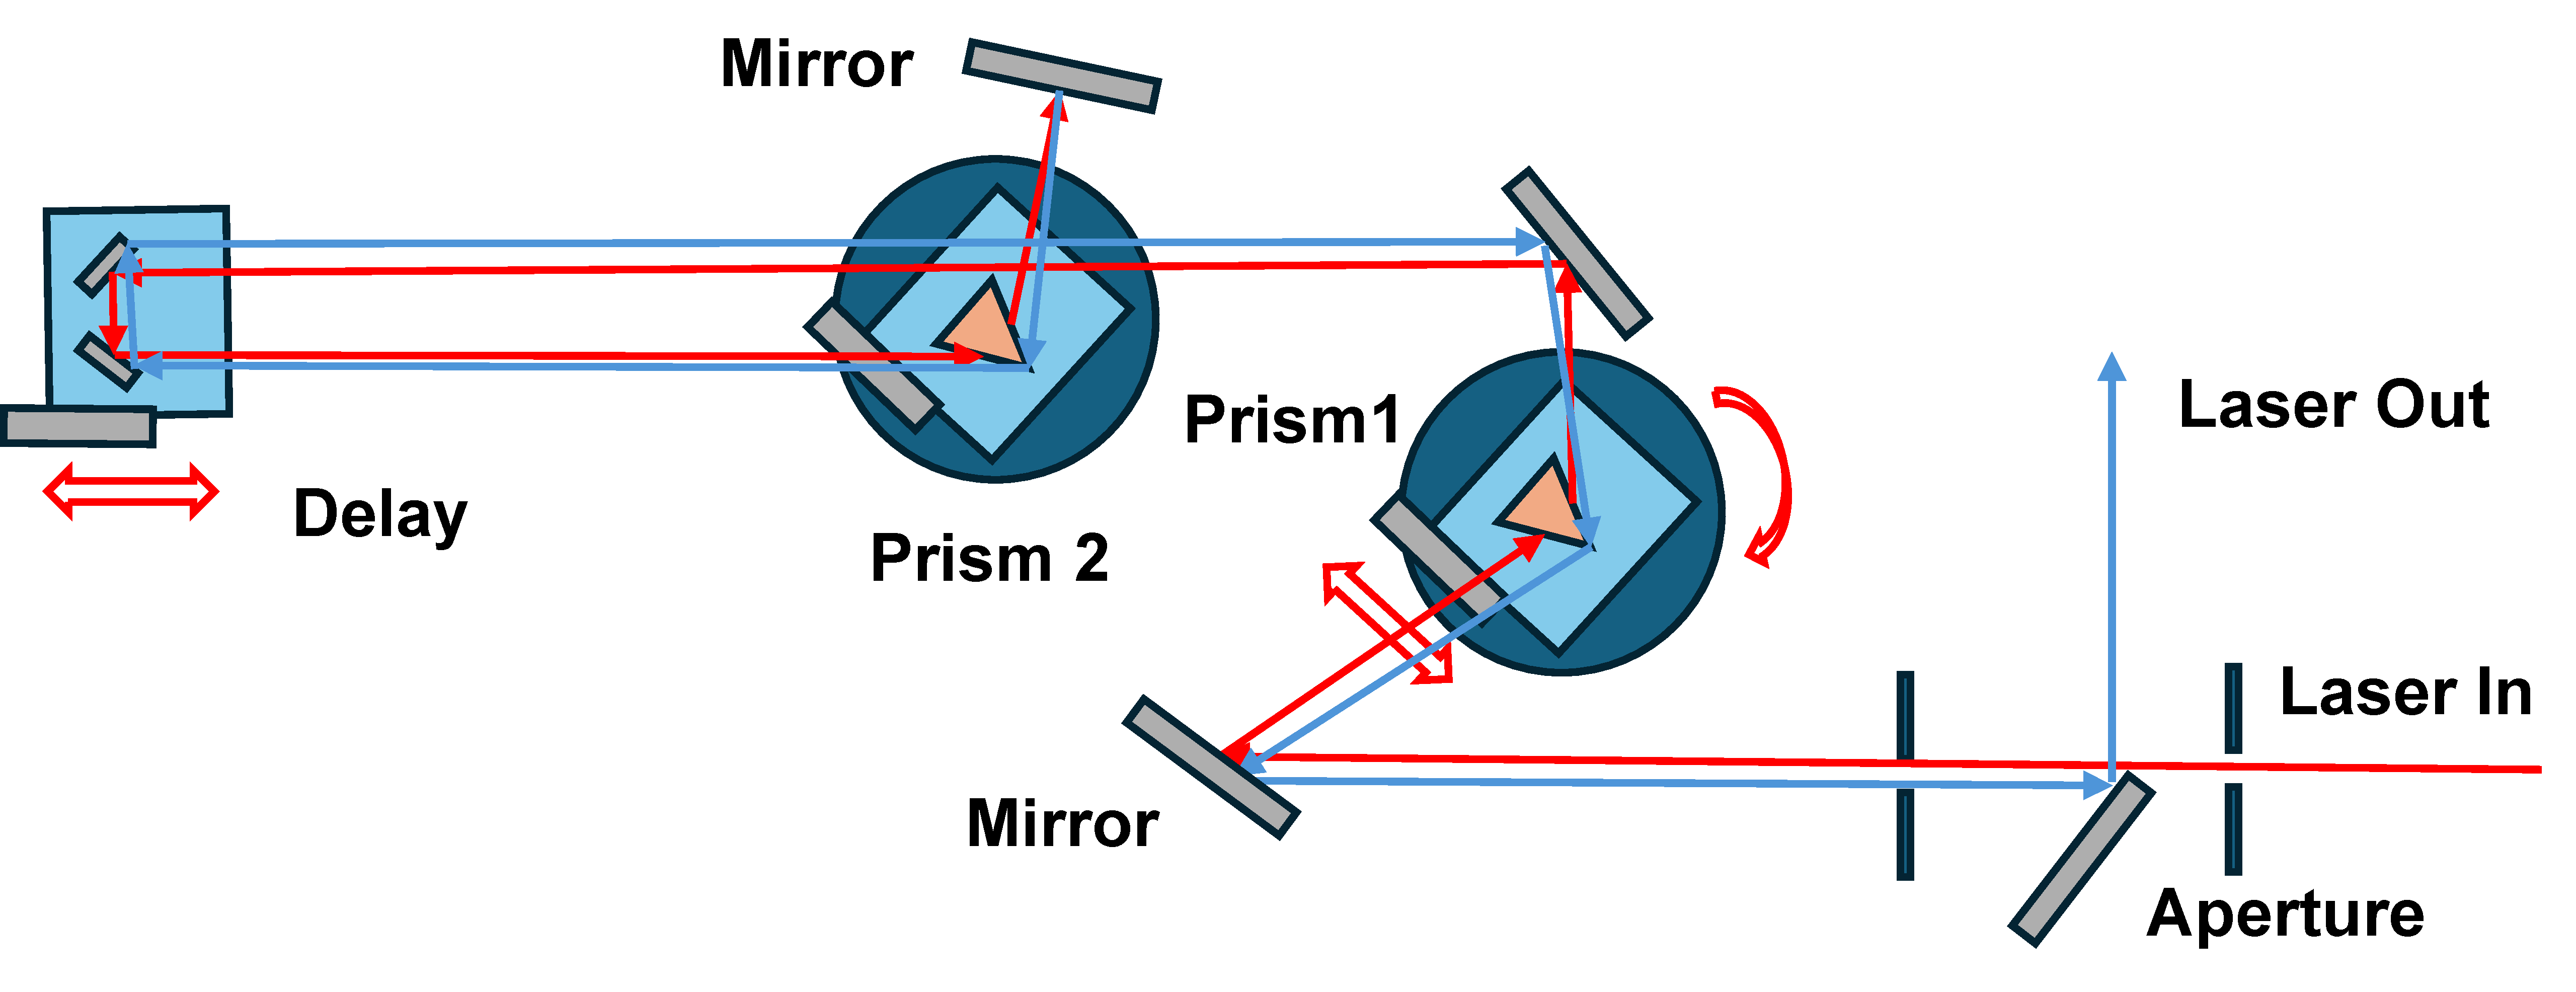
\includegraphics[width=\textwidth]{Fig/Fig11.pdf}
        \caption{}
        \label{fig11}
    \end{subfigure}
    \vspace{0.3cm}
    \begin{subfigure}[b]{0.35\textwidth}
        \centering
        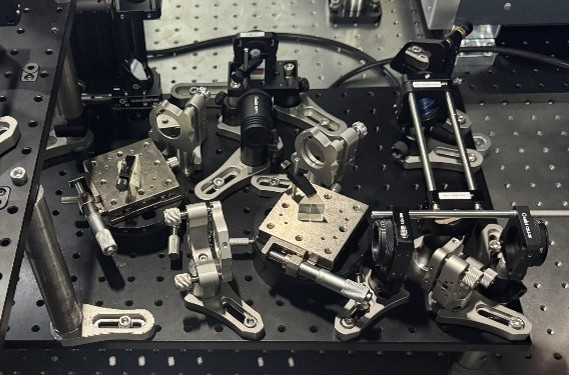
\includegraphics[width=\textwidth]{Fig/Fig12.jpg}
        \caption{}
        \label{fig12}
    \end{subfigure}
    \bicaption{针对 920\,nm 飞秒激光器设计的双棱镜脉冲压缩装置。(a) 棱镜对压缩器光路示意图；(b) 压缩器实拍图}{Prism-pair pulse compressor designed for a 920\,nm femtosecond laser. (a) Optical layout of the prism-pair compressor; (b) photograph of the compressor}
    \label{fig11-12}
\end{figure}

针对本文多光子成像系统中的 920\,nm 双光子激发通道，本文在腔外搭建了一套独立的棱镜对脉冲压缩器。该压缩器的作用是在激光进入显微系统之前预先引入可调的负色散，以补偿后续扫描光学、物镜以及其他光学元件带来的正色散累积，从而使激光在样品处重新获得更短脉宽和更高峰值功率。

在棱镜材料的选择上，本文优先考虑近红外波段具有较强色散能力、市场上易于采购且加工成熟的光学玻璃。综合材料折射率、色散特性以及实际可获得性后，最终选用 N-SF11 玻璃作为棱镜材料。棱镜对压缩器通常采用等边三棱镜结构，并使激光以接近布儒斯特角的条件入射到棱镜表面，以减小 $p$ 偏振光在界面上的反射损耗，提高系统整体透过效率。对于 N-SF11 材料，其在近红外波段的布儒斯特角接近 $60^\circ$，因此本文采用近布儒斯特角入射方式进行设计，以兼顾较高透射效率与较好的色散调节能力。

需要说明的是，布儒斯特角设计并不是为了``获得最大色散''，而是为了在保证色散调节能力的同时尽量降低 $p$ 偏振光的 Fresnel 反射损耗。对于多光子显微系统，由于激发光在经过压缩器、扫描系统和物镜后还要继续损耗，因此压缩器本身的通光效率具有重要意义。采用近布儒斯特角入射，可以显著减小界面反射，提高压缩器的整体输出效率。

如图~\ref{fig11-12}(\subref{fig11}) 所示，激光首先经光阑准直后进入系统，通过反射镜以接近布儒斯特角的方式入射到第一个 N-SF11 等边色散棱镜上，在棱镜中引入角色散和材料色散；随后激光经反射镜与可调延迟线传播后，以相似入射条件进入第二个棱镜，再经反射镜系统折返返回输出端，最终重新耦合回显微系统主光路。整个装置的关键可调参数包括棱镜插入深度以及两棱镜之间的相对间距，这两个参数共同决定压缩器所引入的总色散。

在压缩器回程设计中，需要特别注意反射镜构型对光路高度与输出稳定性的影响，如图\ref{FigSup2-4}。部分文献在第二个棱镜后采用单反射镜回折方案，这种结构虽然较为简单，但在调节延迟线时容易导致返回光路高度发生变化，从而引起后续系统耦合不稳定和输出功率波动。如图~\ref{FigSup2-4}(\subref{FigSup02}) 和图~\ref{FigSup2-4}(\subref{FigSup03}) 所示，单反射镜方案在调节过程中会带来明显的光路高度变化及功率变化。因此，本文采用双反射镜回程设计，以尽可能保持光路高度恒定并提高压缩器输出稳定性。

\begin{figure}[htbp]
    \centering
    \begin{subfigure}{0.47\linewidth}
        \centering
        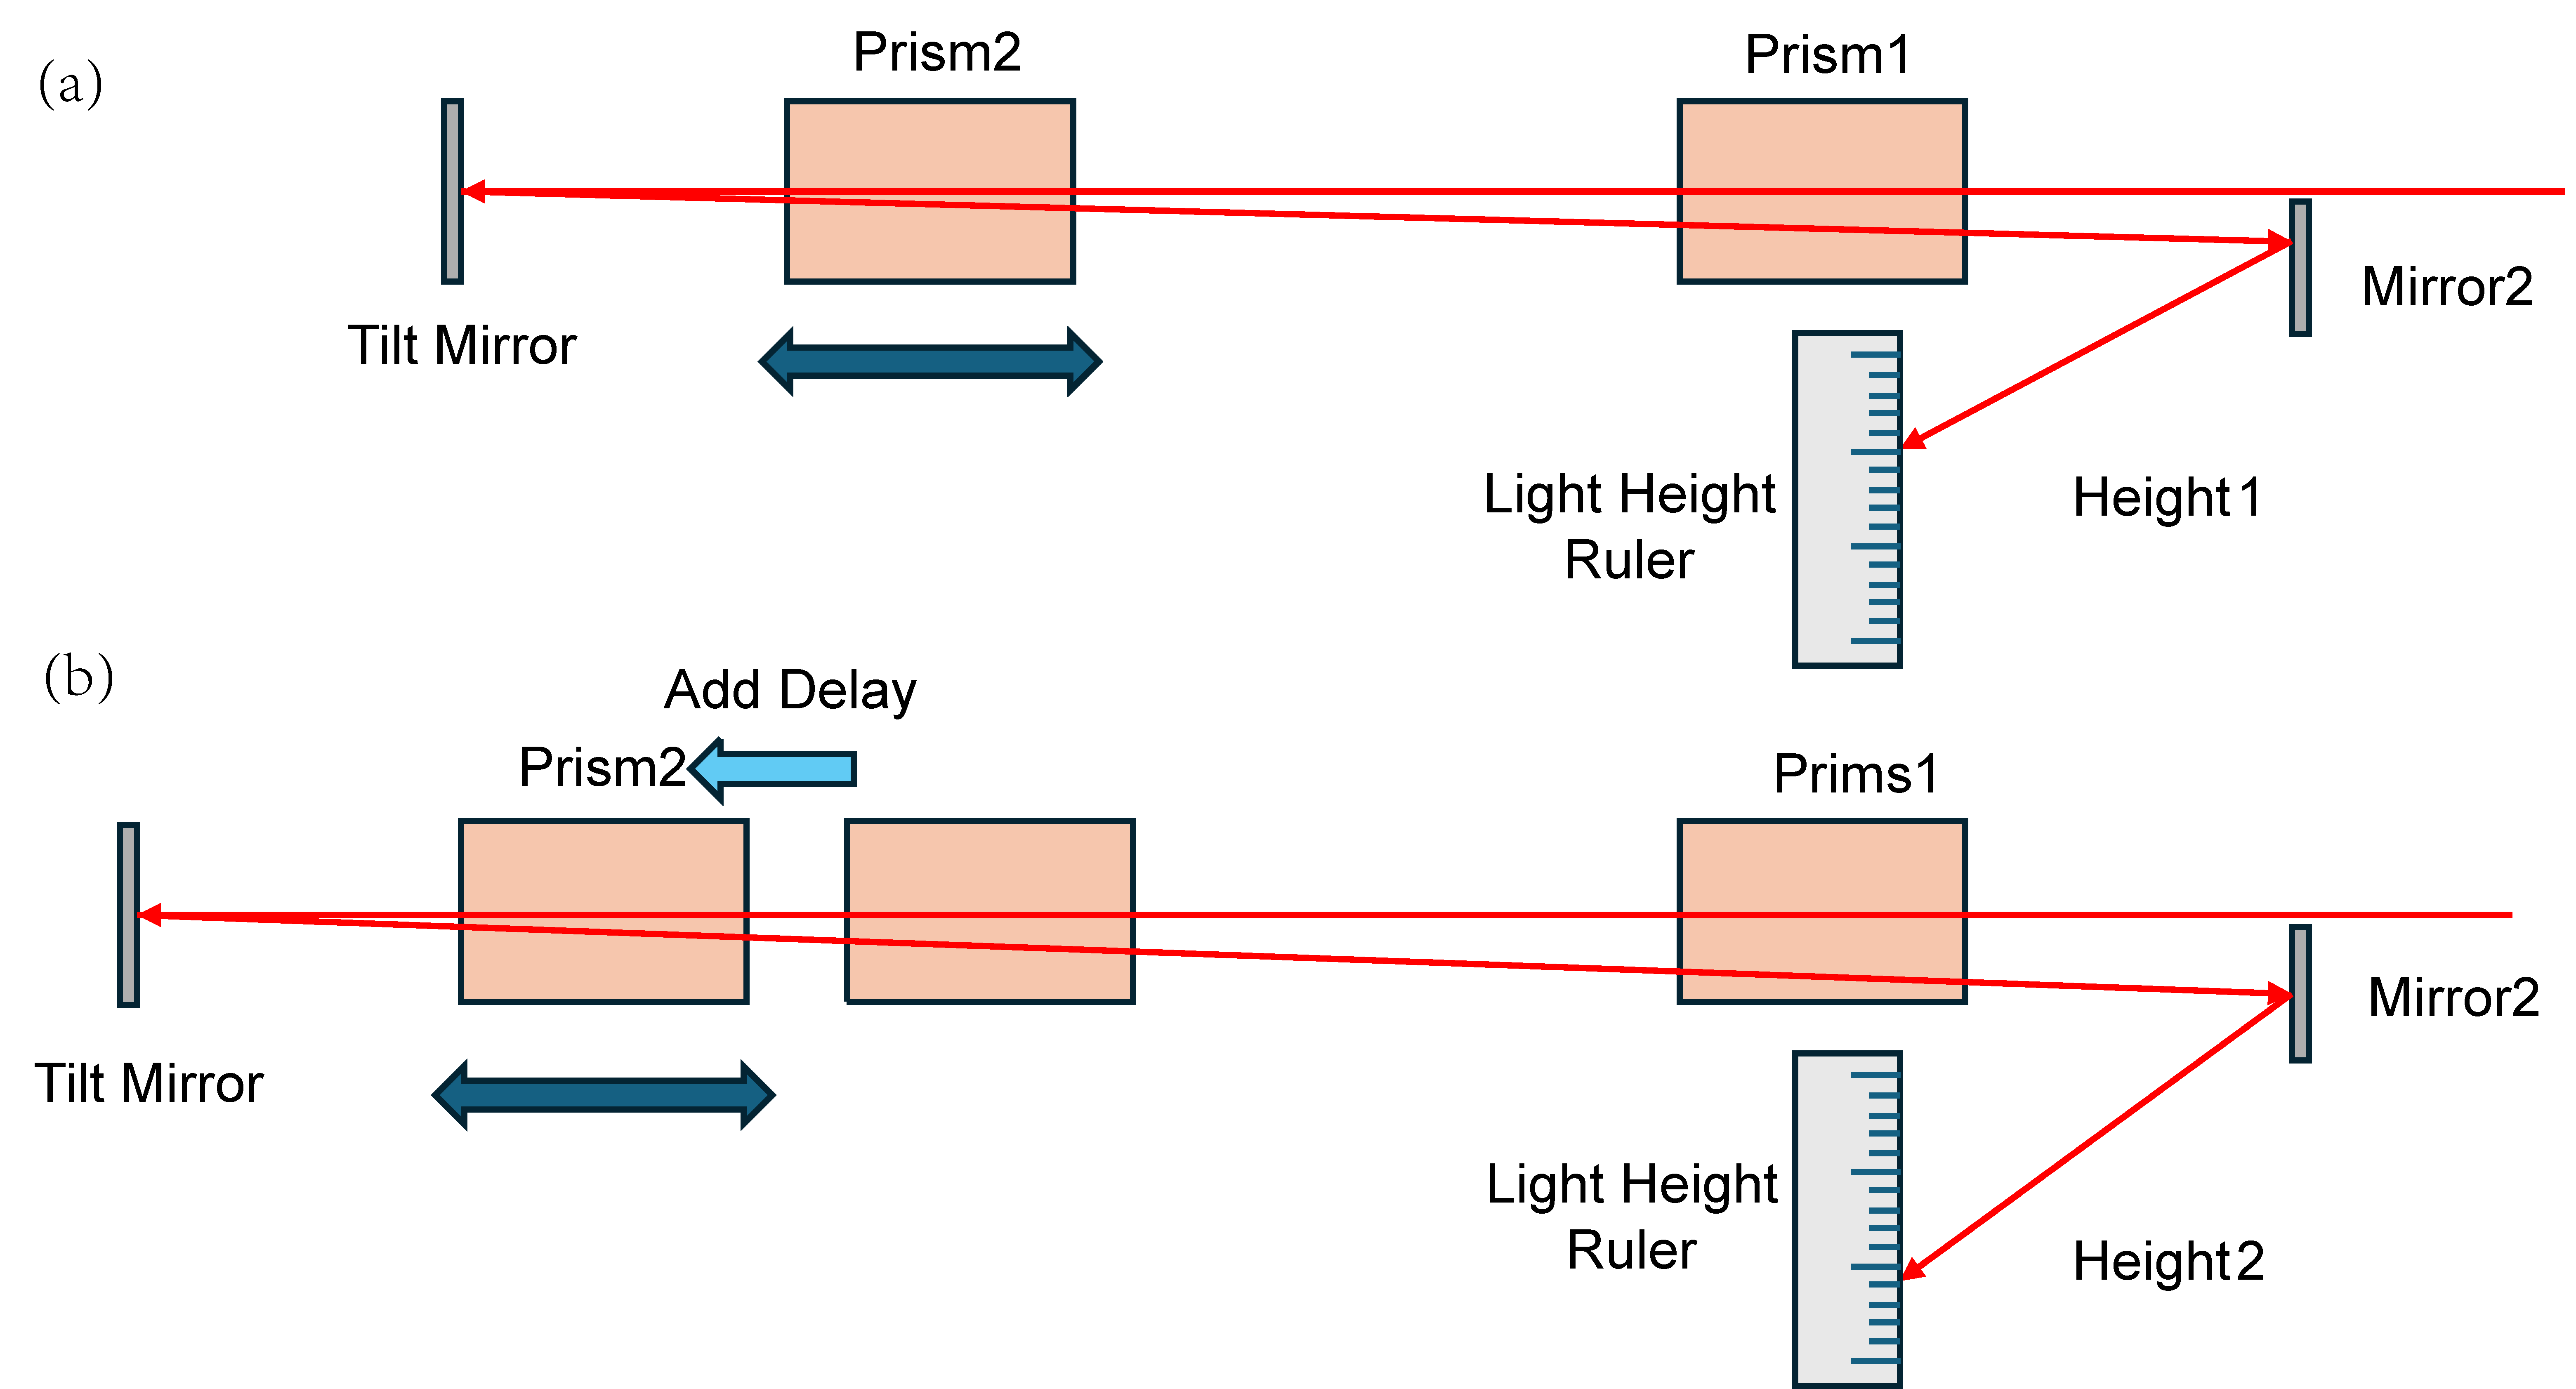
\includegraphics[width=\linewidth]{Fig/FigSup02.pdf}
        \caption{}
        \label{FigSup02}
    \end{subfigure}%
    \hspace{0.03\linewidth}%
    \begin{subfigure}{0.38\linewidth}
        \centering
        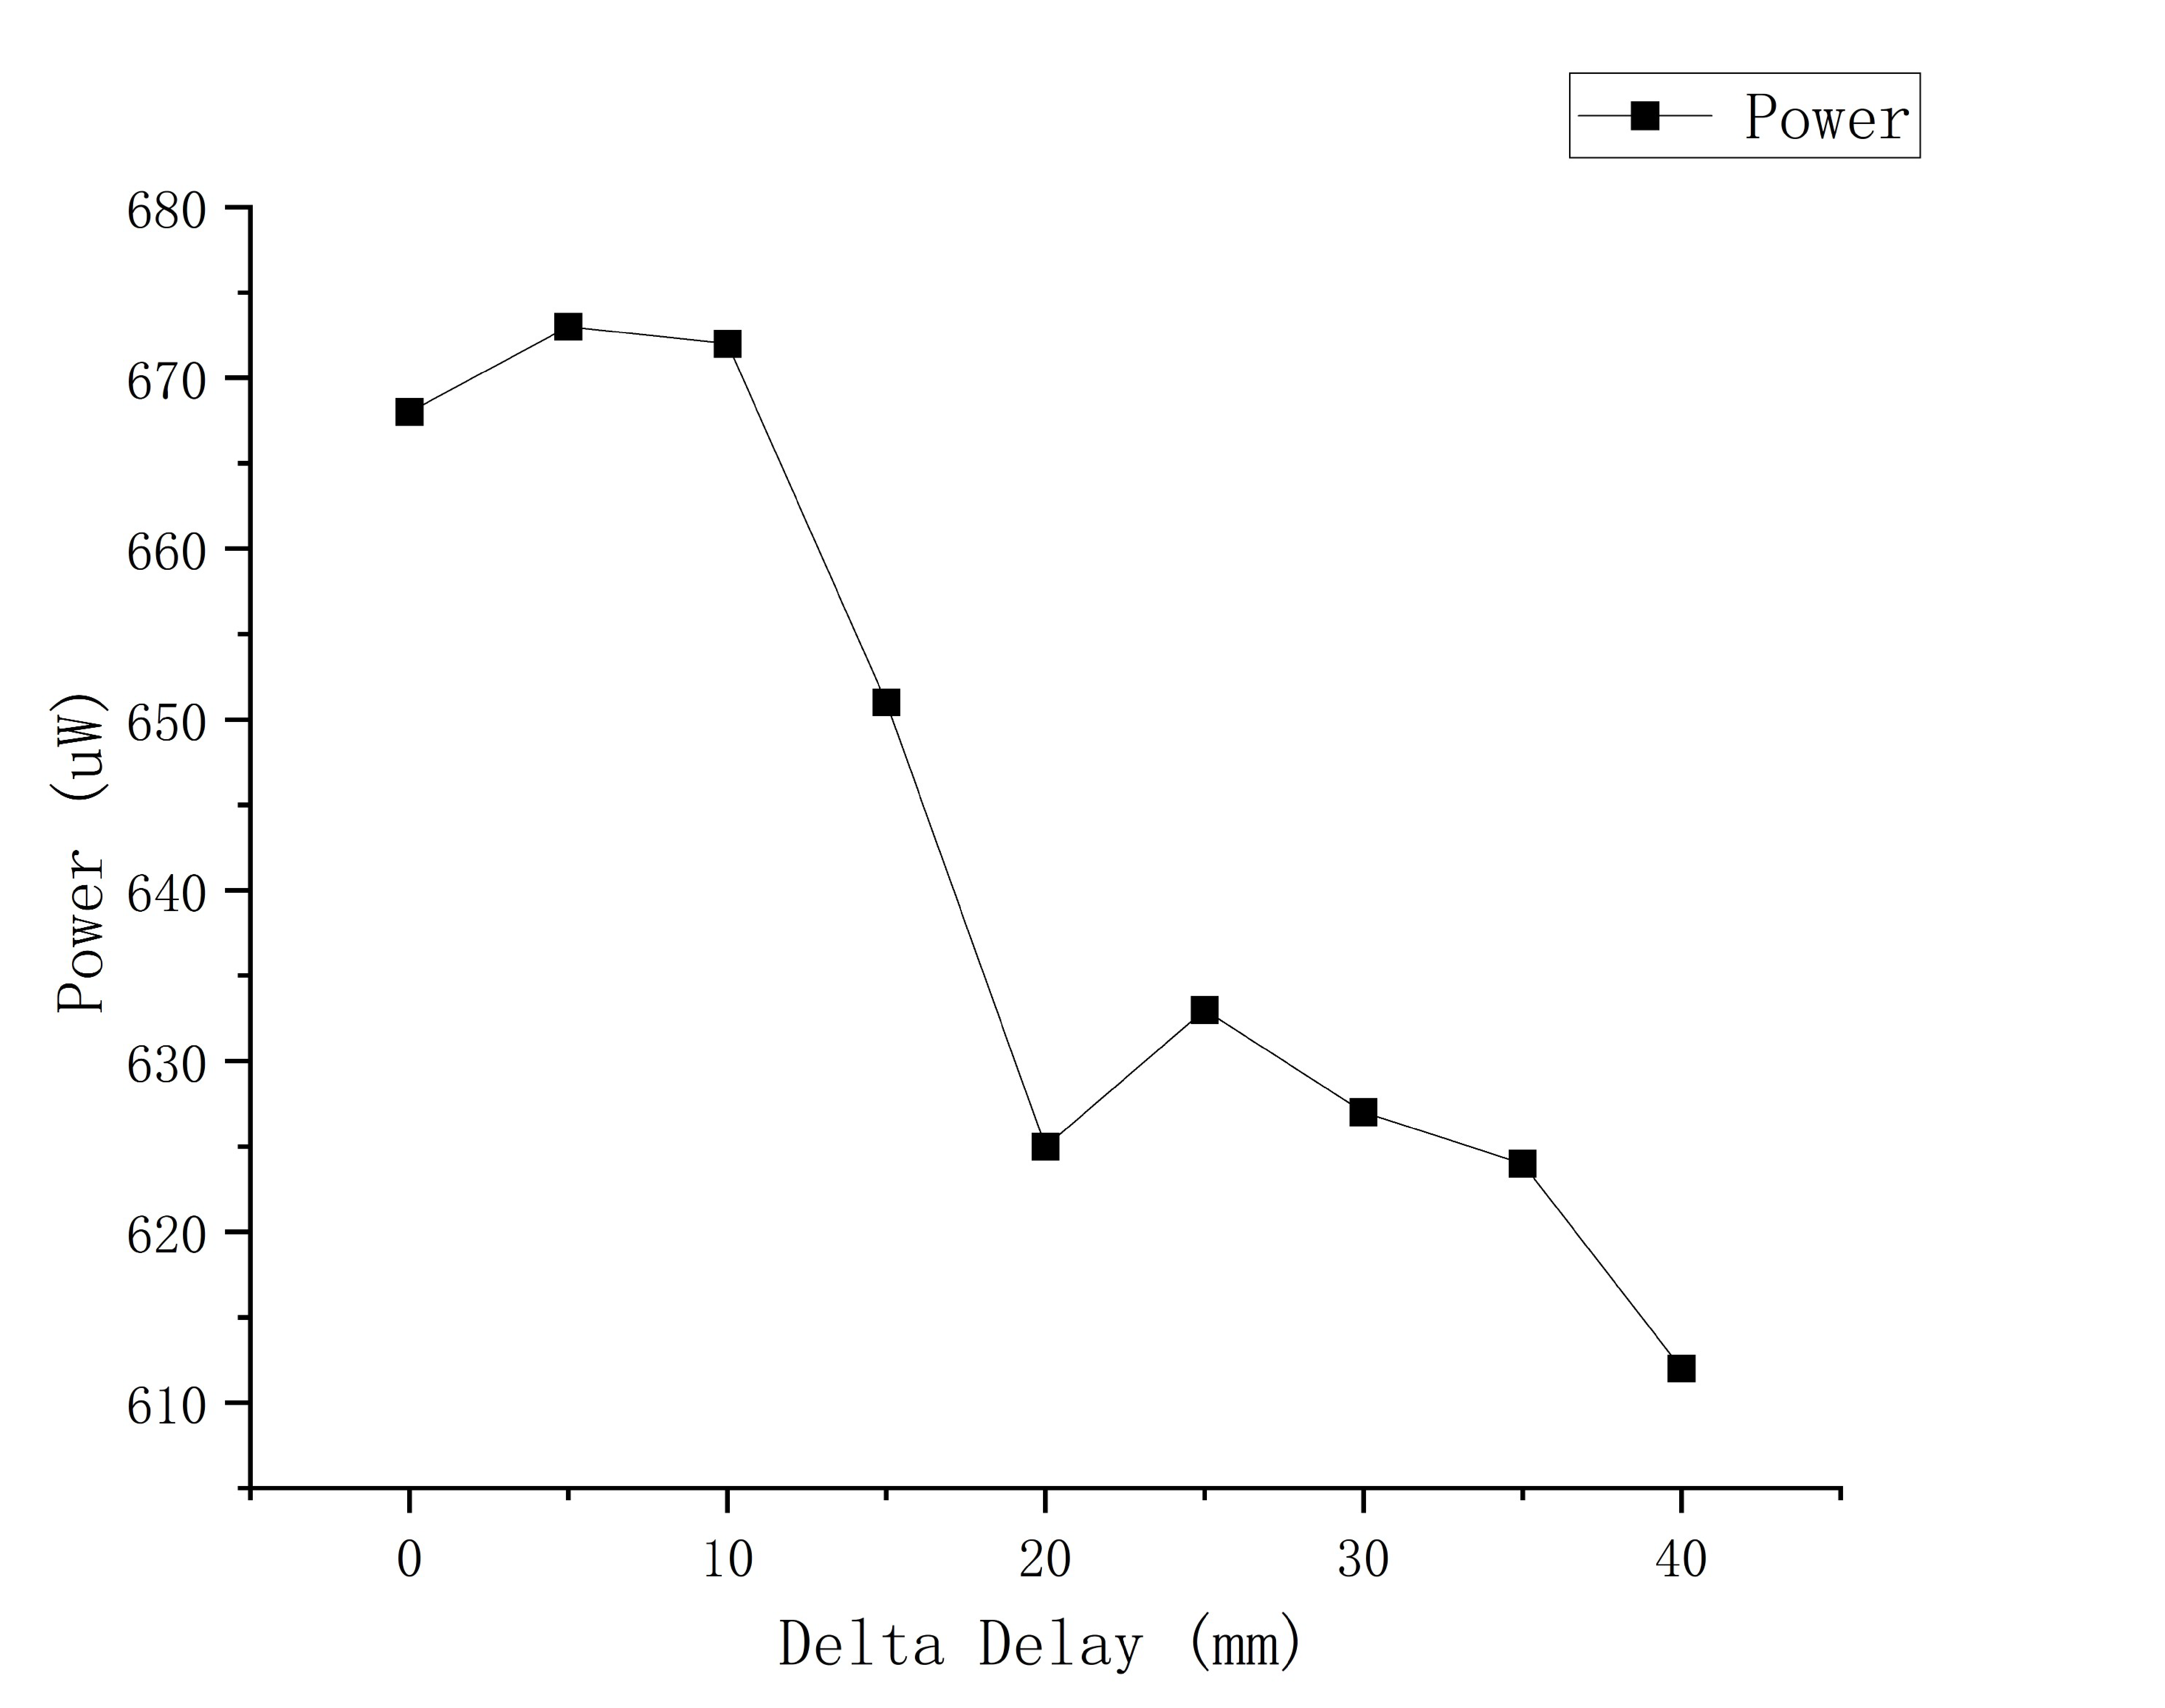
\includegraphics[width=\linewidth]{Fig/FigSup03.pdf}
        \caption{}
        \label{FigSup03}
    \end{subfigure}
    \vspace{1em}
    \begin{subfigure}{0.9\linewidth}
        \centering
        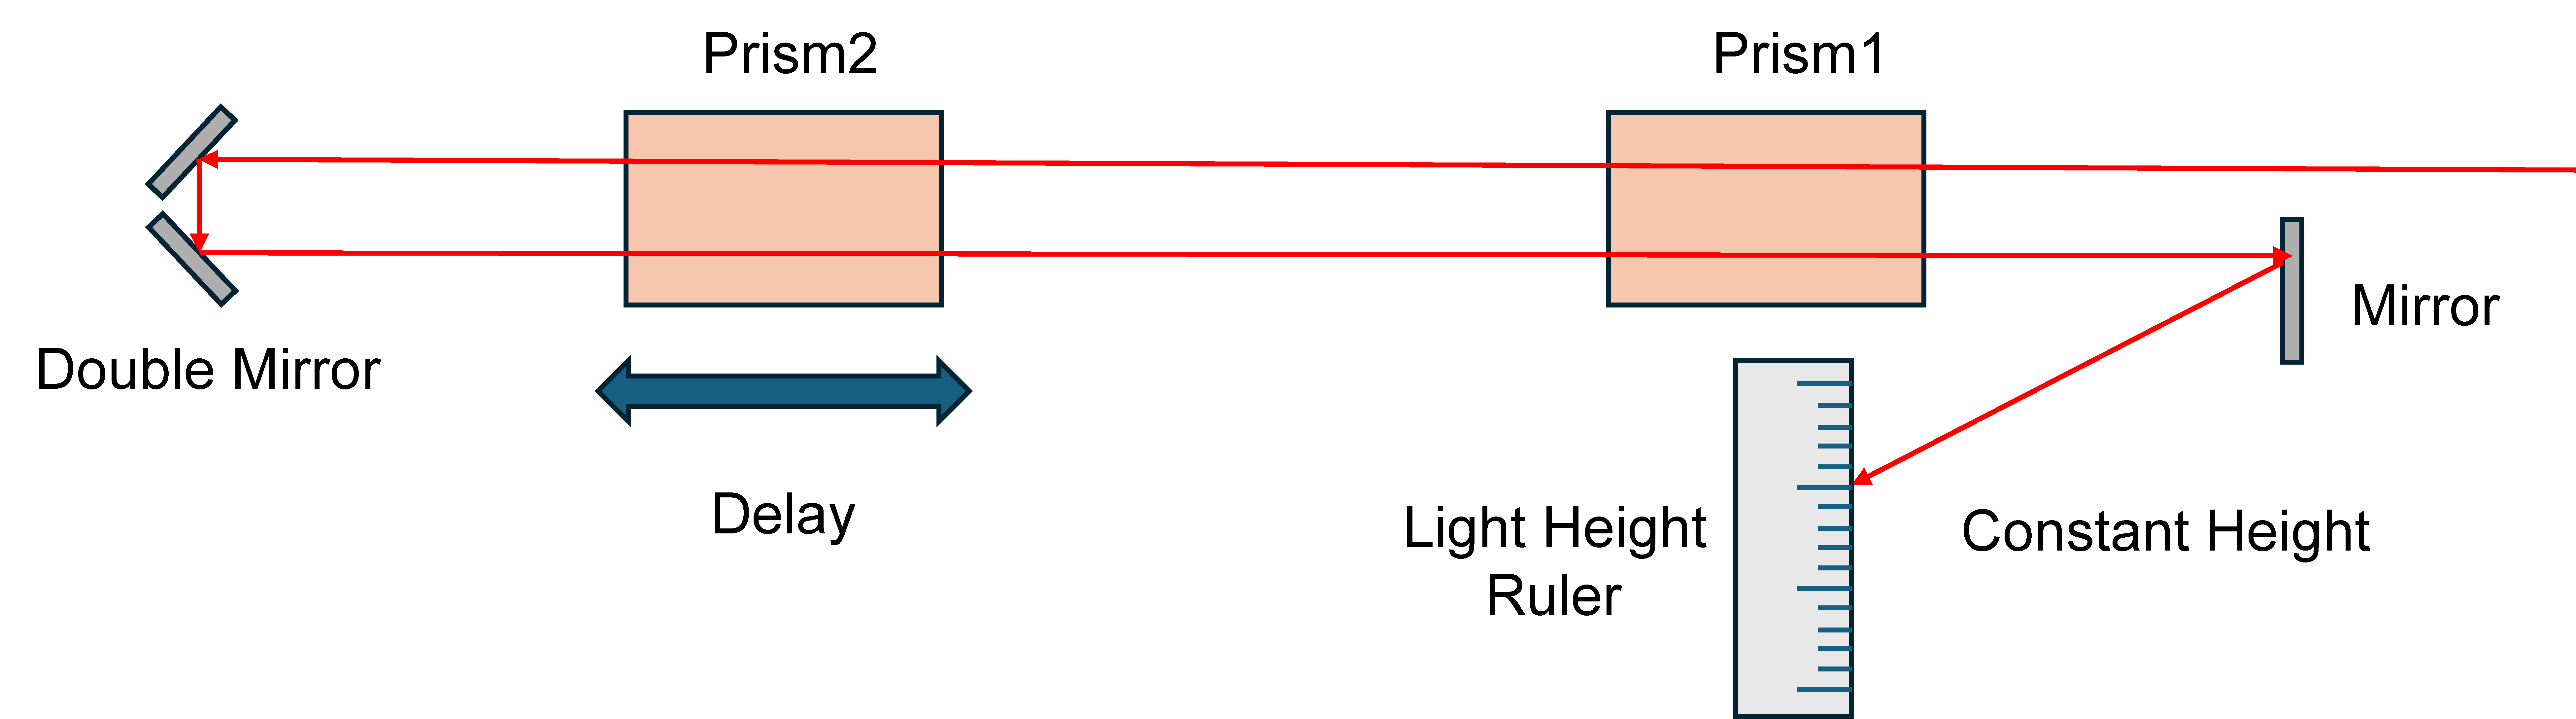
\includegraphics[width=\linewidth]{Fig/FigSup04.pdf}
        \caption{}
        \label{FigSup04}
    \end{subfigure}
    \bicaption{棱镜对压缩器回程结构优化及其对光路稳定性和输出功率的影响。(a) 延迟线调节引起的光路高度变化示意；(b) 调节延迟线引起光路高度变化导致的功率变化；(c) 双反射镜压缩器回程结构优化结果}{Optimization of the prism-pair compressor return path and its influence on optical-path stability and output power. (a) Height variation of the optical path caused by delay-line adjustment; (b) power variation caused by delay-line adjustment; (c) optimized double-mirror return-path design}
    \label{FigSup2-4}
\end{figure}

此外，本文不采用角反射镜(Retroreflector)作为回程器件，主要基于两方面考虑：其一，Retroreflector 通常包含较厚玻璃材料，在近红外波段会引入额外色散和附加吸收，不利于飞秒脉冲压缩；其二，当光路存在轻微偏移时，Retroreflector 内部三次反射同样可能引起光高变化，影响返回光束与系统主光路的重合。因此，从色散控制和输出稳定性两方面看，双反射镜方案更适合本系统的脉冲压缩需求。

棱镜对压缩器的色散补偿主要来源于两部分：一部分来自光束在棱镜材料内部传播所引入的材料色散，通常表现为正色散；另一部分来自不同波长成分在棱镜对之间自由传播时，由于角色散导致的几何色散，通常可提供负色散。通过合理调节棱镜插入深度和两棱镜之间的间距，可以使系统总色散表现为所需的净负色散，从而补偿显微系统后续光路中累积的正色散。

N-SF11 材料的折射率可由 Sellmeier 公式表示为
\begin{equation}
    n^{2}-1=
    \frac{1.7376\lambda^{2}}{\lambda^{2}-0.0132}
    +\frac{0.3137\lambda^{2}}{\lambda^{2}-0.0623}
    +\frac{1.8988\lambda^{2}}{\lambda^{2}-155.2363}
\end{equation}

其中，$\lambda$ 的单位为 $\mathrm{\mu m}$。根据该公式，可进一步求得材料折射率对波长的一阶和二阶导数。在本设计波长附近，计算得到
\begin{align}
    \frac{dn}{d\lambda} &= -0.02085\\
    \frac{d^{2}n}{d\lambda^{2}} &= 0.01446
\end{align}

结合棱镜对色散理论，本文将该压缩器在 920\,nm 附近引入的二阶色散近似表示为
\begin{equation}
    \varphi'' = 0.1285\,x - 0.0052\,L
\end{equation}

其中，$\varphi''$ 表示二阶色散，$x$ 为棱镜插入深度，$L$ 为两块棱镜之间的间距。由该式可见，棱镜插入深度增大时，光束在玻璃中的传播长度增加，材料正色散增大；而增大棱镜间距则会增强由角色散引起的负色散贡献。因此，在压缩器设计中，应尽可能减小棱镜插入深度，以降低附加材料色散，同时通过调节棱镜对间距获得所需的负二阶色散补偿。

从物理机制上看，棱镜对压缩器的调节实质上是在``材料正色散''和``空间负色散''之间寻找平衡。当系统总色散较小时，可通过较浅的插入量和适中的棱镜间距实现补偿；当系统总正色散较大时，则需要适当增加棱镜间距以提供更强的负色散。实验中，棱镜对间距通常结合脉宽测量结果进行优化，即以系统输出端或样品位置处获得最短脉宽为判据，迭代调节压缩器参数，直至获得最佳压缩效果。

需要指出的是，棱镜对压缩器不仅会影响二阶色散，还可能引入一定的三阶色散。对于脉宽较短、光谱较宽的飞秒脉冲而言，高阶色散同样可能对压缩效果产生影响。因此，在实际设计过程中，除了理论计算外，还需要结合自相关仪等脉宽表征手段对压缩效果进行实验验证，以保证补偿后脉冲在显微系统入口处具有较高峰值功率和较好的时间特性。



\subsection{物镜及显微系统总色散的测量与补偿}\label{4.5.3}
\begin{table}[htbp]
\bicaption{等边色散棱镜间距 $L$ 对脉冲压缩效果的影响}{Effect of the equilateral-prism separation $L$ on pulse-compression performance}
\label{Table2}
\centering
\small
\setlength{\tabcolsep}{4pt}
\resizebox{\textwidth}{!}{%
\begin{tabular}{ccccccccccc}
\hline
\rowcolor[HTML]{E7EAED}
\textbf{} &
  \textbf{} &
  \textbf{} &
   &
  \multicolumn{2}{c}{\cellcolor[HTML]{E7EAED}Thorlabs} &
  Newport &
   &
   &
   &
   \\ \hline
\rowcolor[HTML]{E7EAED}
\cellcolor[HTML]{E7EAED} &
  \cellcolor[HTML]{E7EAED} &
  \cellcolor[HTML]{E7EAED} &
  \cellcolor[HTML]{E7EAED} &
  Power 1 &
  Power 2 &
  Power 3 &
  \cellcolor[HTML]{E7EAED} &
  \cellcolor[HTML]{E7EAED} &
  \cellcolor[HTML]{E7EAED} &
  \cellcolor[HTML]{E7EAED} \\
\rowcolor[HTML]{E7EAED}
\multirow{-2}{*}{\cellcolor[HTML]{E7EAED}Session} &
  \multirow{-2}{*}{\cellcolor[HTML]{E7EAED}Group} &
  \multirow{-2}{*}{\cellcolor[HTML]{E7EAED}Position} &
  \multirow{-2}{*}{\cellcolor[HTML]{E7EAED}Laser Power} &
  Laser Out &
  After Compress &
  Into APE &
  \multirow{-2}{*}{\cellcolor[HTML]{E7EAED}Type} &
  \multirow{-2}{*}{\cellcolor[HTML]{E7EAED}PMT Seneor} &
  \multirow{-2}{*}{\cellcolor[HTML]{E7EAED}Gain} &
  \multirow{-2}{*}{\cellcolor[HTML]{E7EAED}Sech2 Width} \\ \hline
\rowcolor[HTML]{E7EAED}
\cellcolor[HTML]{E7EAED} &
  1 &
  \cellcolor[HTML]{FFC000}250cm &
  50\% &
  0.493 W &
  0.198 W &
  17.05 mW &
  Autocorrelator &
  Sensor 2 &
  530 &
  145 $\pm$ 8fs \\
\rowcolor[HTML]{E7EAED}
\cellcolor[HTML]{E7EAED} &
  2 &
  \cellcolor[HTML]{FFC000}250cm &
  100\% &
  0.828 W &
  0.362 W &
  19.33 mW &
  Autocorrelator &
  Sensor 2 &
  500 &
  147 $\pm$ 5fs \\
\rowcolor[HTML]{E7EAED}
\multirow{-3}{*}{\cellcolor[HTML]{E7EAED}1} &
  3 &
  \cellcolor[HTML]{FFC000}250cm &
  100\% &
  0.828 W &
  0.362 W &
  19.33 mW &
  Autocorrelator &
  Sensor 1 &
  600 &
  146 $\pm$ 10fs \\ \hline
\rowcolor[HTML]{E7EAED}
\cellcolor[HTML]{E7EAED} &
  1 &
  \cellcolor[HTML]{83CBEB}350cm &
  50\% &
  0.497 W &
  0.208 W &
  15.14 mW &
  Autocorrelator &
  Sensor 2 &
  550 &
  138 $\pm$ 5fs \\
\rowcolor[HTML]{E7EAED}
\cellcolor[HTML]{E7EAED} &
  2 &
  \cellcolor[HTML]{83CBEB}350cm &
  100\% &
  0.825 W &
  0.379 W &
  20.43 mW &
  Autocorrelator &
  Sensor 1 &
  640 &
  140 $\pm$ 10fs \\
\rowcolor[HTML]{E7EAED}
\multirow{-3}{*}{\cellcolor[HTML]{E7EAED}2} &
  3 &
  \cellcolor[HTML]{83CBEB}350cm &
  100\% &
  0.825 W &
  0.379 W &
  20.43 mW &
  Autocorrelator &
  Sensor 2 &
  520 &
  135 $\pm$ 3fs \\ \hline
\rowcolor[HTML]{E7EAED}
\cellcolor[HTML]{E7EAED} &
  1 &
  \cellcolor[HTML]{E59EDD}450cm &
  100\% &
  0.867 W &
  0.373 W &
  19.58 mW &
  Autocorrelator &
  Sensor 2 &
  550 &
  133 $\pm$ 5fs \\
\rowcolor[HTML]{E7EAED}
\multirow{-2}{*}{\cellcolor[HTML]{E7EAED}3} &
  2 &
  \cellcolor[HTML]{E59EDD}450cm &
  100\% &
  0.867 W &
  0.373 W &
  19.58 mW &
  Autocorrelator &
  Sensor 1 &
  630 &
  135 $\pm$ 10fs \\ \hline
\rowcolor[HTML]{E7EAED}
\cellcolor[HTML]{E7EAED} &
  1 &
  \cellcolor[HTML]{8ED973}550cm &
  100\% &
  0.869W &
  0.362 W &
  13.73 mW &
  Autocorrelator &
  Sensor 2 &
  540 &
  135 $\pm$ 5fs \\
\rowcolor[HTML]{E7EAED}
\multirow{-2}{*}{\cellcolor[HTML]{E7EAED}4} &
  2 &
  \cellcolor[HTML]{8ED973}550cm &
  100\% &
  0.869W &
  0.362 W &
  13.73 mW &
  Autocorrelator &
  Sensor 1 &
  670 &
  130 $\pm$ 20fs \\ \hline
\end{tabular}%
}
\vspace{2mm}
\begin{minipage}{\textwidth}
\footnotesize
\textit{注：实验中关闭了 920\,nm 激光器内部的体光栅补偿装置，脉宽测量仪器为 APE PulseCheck NX 自相干仪。}
\end{minipage}
\end{table}

在棱镜对压缩器完成初步设计后，还需要进一步考虑显微系统中所有后续光学元件引入的总色散，包括扫描光学、中继透镜、分光元件以及物镜本身带来的附加色散。对于高数值孔径多光子显微镜而言，物镜通常是系统中引入色散最显著的元件之一，因此单纯在显微镜入口处完成预压缩并不足以保证样品处获得最短脉宽，还需要结合物镜后的实际脉宽测量结果对压缩器进行进一步优化。

在本文工作中，一方面利用 Zemax 对显微系统中主要光学元件的传播路径和材料组成进行建模分析，以估算系统的总群延迟色散；另一方面在实验上通过自相关仪直接测量补偿前后脉冲在系统末端的时间展宽情况，从而实现理论计算与实验调节的结合。该方法能够更准确地反映实际系统中材料色散、光路长度变化以及装调误差共同作用下的总色散情况。

如表~\ref{Table2} 所示，本文通过调节等边色散棱镜之间的相对距离 $L$，记录激光经过补偿后的脉冲宽度变化。共测试了四组棱镜间距，每组重复 2--3 次。结果表明，当两棱镜的相对距离约为 450\,cm 左右时，系统对 920\,nm 激光输出具有较好的压缩效果，可将脉宽稳定压缩到约 130--135\,fs 的范围内。若系统后续继续加入其他光学元件导致总色散增加，则仍可通过对棱镜间距进行微调来实现进一步补偿。

\begin{figure}[htbp]
    \centering
    \begin{subfigure}{0.45\linewidth}
        \centering
        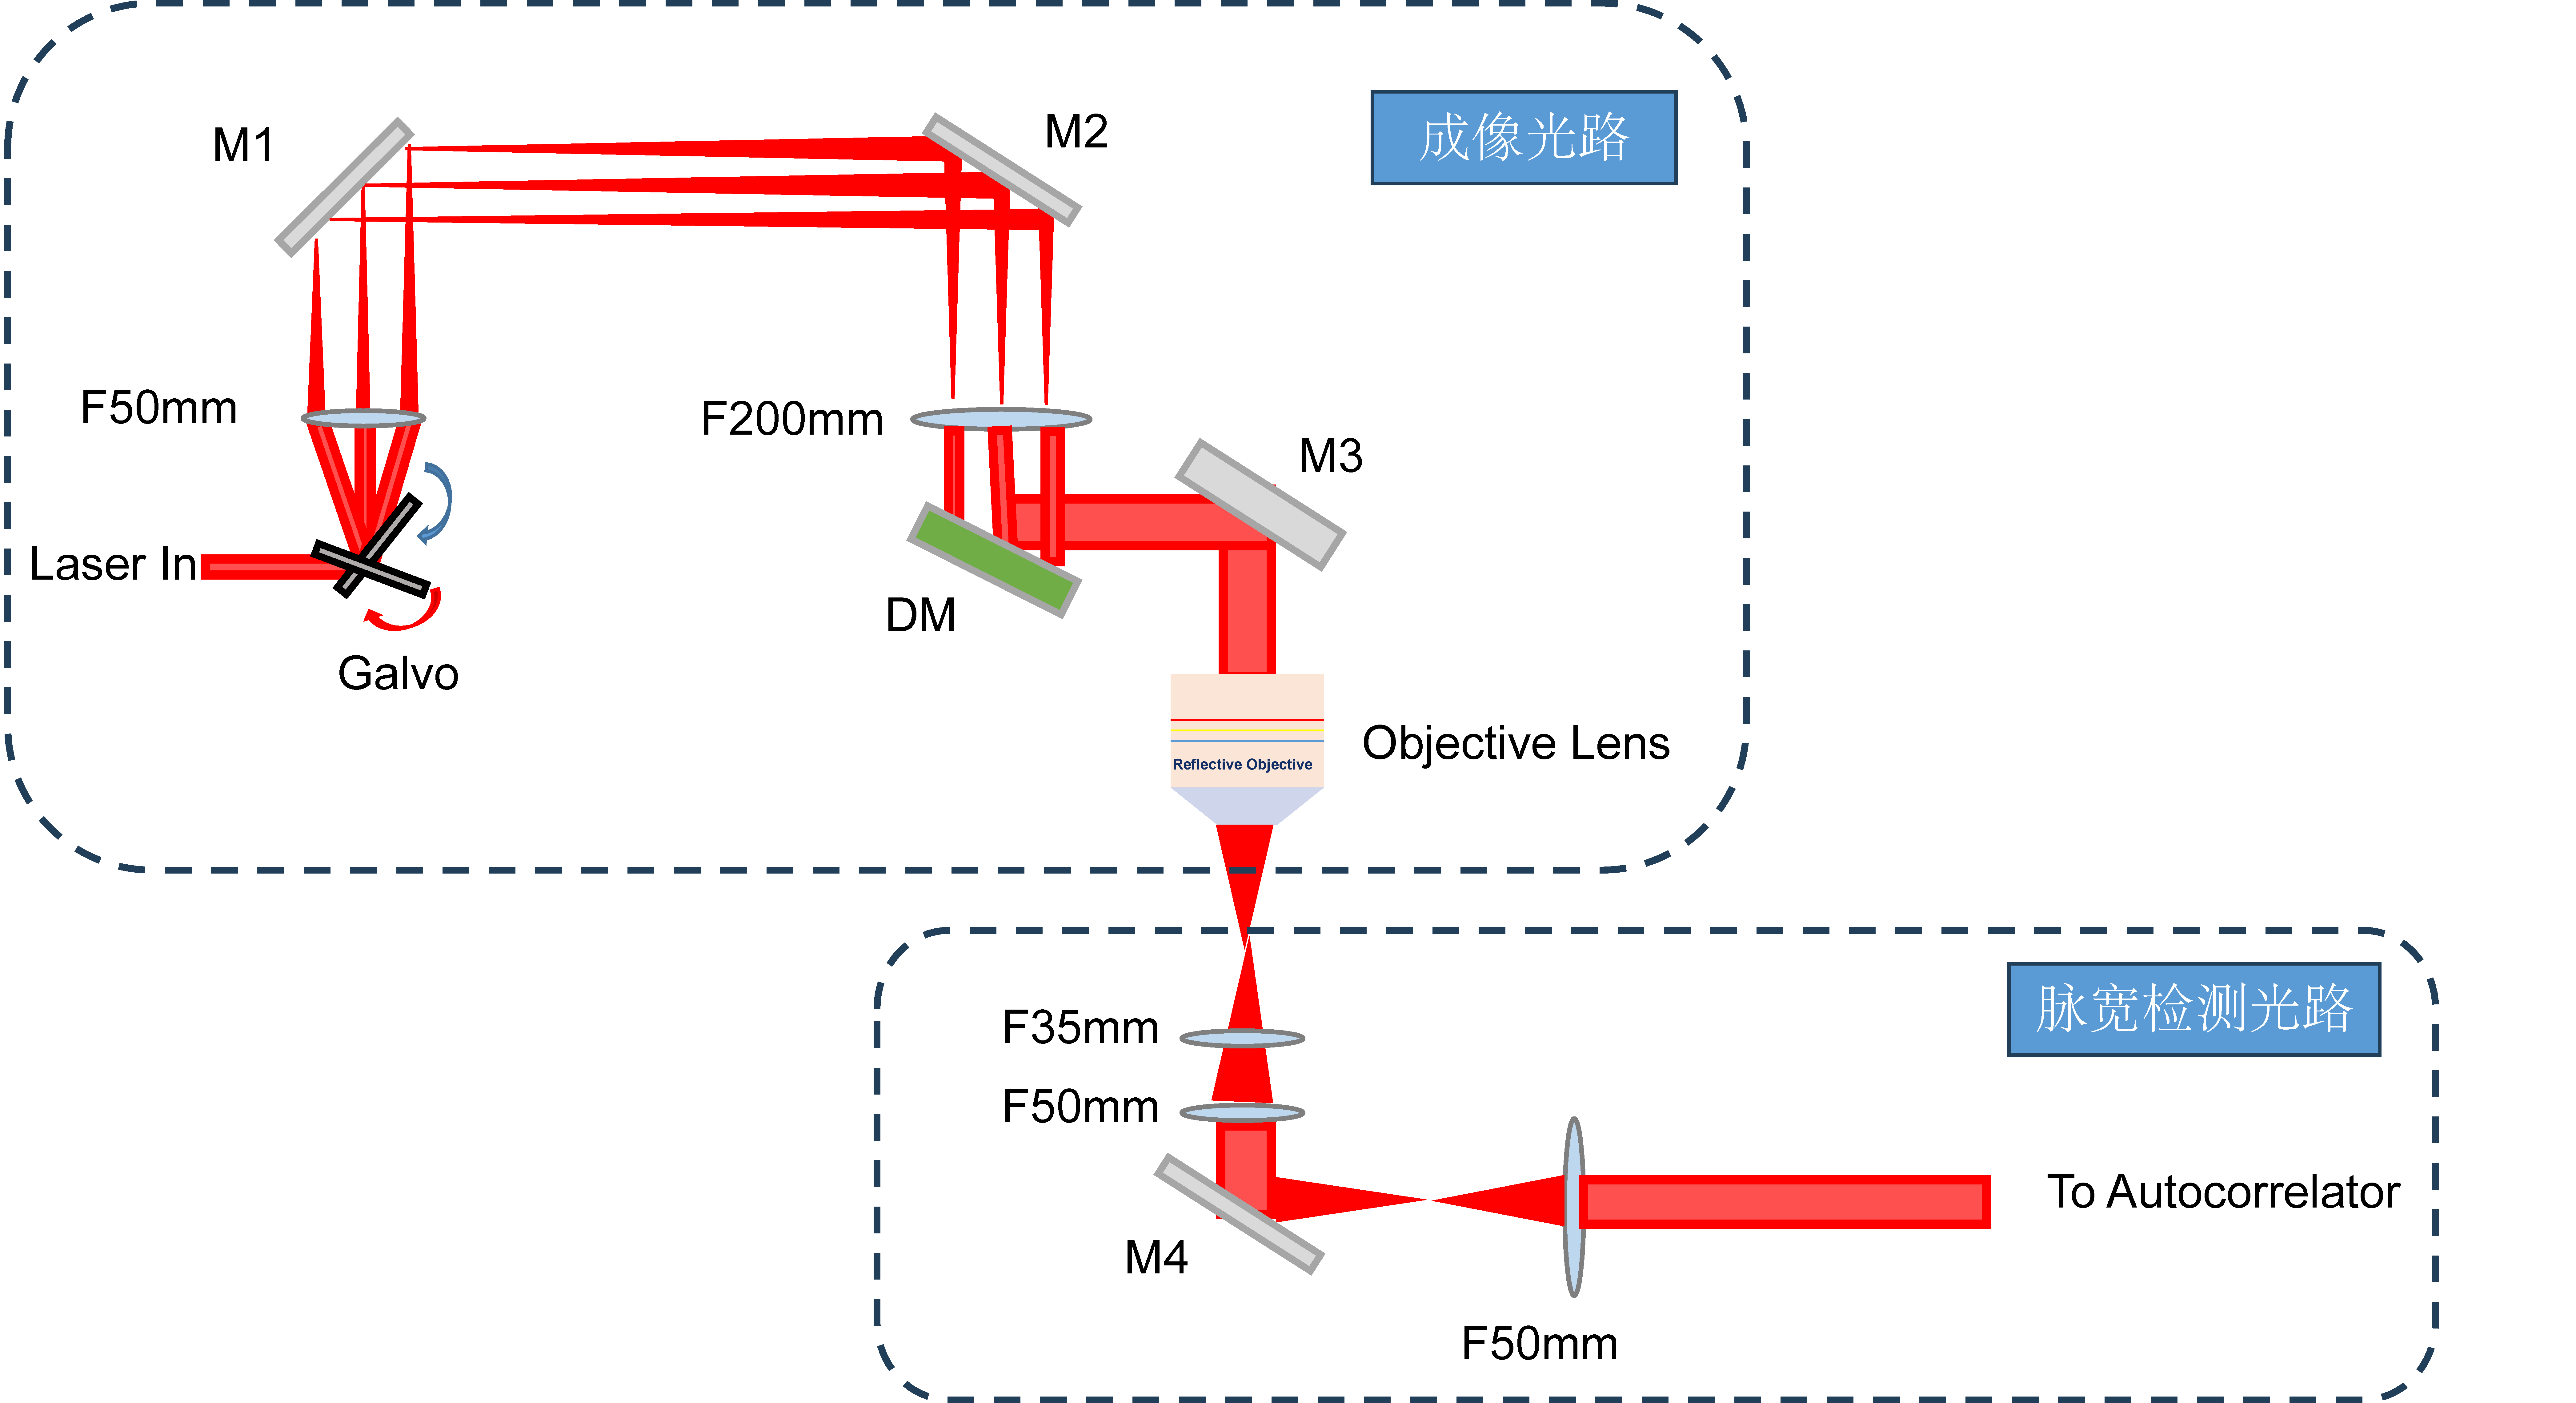
\includegraphics[width=\linewidth]{Fig/Fig13.pdf}
        \caption{}
        \label{Fig13}
    \end{subfigure}%
    \hspace{0.03\linewidth}%
    \begin{subfigure}{0.45\linewidth}
        \centering
        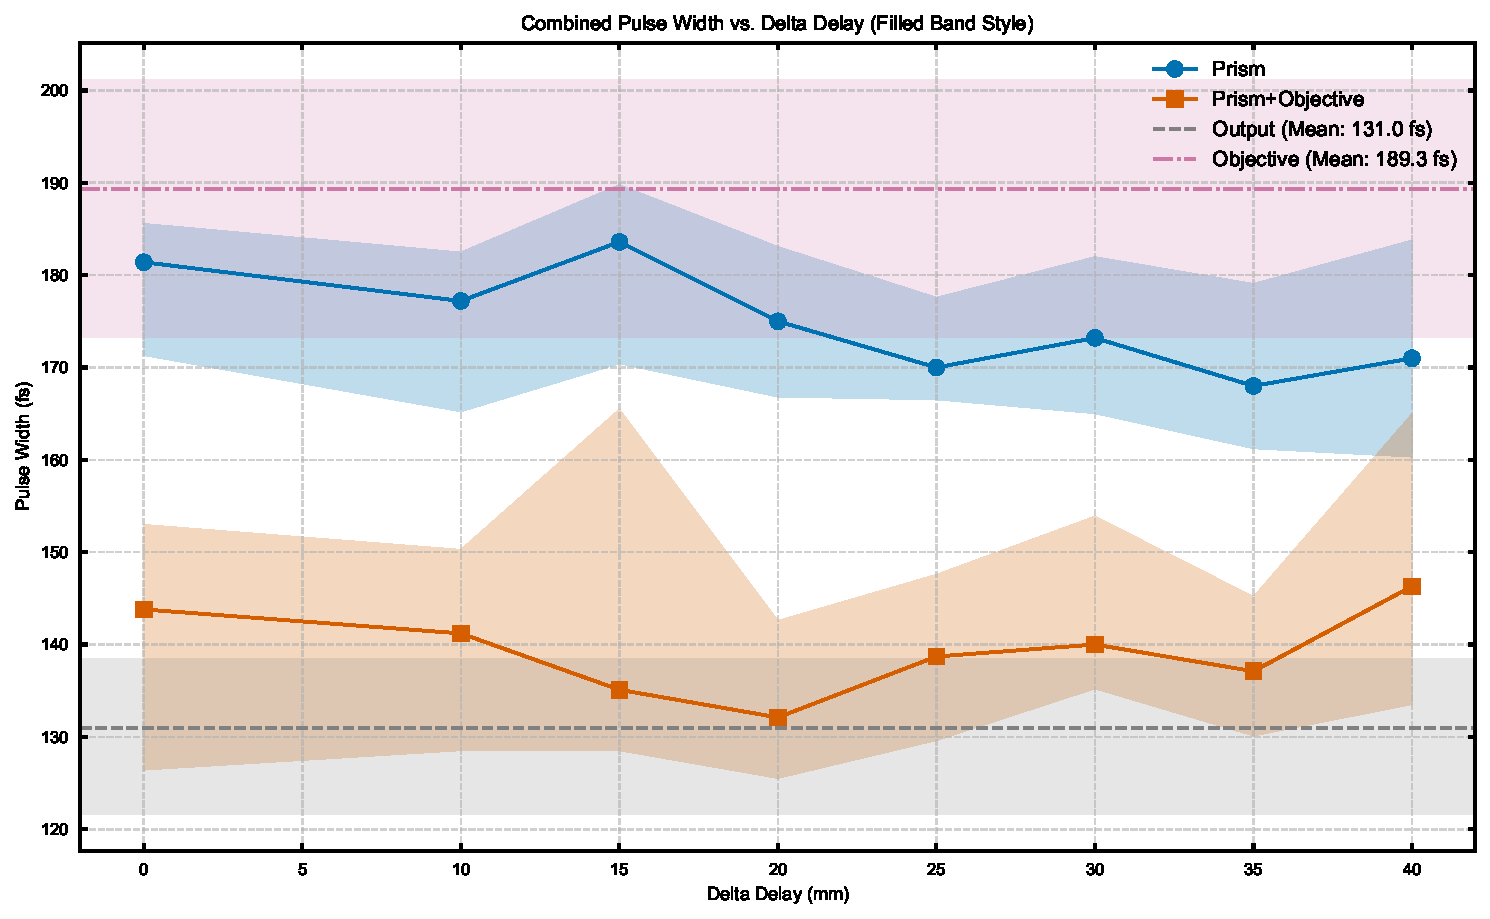
\includegraphics[width=\linewidth]{Fig/Fig14.pdf}
        \caption{}
        \label{Fig14}
    \end{subfigure}
    \bicaption{显微系统总色散补偿方案及物镜后脉宽测量。(a) 系统末端脉宽测量光路；(b) 补偿前后脉宽对比结果}{Overall dispersion-compensation scheme of the microscope system and pulse-width measurement after the objective. (a) Optical layout for pulse-width measurement at the system output; (b) comparison of pulse widths before and after compensation}
    \label{fig13-14}
\end{figure}

图~\ref{fig13-14} 给出了对显微镜所有光学元件总色散进行统一补偿的实验方案。通过在物镜后放置小焦距透镜，将光束聚焦到自相关仪上测量其脉冲宽度，并通过微调色散补偿棱镜对系统总色散进行补偿。实验结果表明，未补偿时，经过物镜及系统其他光学元件后的脉宽约为 189.3\,fs；在优化棱镜参数后，物镜后输出脉宽可压缩至约 131\,fs。该结果说明，棱镜对压缩器不仅能够有效补偿扫描系统和中继光学引入的色散，还能够显著减小物镜带来的附加脉冲展宽，从而提高样品处的多光子激发效率。





\subsection{基于双光子吸收的自相干脉宽表征与实验验证}\label{4.5.4}

为验证棱镜对补偿后显微系统末端脉宽的变化，本文在第四章主线中保留了自相干仪的结构设计、实验对比与误差分析。有关平均功率与脉冲稳定性标定、干涉自相关的数学模型、去相关因子以及啁啾识别等更偏方法学的补充内容，则统一整理至附录。

为实现对超快激光脉冲宽度的准确表征，本文设计并搭建了一套基于迈克尔逊干涉仪结构的自相干测试系统。该系统以光电二极管作为非线性探测元件，相较于传统``非线性晶体 $+$  光电倍增管 $+$  滤光片''的方案，具有结构更紧凑、调试更简便、成本更低等优点。

其基本工作过程如下：待测红外飞秒脉冲入射至迈克尔逊干涉仪后，经分光平片分为两束振幅近似相等的光束。其中一路经固定臂反射返回，另一路经由高精度位移台控制的移动臂反射返回。通过调节移动臂位移 $\Delta x$，可在两束光之间引入可控的时间延迟

\begin{equation}\label{tau}
\tau = \frac{2\Delta x}{c}
\end{equation}

其中 $c$ 为真空中的光速。随后两束光重新合束，并被共同聚焦到光电二极管表面，在探测器中通过双光子吸收过程产生与时间延迟相关的非线性响应信号。

\begin{figure}[htbp]
    \centering
    \begin{subfigure}[b]{0.39\linewidth}
        \centering
        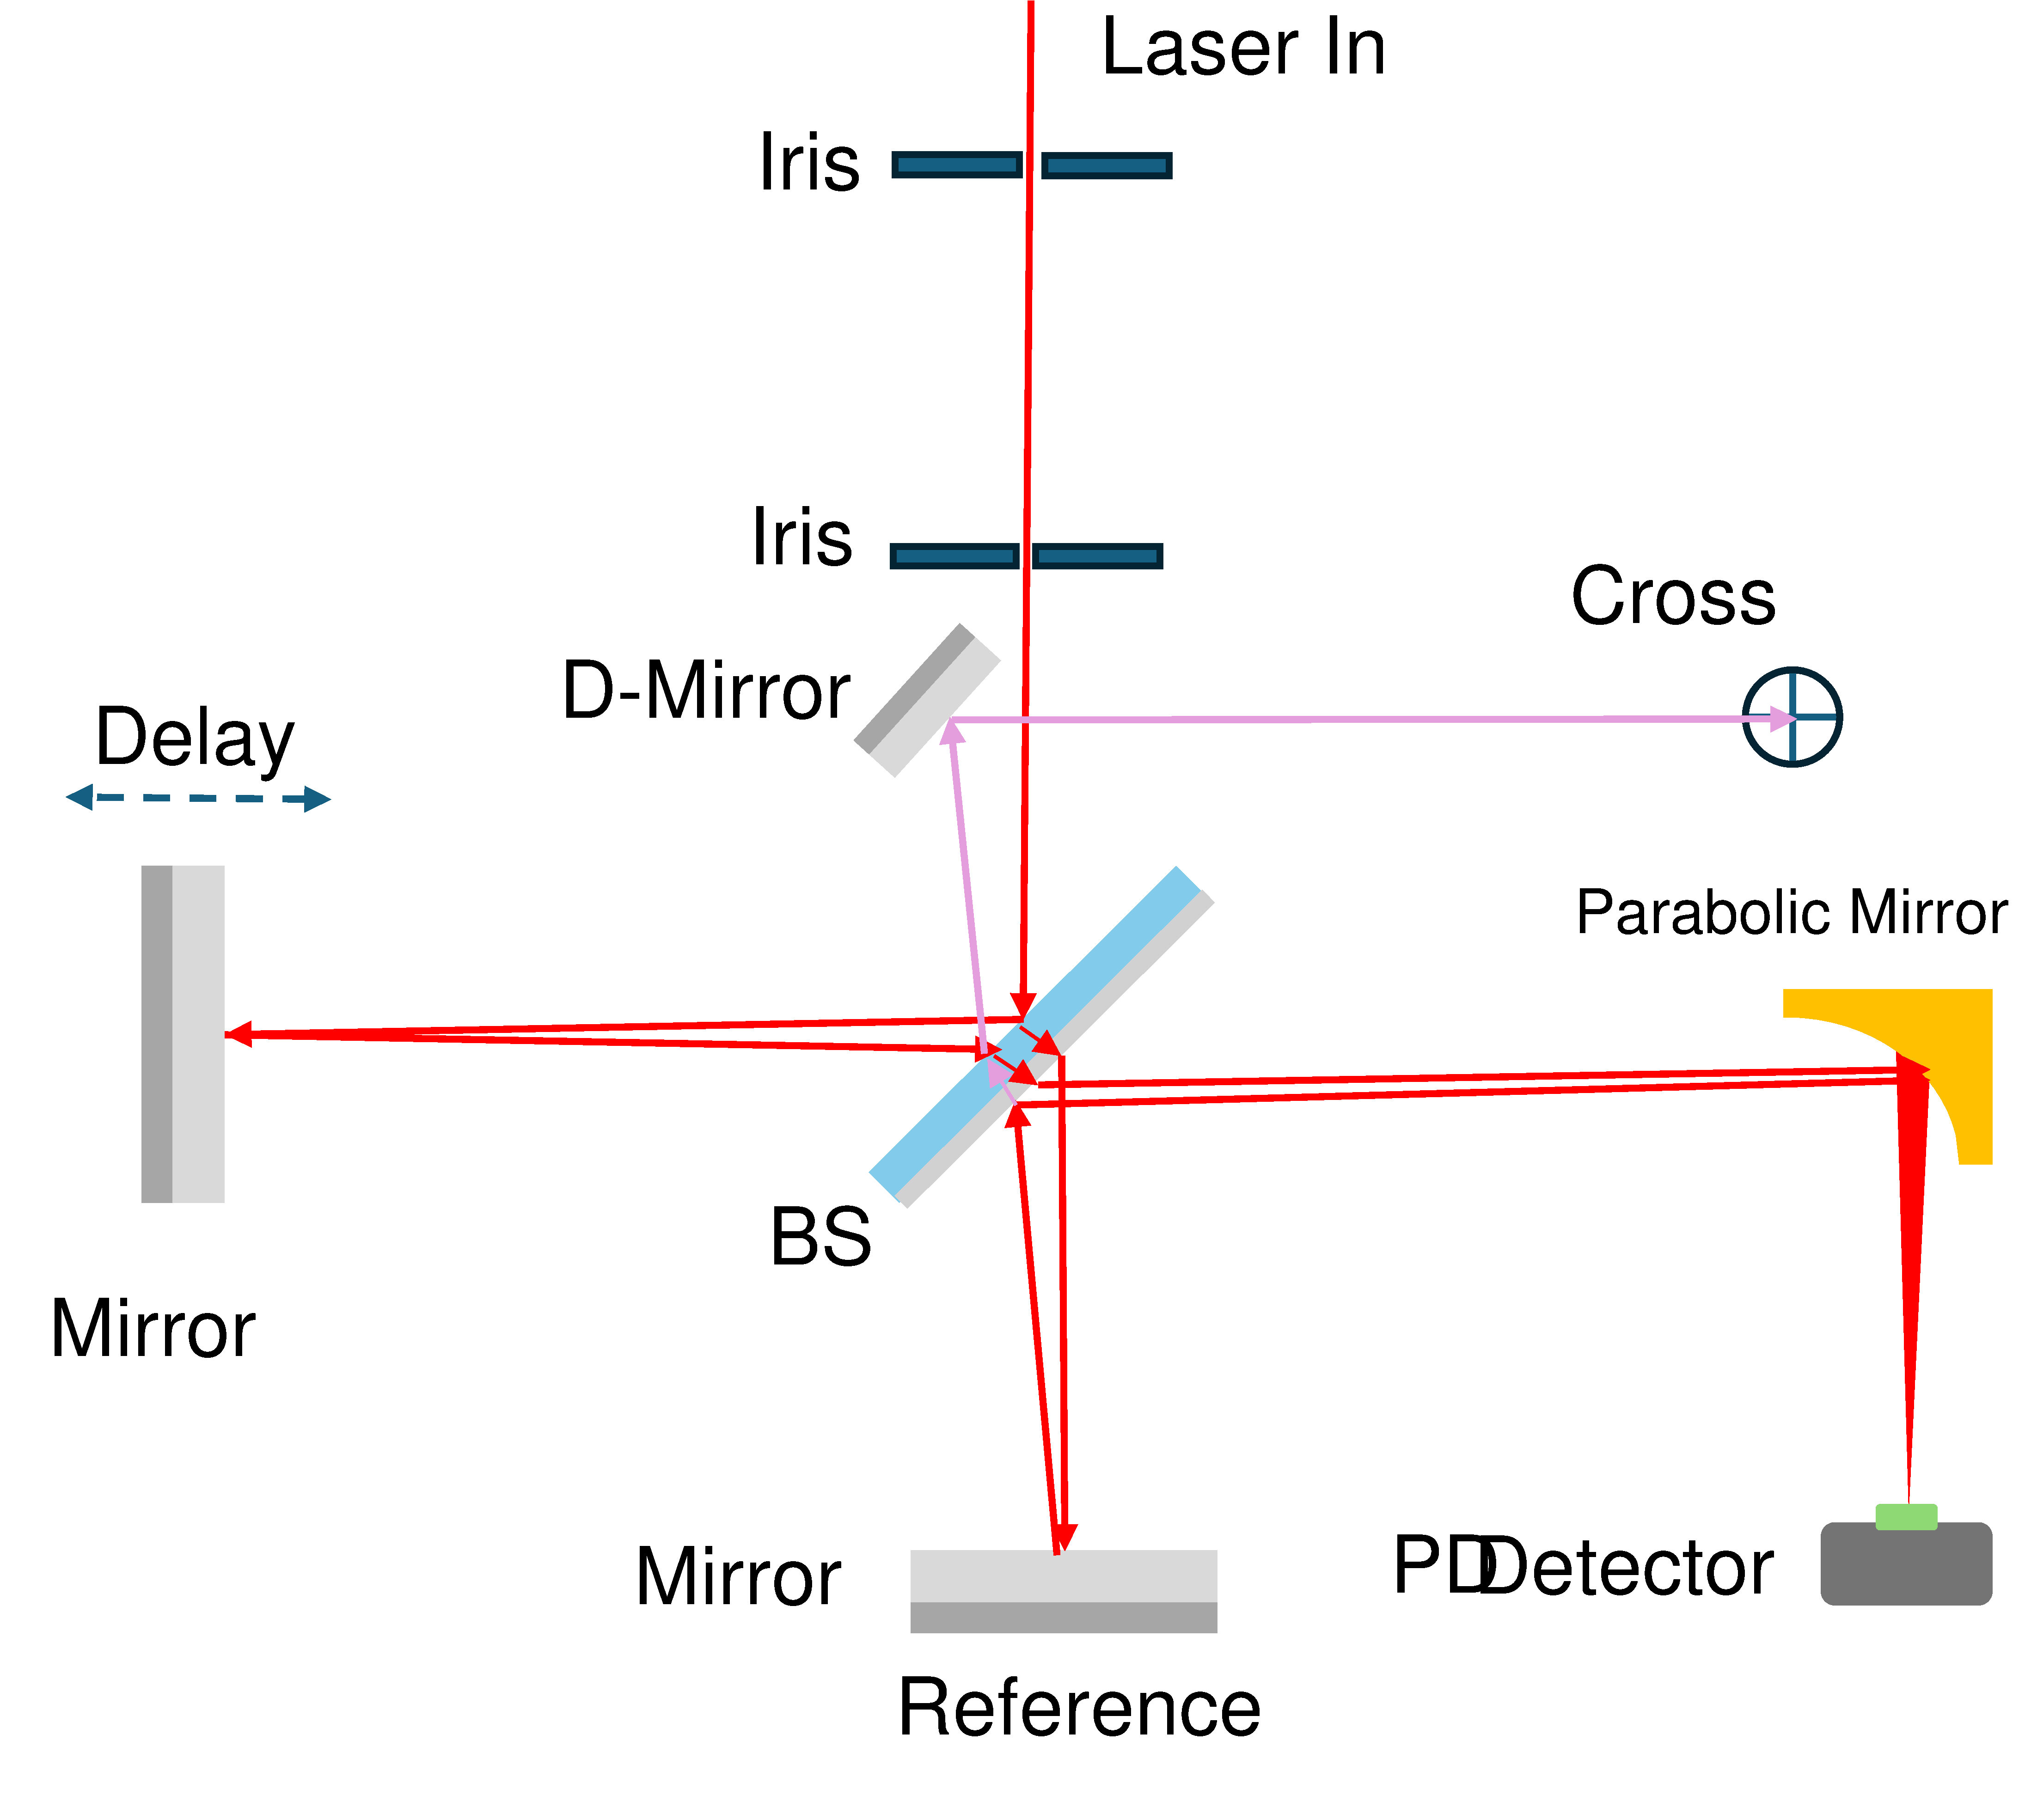
\includegraphics[width=\linewidth]{Fig/Fig39.1-1.pdf}
        \caption{}
        \label{fig39.1-1}
    \end{subfigure}
    \hfil
    \begin{subfigure}[b]{0.45\linewidth}
        \centering
        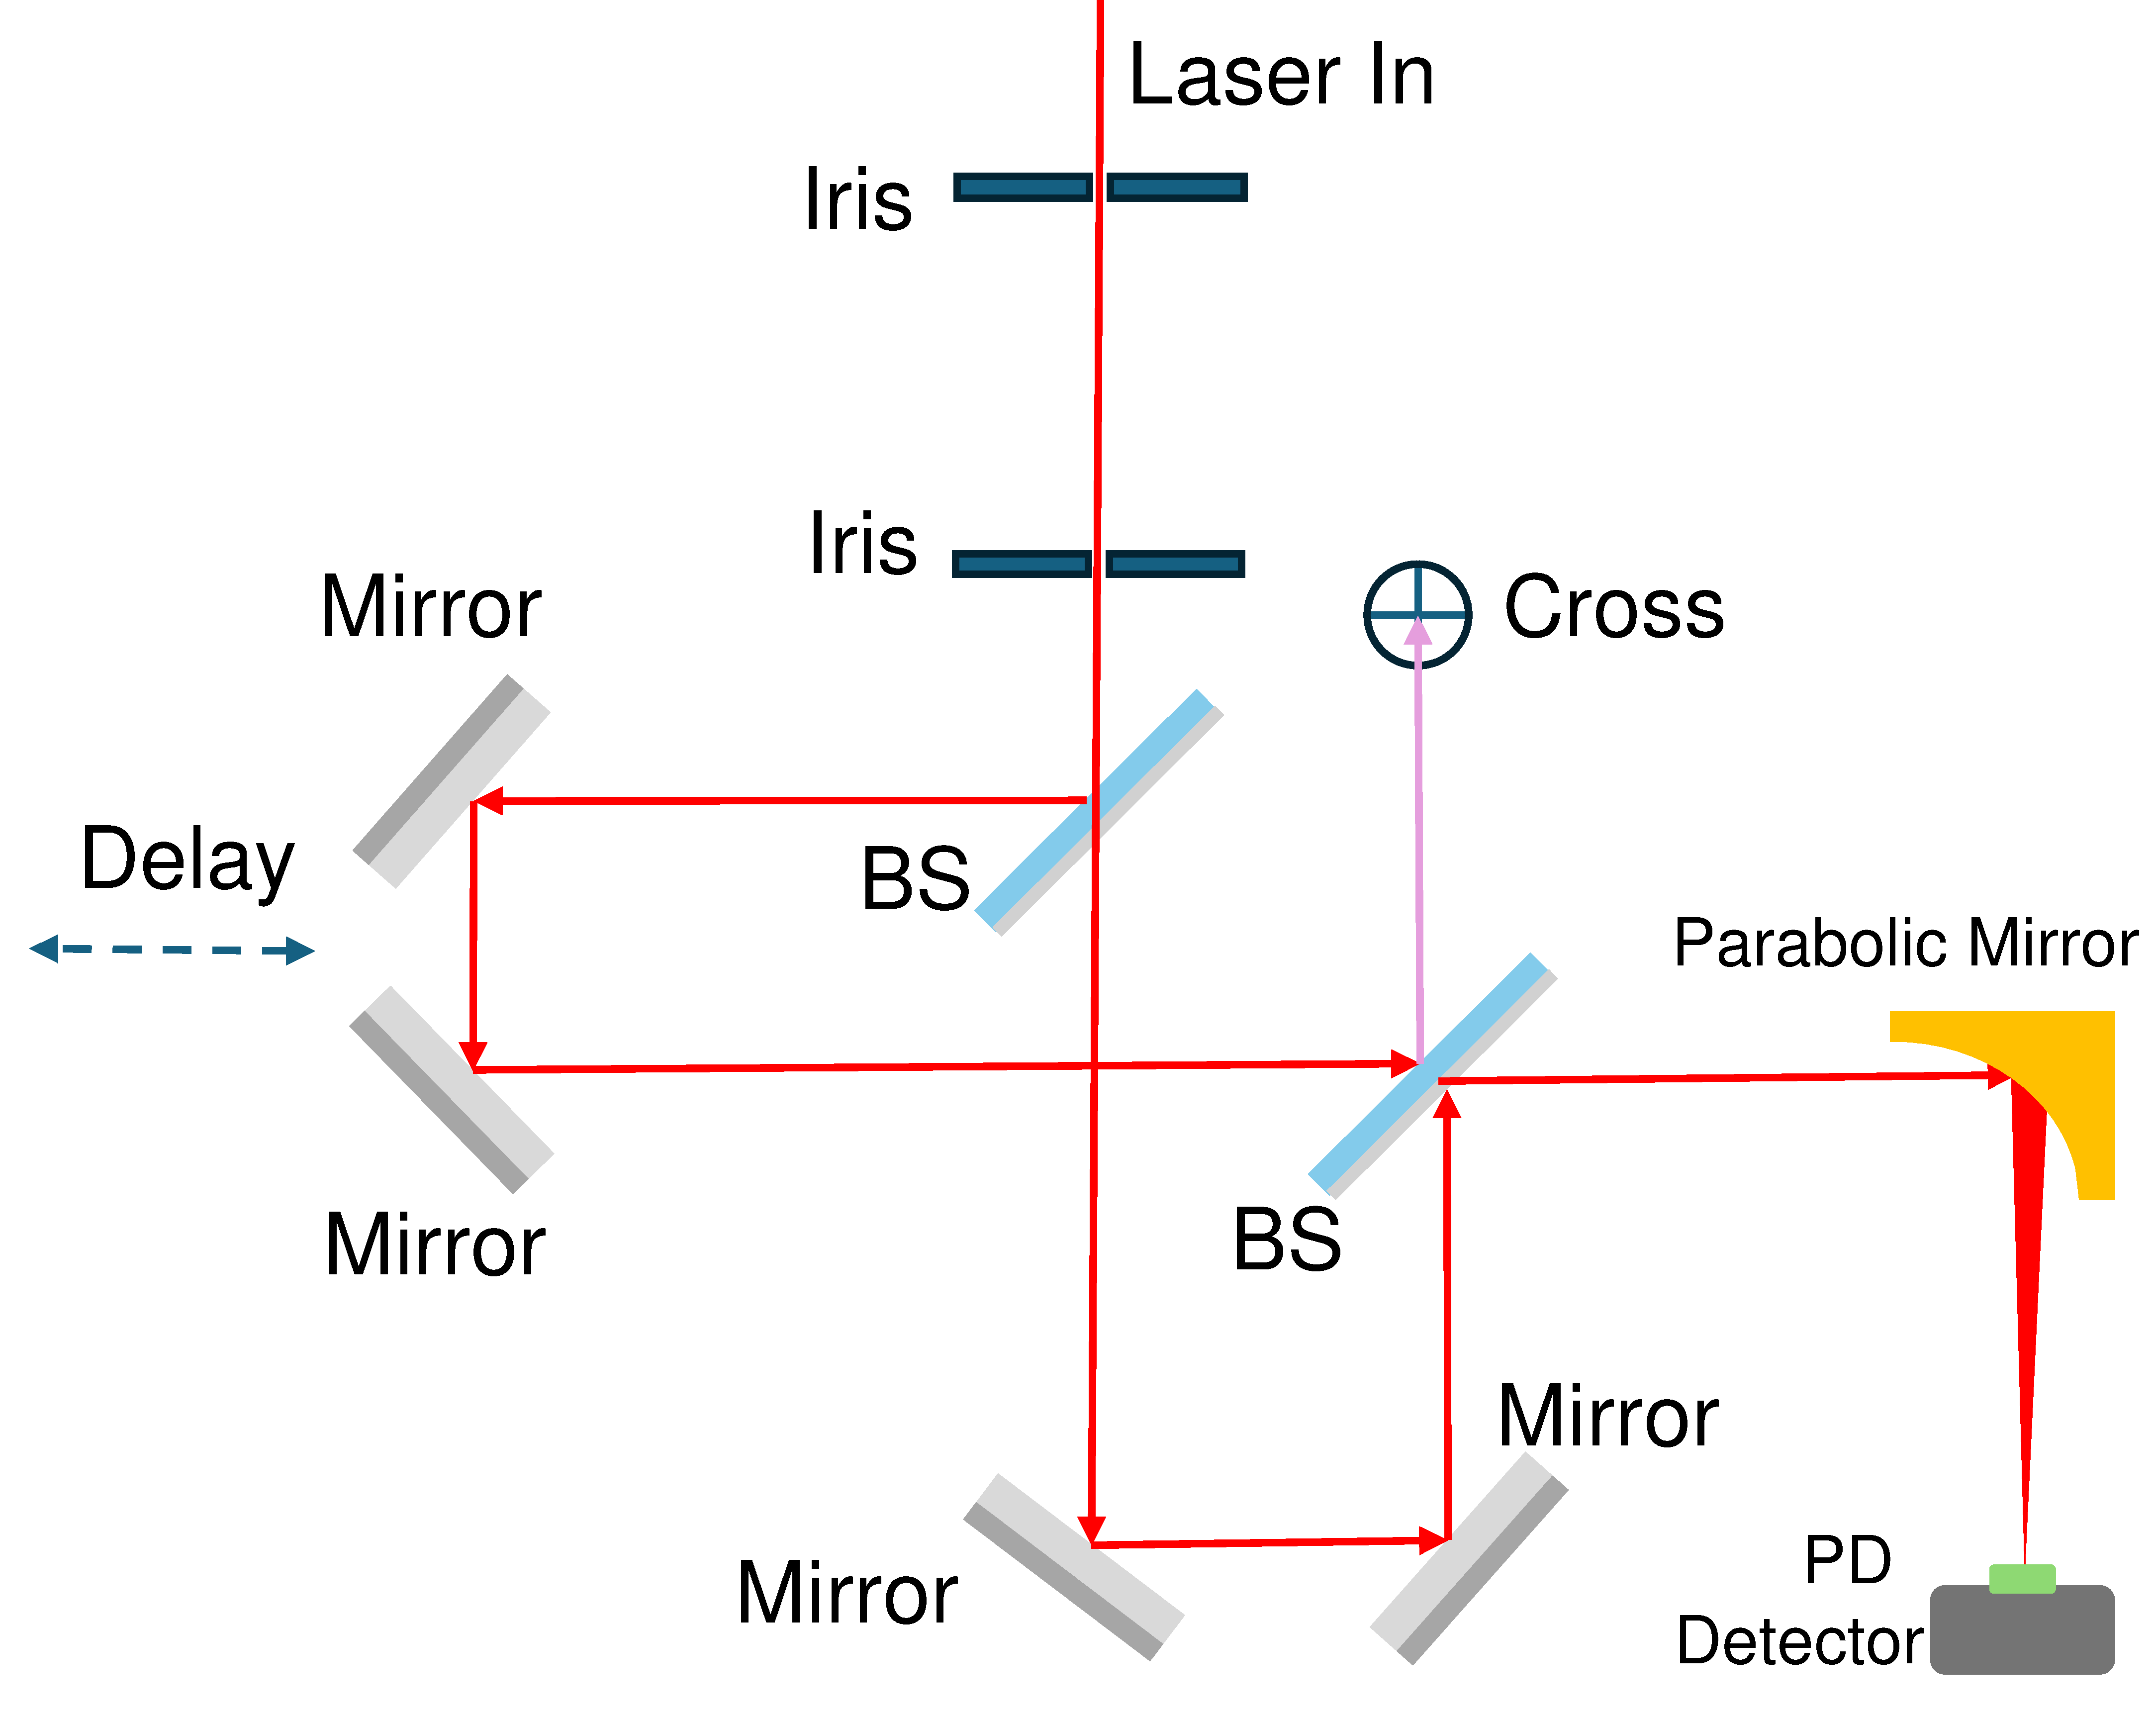
\includegraphics[width=\linewidth]{Fig/Fig39.1-2.pdf}
        \caption{}
        \label{fig39.1-2}
    \end{subfigure}
    \bicaption{基于迈克尔逊干涉原理设计的两版自相干仪光路结构。(a) 第一版自相干仪，单分光片结构；(b) 第二版自相干仪，双分光片结构}{Optical layouts of two autocorrelator designs based on the Michelson interferometer principle. (a) First-generation autocorrelator with a single beam splitter; (b) second-generation autocorrelator with a dual-beam-splitter configuration}
    \label{fig39.1}
\end{figure}

如图~\ref{fig39.1} 所示，本文先后设计并搭建了两版自相干仪。图~\ref{fig39.1}(\subref{fig39.1-1}) 所示为第一版方案，其基本结构采用常规迈克尔逊干涉仪。为了便于观察两束回光的重合情况，该方案通过对其中一路反射镜施加微小倾角，使参考光在空间上形成可辨识的偏移，并借助十字叉丝辅助完成光路校准。该方案能够实现基础的干涉测量，但由于两束光在聚焦位置存在一定交叉角，难以在探测面上实现严格共线重合，从而会降低干涉对比度；同时，反射镜倾斜还可能引入额外的偏振态变化，进一步影响相干叠加效果。

为解决上述问题，本文进一步设计了第二版自相干仪，如图~\ref{fig39.1}(\subref{fig39.1-2}) 所示。该方案采用双分光平片结构，使两束光在整个传播过程中均保持标准反射几何关系，从而避免了因镜面倾斜带来的空间夹角和偏振扰动。与第一版相比，第二版方案能够更好地保证两束光在合束后的空间共线性与偏振一致性，因此可获得更高的干涉对比度和更稳定的自相关信号。这一改进对提升系统测量精度和重复性具有重要意义。

\begin{figure}[htbp]
    \centering
    \begin{subfigure}[b]{0.45\textwidth}
        \centering
        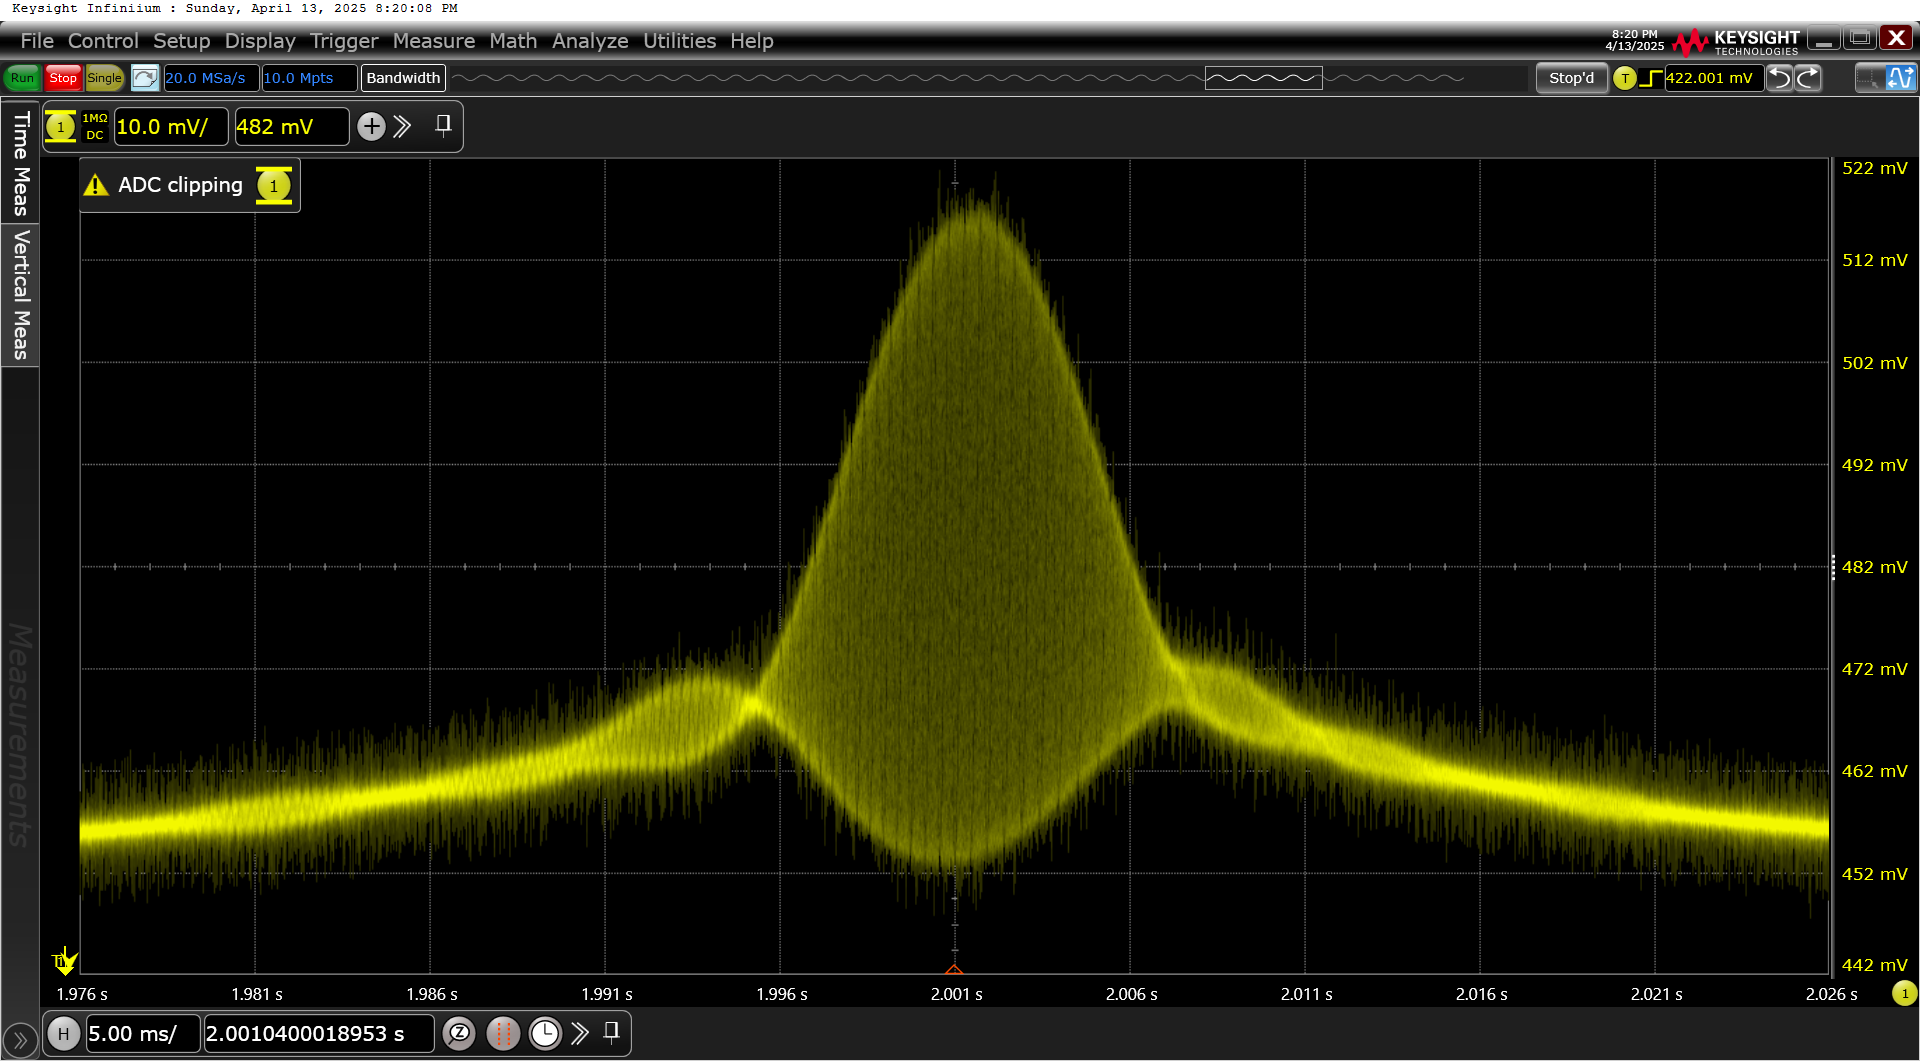
\includegraphics[width=\textwidth]{Fig/Fig39.png}
        \caption{}
        \label{fig39}
    \end{subfigure}
    \begin{subfigure}[b]{0.45\textwidth}
        \centering
        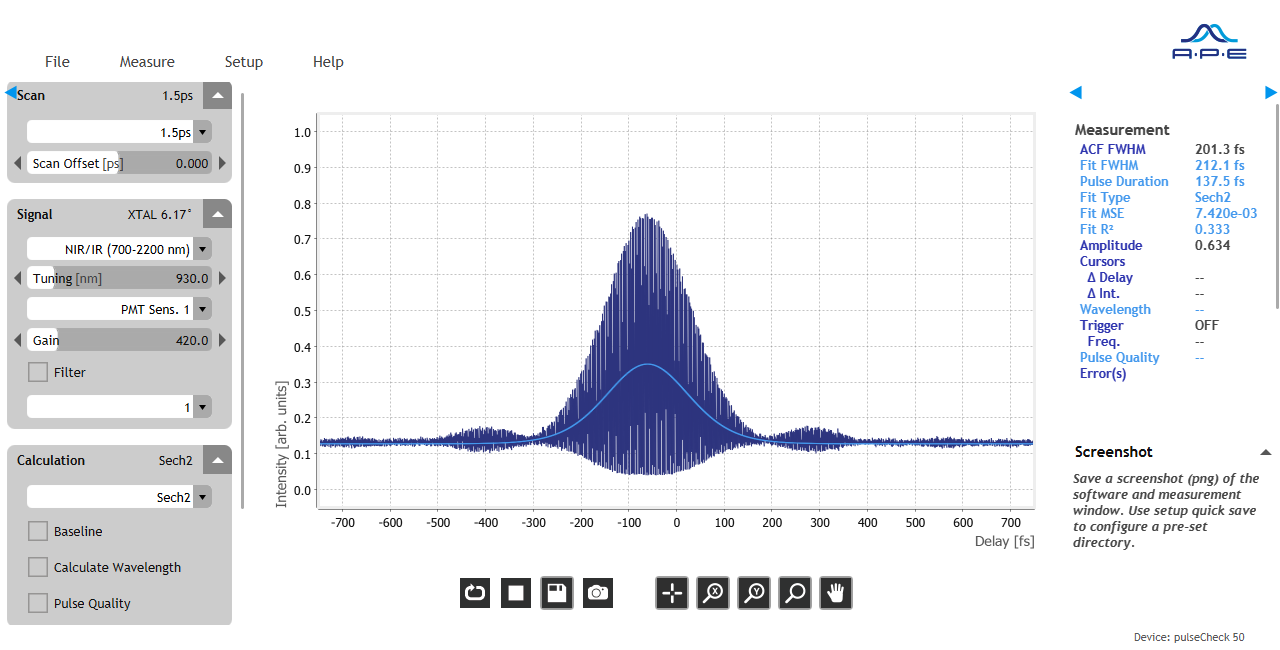
\includegraphics[width=\textwidth]{Fig/Fig40.png}
        \caption{}
        \label{fig40}
    \end{subfigure}
    \bicaption{DIY 自相干仪与商用自相干仪测量结果对比。(a) DIY 自相干仪测得的干涉自相关曲线；(b) APE PulseCheck NX 测得的脉冲宽度结果}{Comparison between measurements from the DIY autocorrelator and a commercial autocorrelator. (a) Interferometric autocorrelation trace measured with the DIY setup; (b) pulse-width result measured with the APE PulseCheck NX}
    \label{fig39-40}
\end{figure}

在探测器的选择上，本文选用了对紫外至可见波段具有较高响应灵敏度的宽禁带半导体探测器。例如，磷镓(GaP) 探测器的典型响应范围约为 $150~\mathrm{nm}\sim550~\mathrm{nm}$，磷砷化镓(GaAsP) 探测器的响应范围约为 $300~\mathrm{nm}\sim680~\mathrm{nm}$。对于波长约为 $1030~\mathrm{nm}$ 的红外基频飞秒脉冲，其单光子能量低于探测器材料的禁带宽度，因此探测器对该基频光几乎不产生线性响应，这使得系统能够在硬件层面天然抑制基频红外信号的直接干扰。

然而，当两束飞秒脉冲在探测器表面于时间上充分重合时，其瞬时峰值功率显著提高，可在半导体材料内部诱导双光子吸收过程，并产生与二次谐波等效波长对应的光生电流信号。通过记录该非线性光电流随时间延迟变化的曲线，并结合脉冲包络模型及去相关因子，即可反演得到待测脉冲的实际宽度。

\begin{figure}[htbp]
    \centering
    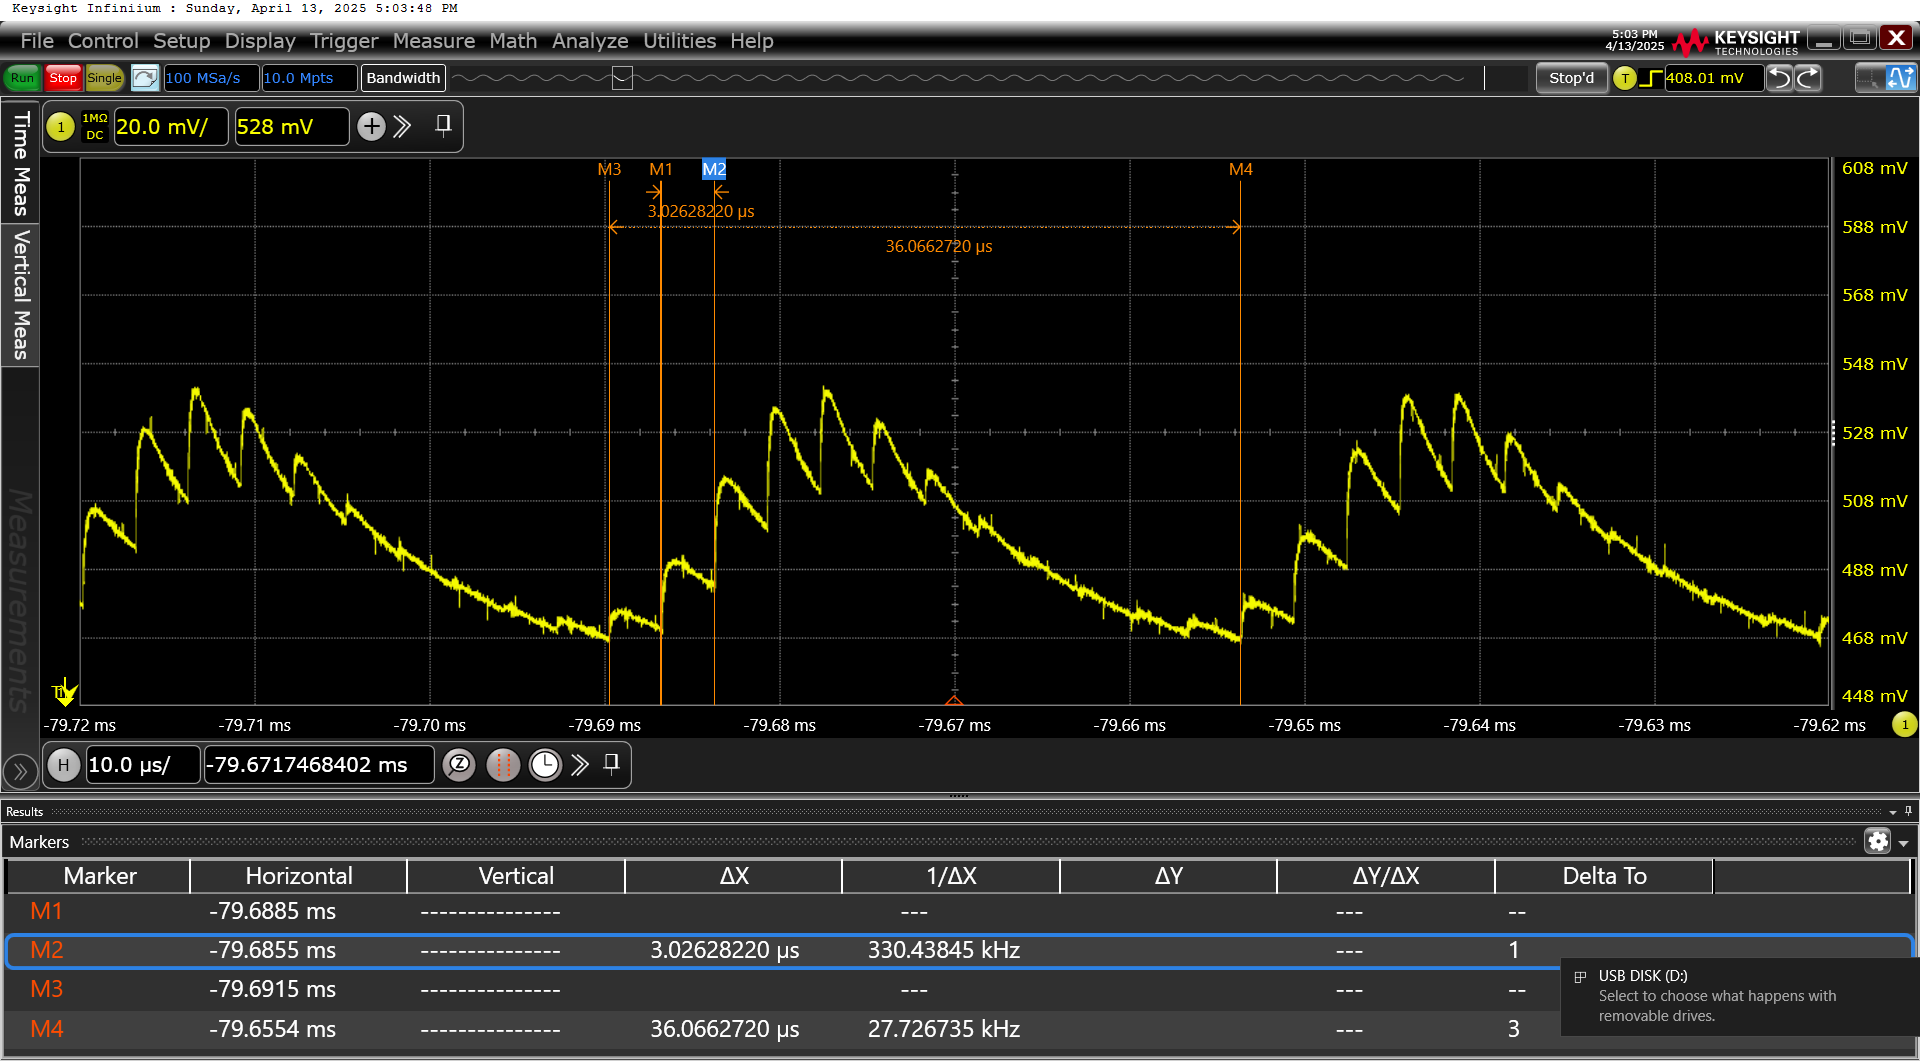
\includegraphics[width=0.75\textwidth]{Fig/Fig43.png}
    \bicaption{放大后的自相干包络中出现的基频干扰信号}{Fundamental-frequency interference signal appearing in the magnified autocorrelation envelope}
    \label{fig43}
\end{figure}

图~\ref{fig39-40} 给出了本文搭建的 DIY 自相干仪与商用 APE PulseCheck NX 仪器的测试结果对比。两者测得的自相关特征与脉冲宽度结果具有较好一致性，说明本文所搭建系统具备较高的测量可靠性，能够满足实验中对飞秒脉冲宽度表征的需求。

需要指出的是，尽管理论上宽禁带半导体探测器不会对能量低于禁带宽度的基频红外光产生显著单光子响应，但在实际测量中，受热效应、暗电流以及器件非理想响应等因素影响，探测器仍可能对基频光产生一定的背景信号和周期性干扰。图~\ref{fig43} 展示了放大后的自相干包络信号，其中可以观察到明显的基频调制成分。当示波器时间分辨率调整至 $\mu$s 量级时，可以识别出约 $80~\mathrm{MHz}$ 的周期性干扰，该频率与激光器重复频率一致。针对该类干扰，通常可对原始信号进行傅里叶变换，在频域中抑制对应频率分量，从而有效滤除基频串扰，提高自相关包络提取与脉冲宽度反演的准确性。

另外，值得注意的是，在使用显微系统中，由于扫描角度的变化，从视场中心到视场边缘的扫描会导致通过物镜的光路长度发生微小变化，从而引入额外的时间延迟和色散变化。这种现象在高数值孔径物镜中尤为显著，可能会导致扫描过程中脉冲宽度的空间非均匀性。可能引起非线性激发效率变化，但是就实际成像而言，由物镜中央和边缘材料厚度导致的色散变化低于在活体组织中的物质引起的色散变化，而使用棱镜对等也只是在尽量补偿这种色散并非完全消除色散，因此在实际成像中该效应通常不会引起明显的成像质量差异。

同时，针对930nm的双光子成像，当前压缩后的脉冲宽度为131fs附近，其对于色散程度对于脉冲宽度影响的敏感程度远远小于亚100fs激光的敏感性，因此在实际成像中该脉冲宽度的激发光受到物镜边缘和中央玻璃厚度色散影响效应不会引起明显的成像质量差异。

同时，我们注意到需要进行更多的定量比较来评估该效应在不同扫描位置对成像质量的影响程度，例如通过测量不同扫描位置处的脉冲宽度变化以及对应的二次谐波信号强度变化，来分析扫描位置引起的色散变化对激发效率的影响，从而更全面地理解该效应在实际成像中的表现。



\subsection{多通腔(MPC)脉冲压缩原理与优势}\label{4.5.5}

对于 1030\,nm 飞秒激光平台，除了常规棱镜对预补偿方案外，本文还进一步关注了基于多通腔(Multi-Pass Cell, MPC)的后压缩方案。MPC 脉冲压缩的核心思想是先利用非线性效应实现光谱展宽，再结合负色散补偿获得更短脉冲，因此更适合用于高能量、较窄带宽飞秒脉冲的进一步压缩。

在该过程中，自相位调制(Self-Phase Modulation, SPM)是实现谱宽展宽的主要机制。当高强度飞秒脉冲通过非线性介质(如熔石英片或高压气体)时，介质折射率会因光学克尔效应而随光强发生瞬时变化，进而在时域上引入非线性相位调制，使脉冲产生新的频率成分并在频域上展宽。展宽后的脉冲通常带有明显啁啾，因此还需配合啁啾镜对、光栅对或其他色散补偿器件提供负 GDD，以在时域上重新压缩脉冲宽度。

与单次通过大块非线性介质的展宽方案相比，MPC 的优势在于其能够在有限空间内通过多次折返积累足够大的总非线性相移，而不会在单次传播中引入过强的自聚焦或材料损伤。通常采用 Herriott 腔结构时，光束在两面凹面镜之间多次往返，通过合理设计腔长、曲率半径以及入射偏轴条件，可以在镜面上形成均匀分布的多点反射轨迹，从而在保持较好空间模式的同时实现高效谱宽展宽。




\subsubsection{MPC 腔体设计与光斑分布}

为了最大化利用镜面并避免光斑重叠导致的热积累与干涉，需要控制光斑在多通腔反射镜上呈现分布均匀的圆形或椭圆形轨迹。根据近轴光线的 ABCD 传输矩阵理论，Herriott 腔内光束每次往返的方位角旋转 $\theta$ 由腔长 $L$ 和凹面镜的曲率半径 $R$ 决定：

\begin{equation}
    \cos(\theta) = 1 - \frac{L}{R}
\end{equation}

当满足再入条件 $N\theta = 2m\pi$(其中 $N$ 为反射次数，$m$ 为整数)时，光束在经历 $N$ 次反射后可从注入孔或指定出射孔离开腔体。通过合理设定 $L/R$ 以及入射位置与角度，可以获得均匀分布的反射光斑轨迹。


\subsubsection{非线性介质厚度选取与自聚焦效应考量}

在 MPC 腔体中，插入非线性介质的厚度设计是系统优化的关键之一。一方面，介质需要足够厚以积累所需的非线性相移；另一方面，又必须避免由于单次非线性作用过强而引起灾难性自聚焦和材料损伤。通常将非线性相移写为

\begin{equation}
    B = \frac{2\pi}{\lambda}\int n_2 I(z)\,dz
\end{equation}

其中 $n_2$ 为非线性折射率，$I(z)$ 为沿传播方向的光强分布。实验与仿真中通常会控制单次通过介质的 $B$ 积分不超过适当阈值，同时通过多次往返来积累总非线性相移，以兼顾谱宽展宽能力与系统稳定性。



%  这里是单独写的
\subsubsection{几何轨迹仿真}
如图~\ref{fig:mpc_geometry}所示，本文首先对 Herriott 型多通腔中的光线传播轨迹进行了几何仿真。图~\ref{fig:mpc_geometry}(\subref{fig:mpc_geometry_a}) 给出了光束在 $YZ$ 和 $XZ$ 平面中的投影轨迹以及左右腔镜上的反射点分布；图~\ref{fig:mpc_geometry}(\subref{fig:mpc_geometry_b}) 则进一步展示了腔内三维光线反射路径。仿真结果表明，在合适的腔长、曲率半径和入射条件下，光束能够在腔镜有效口径范围内形成均匀且互不重叠的反射轨迹，从而在有限空间内提供较长的非线性作用路径，并保持较好的空间模式稳定性。

\begin{figure}[htbp]
    \centering
    \begin{subfigure}[b]{0.58\textwidth}
        \centering
        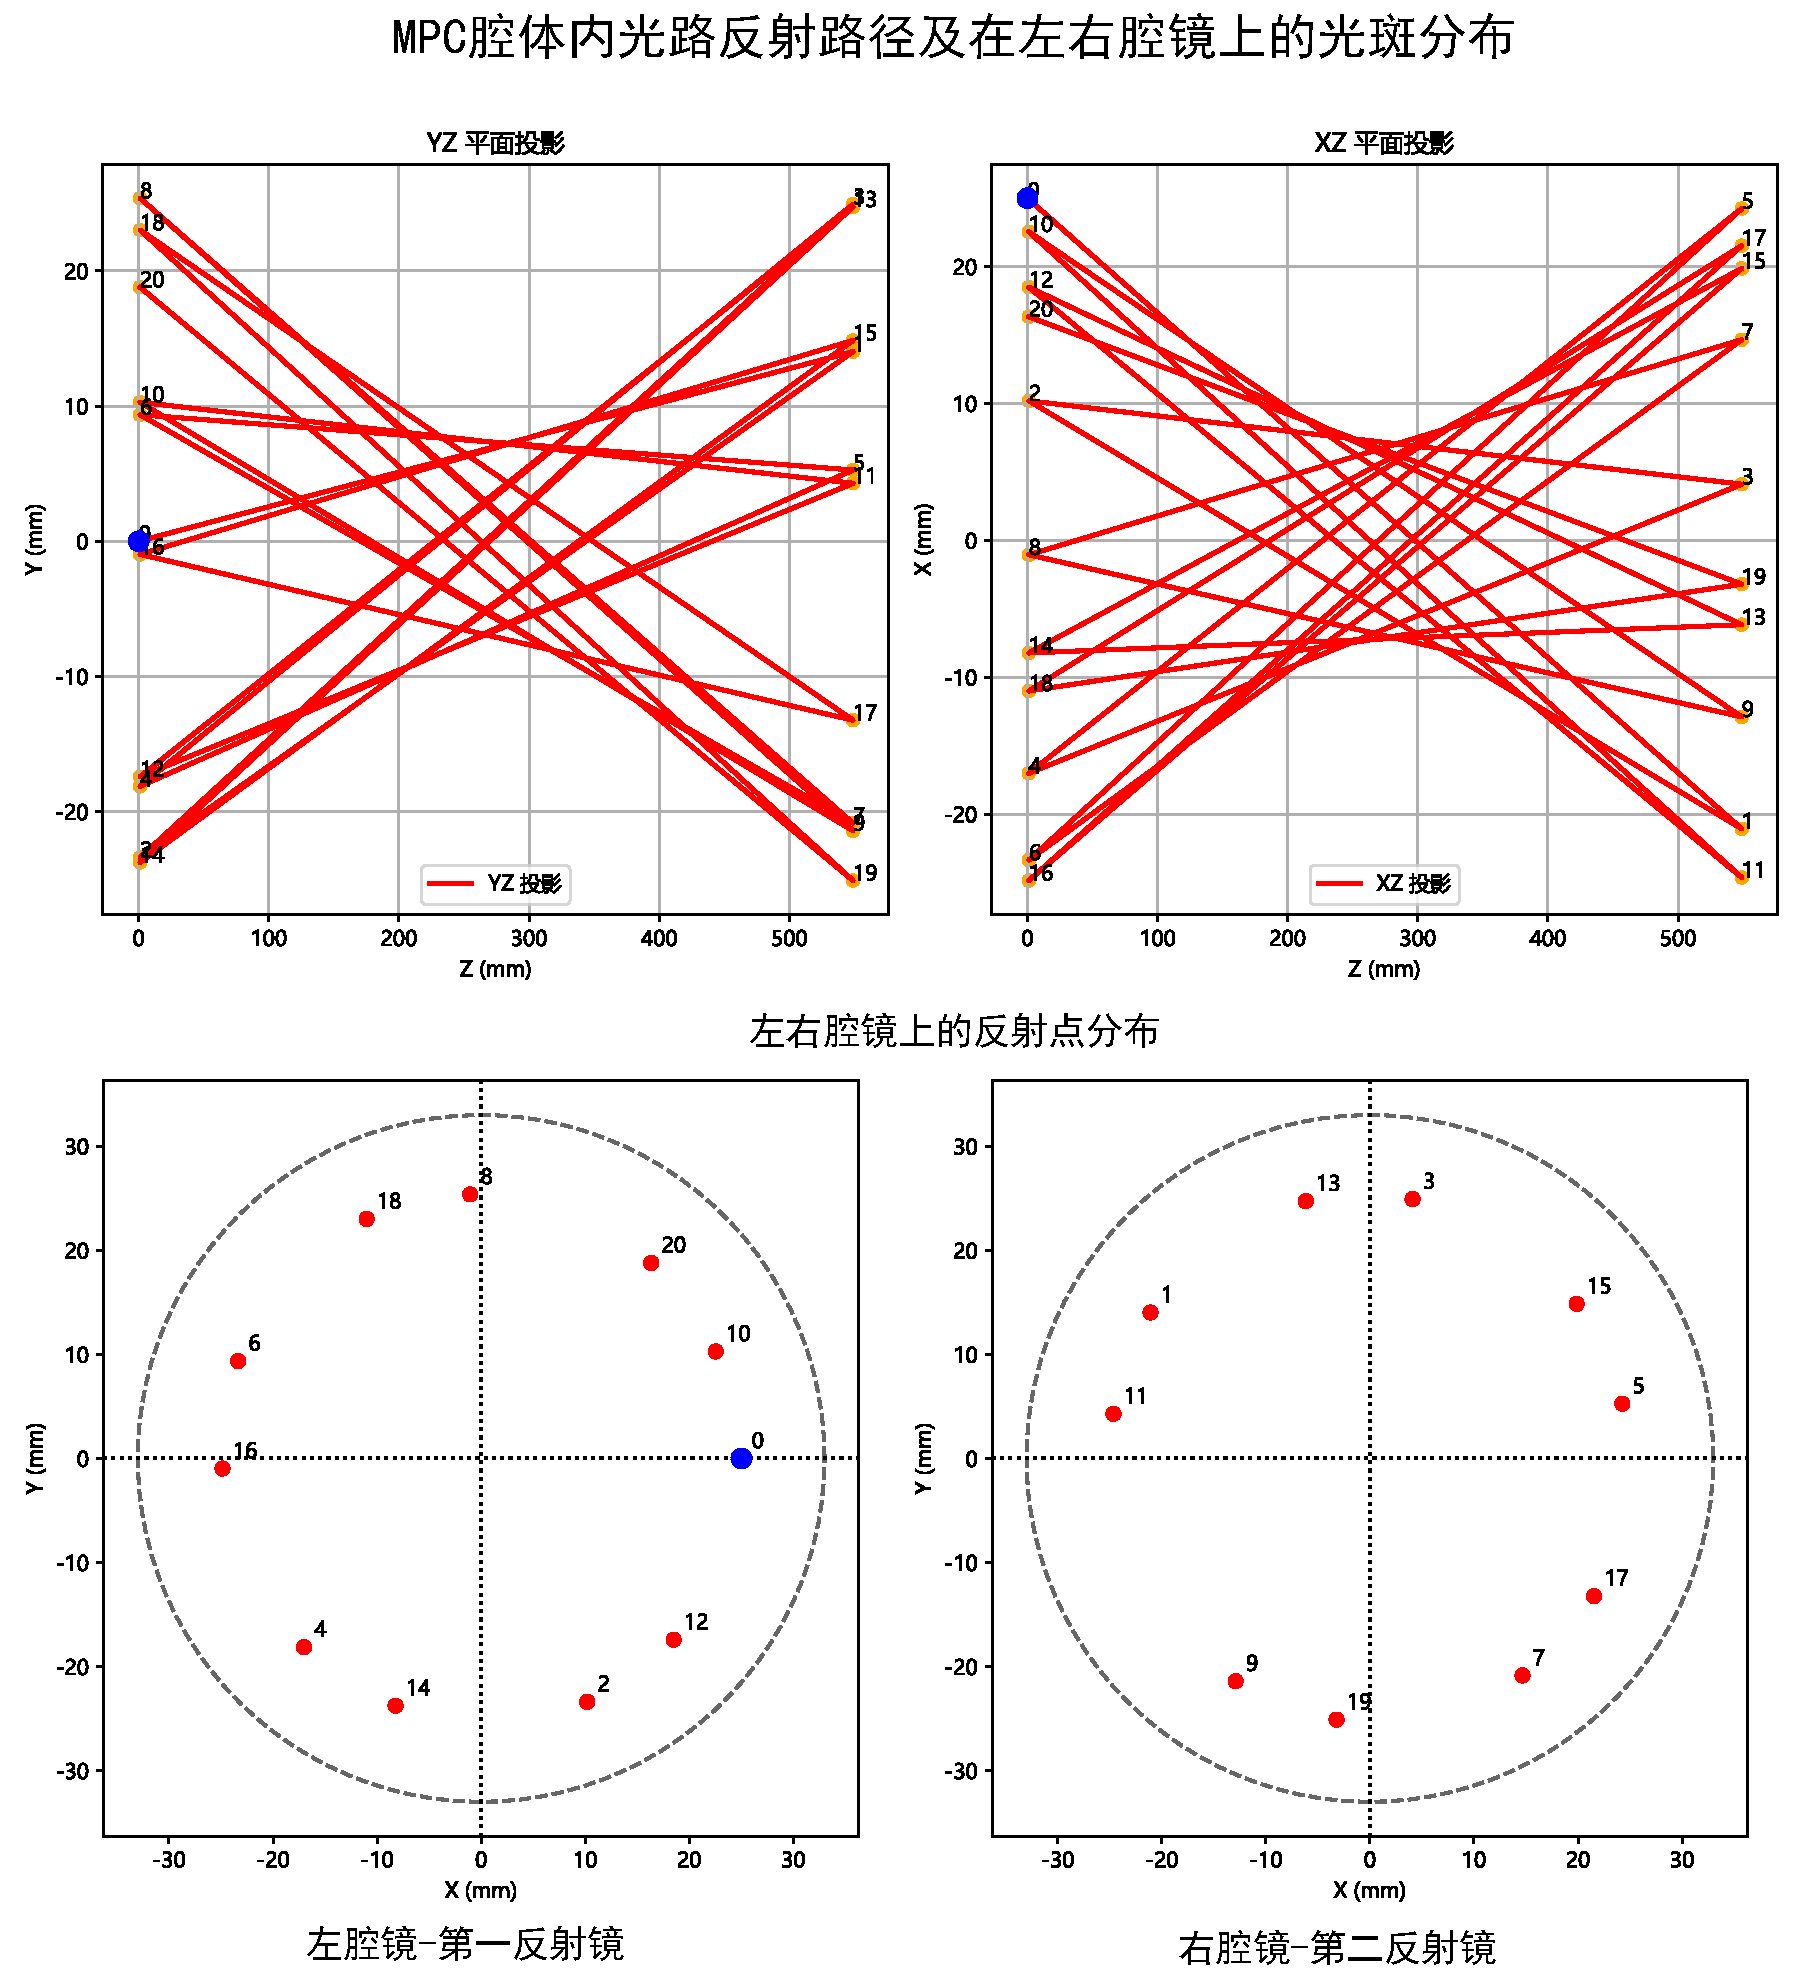
\includegraphics[width=\textwidth]{Fig/MPC-Figure_4.pdf}
        \caption{}
        \label{fig:mpc_geometry_a}
    \end{subfigure}
    \hfil
    \begin{subfigure}[b]{0.38\textwidth}
        \centering
        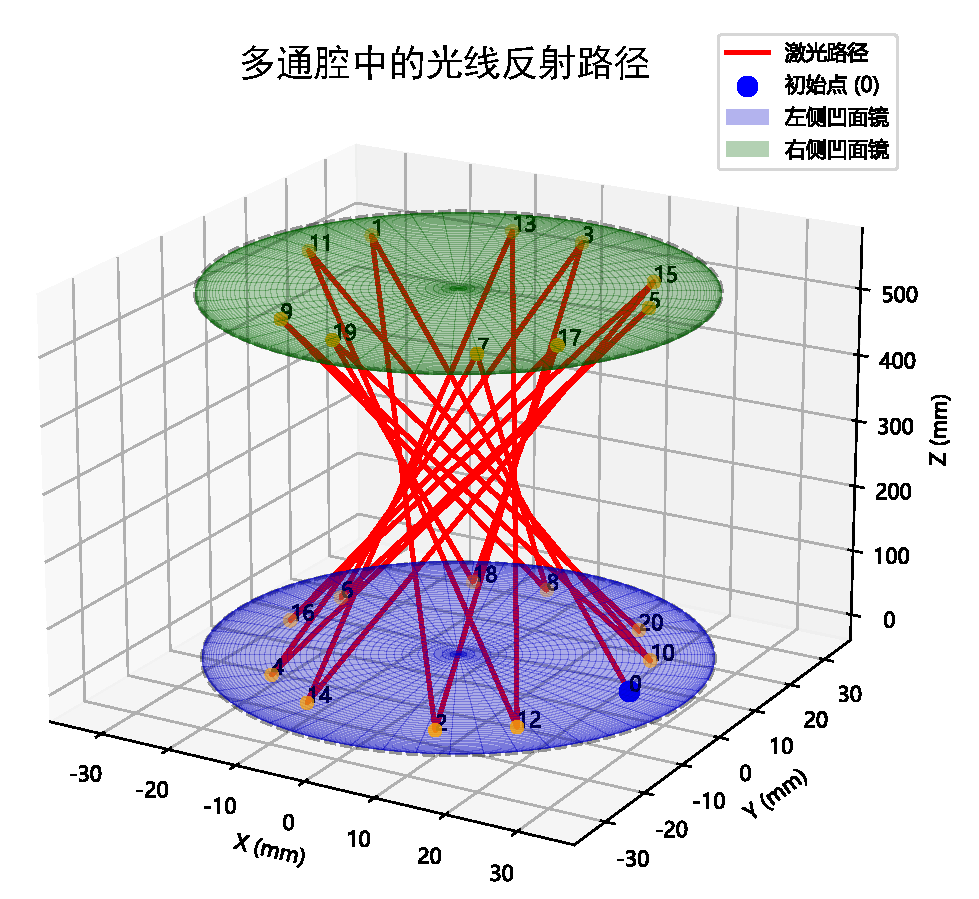
\includegraphics[width=\textwidth]{Fig/MPC-Figure_3.pdf}
        \caption{}
        \label{fig:mpc_geometry_b}
    \end{subfigure}

    \bicaption{Herriott 型多通腔的几何结构与传播路径仿真结果。(a)光束在 $YZ$ 和 $XZ$ 平面中的投影轨迹及左右腔镜上的反射点分布；(b)腔内三维光线反射路径示意图}
    {Geometric and ray-tracing simulation results of the Herriott-type multipass cavity. (a) Projected ray trajectories in the $YZ$ and $XZ$ planes and the reflection-spot distributions on the two cavity mirrors; (b) three-dimensional ray-reflection path inside the cavity}
    \label{fig:mpc_geometry}
\end{figure}

如图~\ref{fig:mpc_geometry}所示，图~\ref{fig:mpc_geometry}(\subref{fig:mpc_geometry_a}) 给出了光束在 $YZ$ 和 $XZ$ 平面内的投影轨迹以及左右腔镜上的反射点分布；图~\ref{fig:mpc_geometry}(\subref{fig:mpc_geometry_b}) 则进一步展示了腔内三维光线反射路径。结果表明，在当前参数下，光束能够在腔镜有效口径范围内形成稳定且分散的多次反射轨迹，为后续非线性光谱展宽提供了空间基础。



\subsubsection{MPC 时频域压缩结果}
在完成腔体几何设计后，本文进一步对脉冲在 MPC 中的时频域演化进行了仿真。结果表明，脉冲经过多次往返传播后可在非线性介质中积累显著的自相位调制，从而实现明显的光谱展宽；在进一步引入二阶色散补偿后，展宽后的脉冲可被压缩至数十飞秒量级。图~\ref{fig:mpc_compression}(\subref{fig:mpc_compression_a}) 给出了压缩前后的时域脉冲对比，图~\ref{fig:mpc_compression}(\subref{fig:mpc_compression_b}) 给出了对应的频域光谱展宽结果。


\begin{figure}[htbp]
    \centering
    \begin{subfigure}[b]{0.48\textwidth}
        \centering
        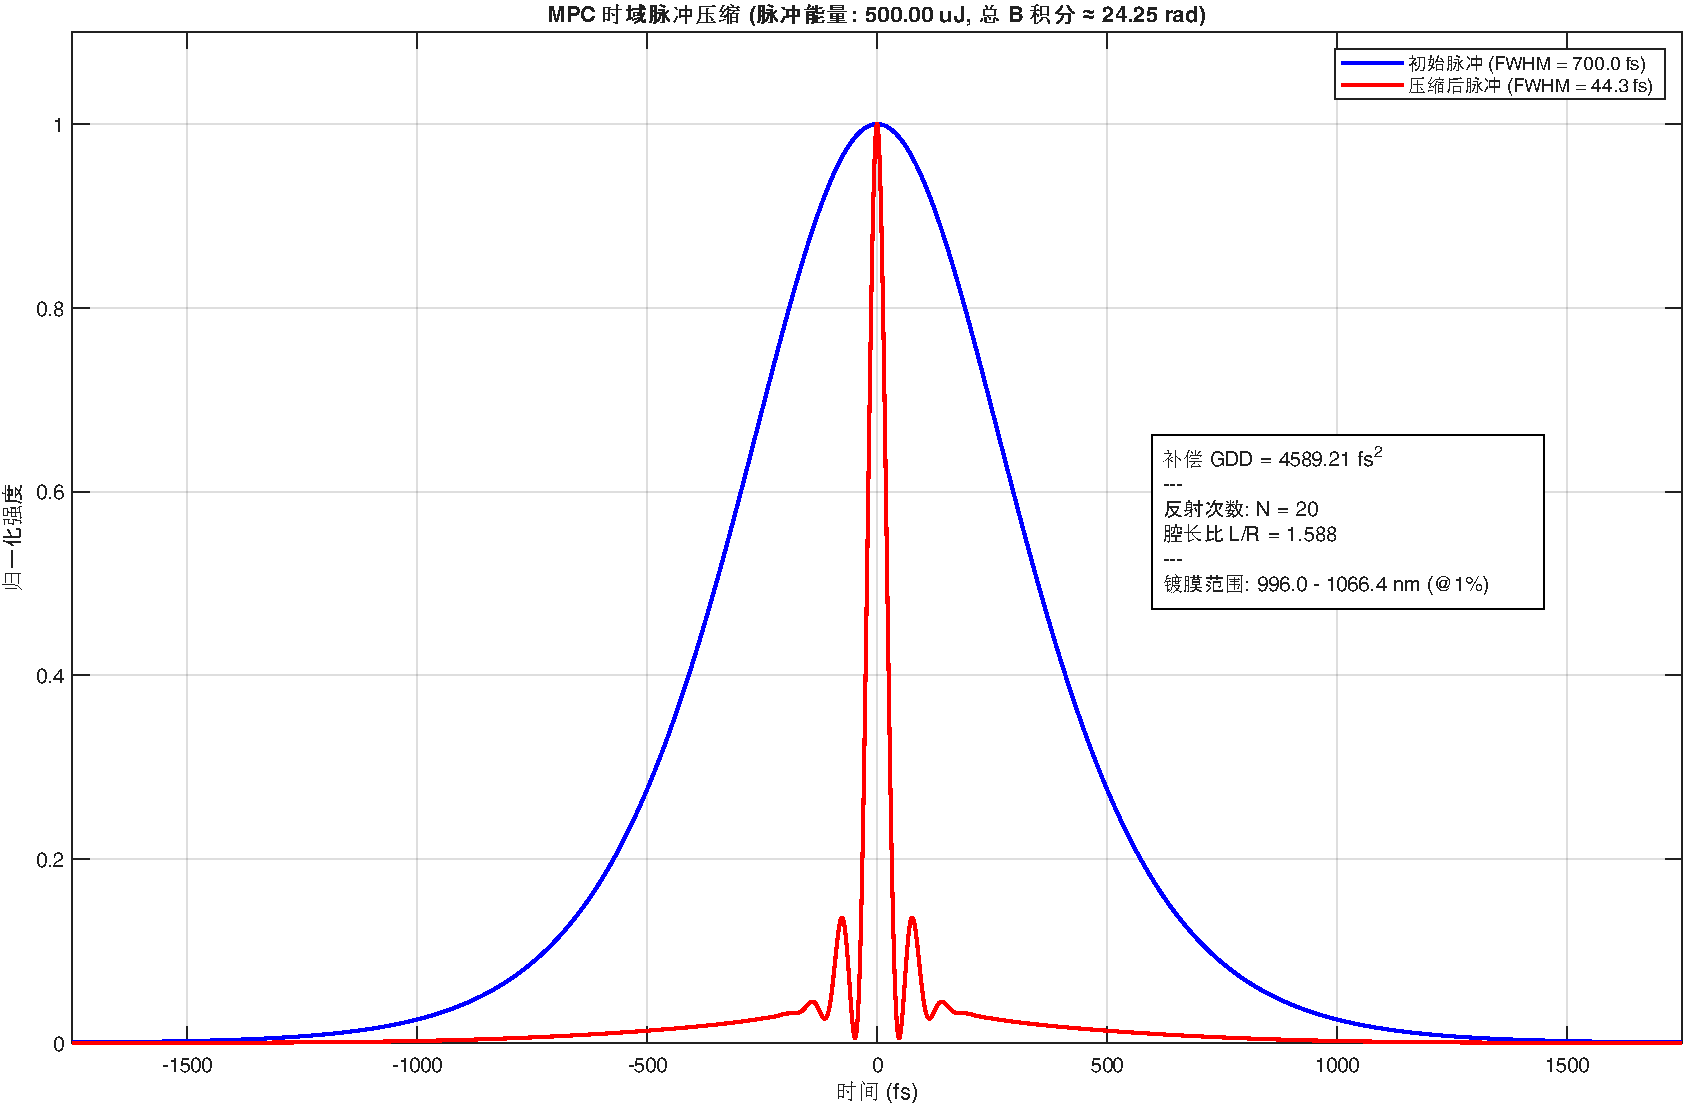
\includegraphics[width=\textwidth]{Fig/MPC-Figure_7.pdf}
        \caption{}
        \label{fig:mpc_compression_a}
    \end{subfigure}
    \hfil
    \begin{subfigure}[b]{0.48\textwidth}
        \centering
        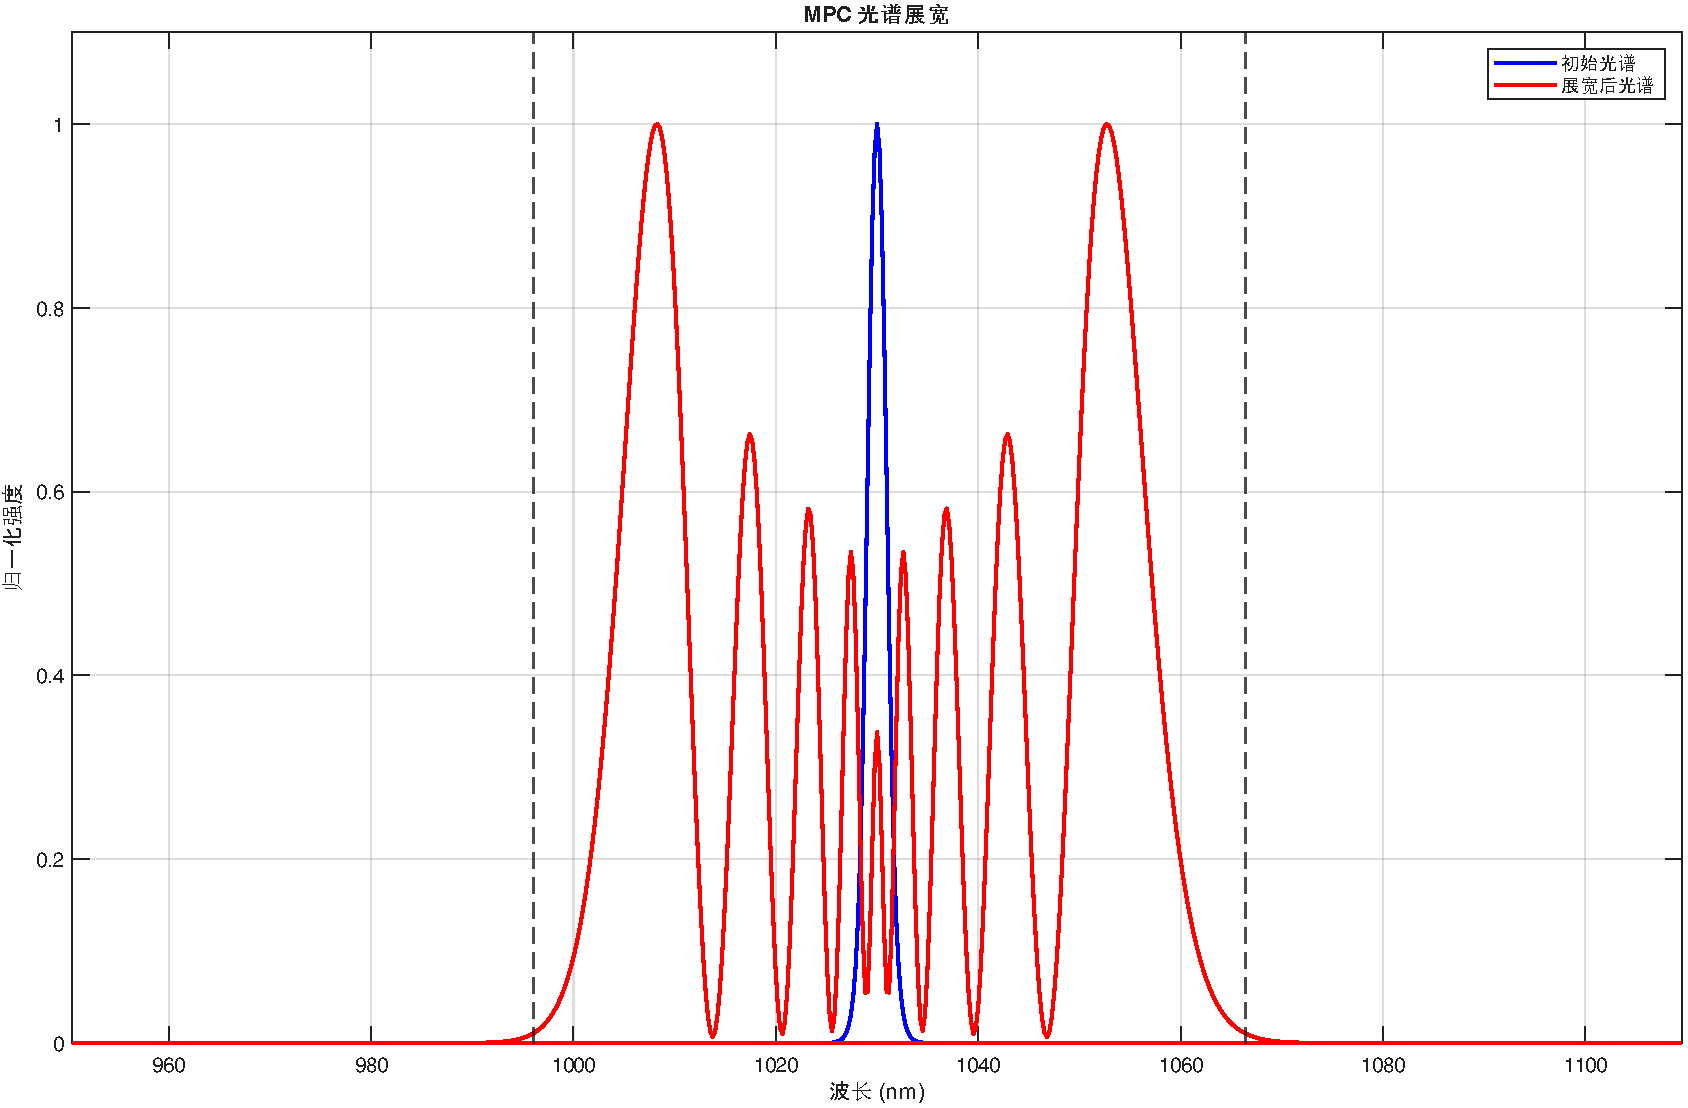
\includegraphics[width=\textwidth]{Fig/MPC-Figure_8.pdf}
        \caption{}
        \label{fig:mpc_compression_b}
    \end{subfigure}

    \bicaption{MPC 压缩过程的时频域仿真结果。(a)压缩前后时域脉冲对比；(b)压缩前后频域光谱对比}
    {Time- and frequency-domain simulation results of the MPC compression process. (a) Temporal profiles before and after compression; (b) spectra before and after compression}
    \label{fig:mpc_compression}
\end{figure}

在最终选取的腔体参数下，初始半高全宽约为 700 fs 的 1030 nm 脉冲在 MPC 中经多次往返传播并结合二阶色散补偿后，可进一步压缩至131.75fs。

完成上述多光子平台搭建与脉冲调控后，系统已具备开展时间分辨荧光寿命采集的基本条件；因此，下一章将进一步围绕 TCSPC 同步采集、数据重建与寿命拟合算法展开分析。